\documentclass[twoside]{book}

% Packages required by doxygen
\usepackage{fixltx2e}
\usepackage{calc}
\usepackage{doxygen}
\usepackage[export]{adjustbox} % also loads graphicx
\usepackage{graphicx}
\usepackage[utf8]{inputenc}
\usepackage{makeidx}
\usepackage{multicol}
\usepackage{multirow}
\PassOptionsToPackage{warn}{textcomp}
\usepackage{textcomp}
\usepackage[nointegrals]{wasysym}
\usepackage[table]{xcolor}

% Font selection
\usepackage[T1]{fontenc}
\usepackage[scaled=.90]{helvet}
\usepackage{courier}
\usepackage{amssymb}
\usepackage{sectsty}
\renewcommand{\familydefault}{\sfdefault}
\allsectionsfont{%
  \fontseries{bc}\selectfont%
  \color{darkgray}%
}
\renewcommand{\DoxyLabelFont}{%
  \fontseries{bc}\selectfont%
  \color{darkgray}%
}
\newcommand{\+}{\discretionary{\mbox{\scriptsize$\hookleftarrow$}}{}{}}

% Page & text layout
\usepackage{geometry}
\geometry{%
  a4paper,%
  top=2.5cm,%
  bottom=2.5cm,%
  left=2.5cm,%
  right=2.5cm%
}
\tolerance=750
\hfuzz=15pt
\hbadness=750
\setlength{\emergencystretch}{15pt}
\setlength{\parindent}{0cm}
\setlength{\parskip}{0.2cm}
\makeatletter
\renewcommand{\paragraph}{%
  \@startsection{paragraph}{4}{0ex}{-1.0ex}{1.0ex}{%
    \normalfont\normalsize\bfseries\SS@parafont%
  }%
}
\renewcommand{\subparagraph}{%
  \@startsection{subparagraph}{5}{0ex}{-1.0ex}{1.0ex}{%
    \normalfont\normalsize\bfseries\SS@subparafont%
  }%
}
\makeatother

% Headers & footers
\usepackage{fancyhdr}
\pagestyle{fancyplain}
\fancyhead[LE]{\fancyplain{}{\bfseries\thepage}}
\fancyhead[CE]{\fancyplain{}{}}
\fancyhead[RE]{\fancyplain{}{\bfseries\leftmark}}
\fancyhead[LO]{\fancyplain{}{\bfseries\rightmark}}
\fancyhead[CO]{\fancyplain{}{}}
\fancyhead[RO]{\fancyplain{}{\bfseries\thepage}}
\fancyfoot[LE]{\fancyplain{}{}}
\fancyfoot[CE]{\fancyplain{}{}}
\fancyfoot[RE]{\fancyplain{}{\bfseries\scriptsize Generated on Thu May 28 2015 15\+:01\+:53 for My Project by Doxygen }}
\fancyfoot[LO]{\fancyplain{}{\bfseries\scriptsize Generated on Thu May 28 2015 15\+:01\+:53 for My Project by Doxygen }}
\fancyfoot[CO]{\fancyplain{}{}}
\fancyfoot[RO]{\fancyplain{}{}}
\renewcommand{\footrulewidth}{0.4pt}
\renewcommand{\chaptermark}[1]{%
  \markboth{#1}{}%
}
\renewcommand{\sectionmark}[1]{%
  \markright{\thesection\ #1}%
}

% Indices & bibliography
\usepackage{natbib}
\usepackage[titles]{tocloft}
\setcounter{tocdepth}{3}
\setcounter{secnumdepth}{5}
\makeindex

% Hyperlinks (required, but should be loaded last)
\usepackage{ifpdf}
\ifpdf
  \usepackage[pdftex,pagebackref=true]{hyperref}
\else
  \usepackage[ps2pdf,pagebackref=true]{hyperref}
\fi
\hypersetup{%
  colorlinks=true,%
  linkcolor=blue,%
  citecolor=blue,%
  unicode%
}

% Custom commands
\newcommand{\clearemptydoublepage}{%
  \newpage{\pagestyle{empty}\cleardoublepage}%
}


%===== C O N T E N T S =====

\begin{document}

% Titlepage & ToC
\hypersetup{pageanchor=false,
             bookmarks=true,
             bookmarksnumbered=true,
             pdfencoding=unicode
            }
\pagenumbering{roman}
\begin{titlepage}
\vspace*{7cm}
\begin{center}%
{\Large My Project }\\
\vspace*{1cm}
{\large Generated by Doxygen 1.8.9.1}\\
\vspace*{0.5cm}
{\small Thu May 28 2015 15:01:53}\\
\end{center}
\end{titlepage}
\clearemptydoublepage
\tableofcontents
\clearemptydoublepage
\pagenumbering{arabic}
\hypersetup{pageanchor=true}

%--- Begin generated contents ---
\chapter{Hierarchical Index}
\section{Class Hierarchy}
This inheritance list is sorted roughly, but not completely, alphabetically\+:\begin{DoxyCompactList}
\item \contentsline{section}{Sim\+G\+D\+C.\+action\+Handler.\+Action\+Handler}{\pageref{class_sim_g_d_c_1_1action_handler_1_1_action_handler}}{}
\item object\begin{DoxyCompactList}
\item \contentsline{section}{Sim\+G\+D\+C.\+ui\+\_\+busstop.\+Ui\+\_\+\+Busstop}{\pageref{class_sim_g_d_c_1_1ui__busstop_1_1_ui___busstop}}{}
\item \contentsline{section}{Sim\+G\+D\+C.\+ui\+\_\+converter.\+Ui\+\_\+\+Converter}{\pageref{class_sim_g_d_c_1_1ui__converter_1_1_ui___converter}}{}
\item \contentsline{section}{Sim\+G\+D\+C.\+ui\+\_\+crossing.\+Ui\+\_\+\+Crossing}{\pageref{class_sim_g_d_c_1_1ui__crossing_1_1_ui___crossing}}{}
\item \contentsline{section}{Sim\+G\+D\+C.\+ui\+\_\+lane.\+Ui\+\_\+\+Lane}{\pageref{class_sim_g_d_c_1_1ui__lane_1_1_ui___lane}}{}
\item \contentsline{section}{Sim\+G\+D\+C.\+ui\+\_\+laneedge.\+Ui\+\_\+\+Lane\+Edge}{\pageref{class_sim_g_d_c_1_1ui__laneedge_1_1_ui___lane_edge}}{}
\item \contentsline{section}{Sim\+G\+D\+C.\+ui\+\_\+linkmanager.\+Ui\+\_\+\+Link\+Manager}{\pageref{class_sim_g_d_c_1_1ui__linkmanager_1_1_ui___link_manager}}{}
\item \contentsline{section}{Sim\+G\+D\+C.\+ui\+\_\+multinode.\+Ui\+\_\+\+Multi\+Node}{\pageref{class_sim_g_d_c_1_1ui__multinode_1_1_ui___multi_node}}{}
\item \contentsline{section}{Sim\+G\+D\+C.\+ui\+\_\+segment.\+Ui\+\_\+\+Segment}{\pageref{class_sim_g_d_c_1_1ui__segment_1_1_ui___segment}}{}
\item \contentsline{section}{Sim\+G\+D\+C.\+ui\+\_\+trainstop.\+Ui\+\_\+\+Train\+Stop}{\pageref{class_sim_g_d_c_1_1ui__trainstop_1_1_ui___train_stop}}{}
\end{DoxyCompactList}
\item Q\+Dialog\begin{DoxyCompactList}
\item \contentsline{section}{Sim\+G\+D\+C.\+busstop\+\_\+dialog.\+Busstop\+Dialog}{\pageref{class_sim_g_d_c_1_1busstop__dialog_1_1_busstop_dialog}}{}
\item \contentsline{section}{Sim\+G\+D\+C.\+converter\+\_\+dialog.\+Converter\+Dialog}{\pageref{class_sim_g_d_c_1_1converter__dialog_1_1_converter_dialog}}{}
\item \contentsline{section}{Sim\+G\+D\+C.\+crossing\+\_\+dialog.\+Crossing\+Dialog}{\pageref{class_sim_g_d_c_1_1crossing__dialog_1_1_crossing_dialog}}{}
\item \contentsline{section}{Sim\+G\+D\+C.\+lane\+\_\+dialog.\+Lane\+Dialog}{\pageref{class_sim_g_d_c_1_1lane__dialog_1_1_lane_dialog}}{}
\item \contentsline{section}{Sim\+G\+D\+C.\+laneedge\+\_\+dialog.\+Lane\+Edge\+Dialog}{\pageref{class_sim_g_d_c_1_1laneedge__dialog_1_1_lane_edge_dialog}}{}
\item \contentsline{section}{Sim\+G\+D\+C.\+linkmanager\+\_\+dialog.\+Link\+Manager\+Dialog}{\pageref{class_sim_g_d_c_1_1linkmanager__dialog_1_1_link_manager_dialog}}{}
\item \contentsline{section}{Sim\+G\+D\+C.\+multinode\+\_\+dialog.\+Multi\+Node\+Dialog}{\pageref{class_sim_g_d_c_1_1multinode__dialog_1_1_multi_node_dialog}}{}
\item \contentsline{section}{Sim\+G\+D\+C.\+segment\+\_\+dialog.\+Segment\+Dialog}{\pageref{class_sim_g_d_c_1_1segment__dialog_1_1_segment_dialog}}{}
\item \contentsline{section}{Sim\+G\+D\+C.\+trainstop\+\_\+dialog.\+Trainstop\+Dialog}{\pageref{class_sim_g_d_c_1_1trainstop__dialog_1_1_trainstop_dialog}}{}
\end{DoxyCompactList}
\item Q\+Object\begin{DoxyCompactList}
\item \contentsline{section}{Sim\+G\+D\+C.\+shapefile\+To\+Xml.\+Shapefile\+To\+Xml}{\pageref{class_sim_g_d_c_1_1shapefile_to_xml_1_1_shapefile_to_xml}}{}
\item \contentsline{section}{Sim\+G\+D\+C.\+xml\+To\+Shapefile.\+Xml\+To\+Shapefile}{\pageref{class_sim_g_d_c_1_1xml_to_shapefile_1_1_xml_to_shapefile}}{}
\end{DoxyCompactList}
\item \contentsline{section}{Sim\+G\+D\+C.\+shapefile\+I\+O.\+Shapefile\+Reader}{\pageref{class_sim_g_d_c_1_1shapefile_i_o_1_1_shapefile_reader}}{}
\item \contentsline{section}{Sim\+G\+D\+C.\+shapefile\+I\+O.\+Shapefile\+Writer}{\pageref{class_sim_g_d_c_1_1shapefile_i_o_1_1_shapefile_writer}}{}
\item \contentsline{section}{Sim\+G\+D\+C.\+simgdc.\+Sim\+G\+D\+C}{\pageref{class_sim_g_d_c_1_1simgdc_1_1_sim_g_d_c}}{}
\item Ui\+\_\+\+Busstop\begin{DoxyCompactList}
\item \contentsline{section}{Sim\+G\+D\+C.\+busstop\+\_\+dialog.\+Busstop\+Dialog}{\pageref{class_sim_g_d_c_1_1busstop__dialog_1_1_busstop_dialog}}{}
\end{DoxyCompactList}
\item Ui\+\_\+\+Converter\begin{DoxyCompactList}
\item \contentsline{section}{Sim\+G\+D\+C.\+converter\+\_\+dialog.\+Converter\+Dialog}{\pageref{class_sim_g_d_c_1_1converter__dialog_1_1_converter_dialog}}{}
\end{DoxyCompactList}
\item Ui\+\_\+\+Crossing\begin{DoxyCompactList}
\item \contentsline{section}{Sim\+G\+D\+C.\+crossing\+\_\+dialog.\+Crossing\+Dialog}{\pageref{class_sim_g_d_c_1_1crossing__dialog_1_1_crossing_dialog}}{}
\end{DoxyCompactList}
\item Ui\+\_\+\+Lane\begin{DoxyCompactList}
\item \contentsline{section}{Sim\+G\+D\+C.\+lane\+\_\+dialog.\+Lane\+Dialog}{\pageref{class_sim_g_d_c_1_1lane__dialog_1_1_lane_dialog}}{}
\end{DoxyCompactList}
\item Ui\+\_\+\+Lane\+Edge\begin{DoxyCompactList}
\item \contentsline{section}{Sim\+G\+D\+C.\+laneedge\+\_\+dialog.\+Lane\+Edge\+Dialog}{\pageref{class_sim_g_d_c_1_1laneedge__dialog_1_1_lane_edge_dialog}}{}
\end{DoxyCompactList}
\item Ui\+\_\+\+Link\+Manager\begin{DoxyCompactList}
\item \contentsline{section}{Sim\+G\+D\+C.\+linkmanager\+\_\+dialog.\+Link\+Manager\+Dialog}{\pageref{class_sim_g_d_c_1_1linkmanager__dialog_1_1_link_manager_dialog}}{}
\end{DoxyCompactList}
\item Ui\+\_\+\+Multi\+Node\begin{DoxyCompactList}
\item \contentsline{section}{Sim\+G\+D\+C.\+multinode\+\_\+dialog.\+Multi\+Node\+Dialog}{\pageref{class_sim_g_d_c_1_1multinode__dialog_1_1_multi_node_dialog}}{}
\end{DoxyCompactList}
\item Ui\+\_\+\+Segment\begin{DoxyCompactList}
\item \contentsline{section}{Sim\+G\+D\+C.\+segment\+\_\+dialog.\+Segment\+Dialog}{\pageref{class_sim_g_d_c_1_1segment__dialog_1_1_segment_dialog}}{}
\end{DoxyCompactList}
\item Ui\+\_\+\+Train\+Stop\begin{DoxyCompactList}
\item \contentsline{section}{Sim\+G\+D\+C.\+trainstop\+\_\+dialog.\+Trainstop\+Dialog}{\pageref{class_sim_g_d_c_1_1trainstop__dialog_1_1_trainstop_dialog}}{}
\end{DoxyCompactList}
\end{DoxyCompactList}

\chapter{Class Index}
\section{Class List}
Here are the classes, structs, unions and interfaces with brief descriptions\+:\begin{DoxyCompactList}
\item\contentsline{section}{\hyperlink{class_sim_g_d_c_1_1action_handler_1_1_action_handler}{Sim\+G\+D\+C.\+action\+Handler.\+Action\+Handler} }{\pageref{class_sim_g_d_c_1_1action_handler_1_1_action_handler}}{}
\item\contentsline{section}{\hyperlink{class_sim_g_d_c_1_1busstop__dialog_1_1_busstop_dialog}{Sim\+G\+D\+C.\+busstop\+\_\+dialog.\+Busstop\+Dialog} }{\pageref{class_sim_g_d_c_1_1busstop__dialog_1_1_busstop_dialog}}{}
\item\contentsline{section}{\hyperlink{class_sim_g_d_c_1_1converter__dialog_1_1_converter_dialog}{Sim\+G\+D\+C.\+converter\+\_\+dialog.\+Converter\+Dialog} }{\pageref{class_sim_g_d_c_1_1converter__dialog_1_1_converter_dialog}}{}
\item\contentsline{section}{\hyperlink{class_sim_g_d_c_1_1crossing__dialog_1_1_crossing_dialog}{Sim\+G\+D\+C.\+crossing\+\_\+dialog.\+Crossing\+Dialog} }{\pageref{class_sim_g_d_c_1_1crossing__dialog_1_1_crossing_dialog}}{}
\item\contentsline{section}{\hyperlink{class_sim_g_d_c_1_1lane__dialog_1_1_lane_dialog}{Sim\+G\+D\+C.\+lane\+\_\+dialog.\+Lane\+Dialog} }{\pageref{class_sim_g_d_c_1_1lane__dialog_1_1_lane_dialog}}{}
\item\contentsline{section}{\hyperlink{class_sim_g_d_c_1_1laneedge__dialog_1_1_lane_edge_dialog}{Sim\+G\+D\+C.\+laneedge\+\_\+dialog.\+Lane\+Edge\+Dialog} }{\pageref{class_sim_g_d_c_1_1laneedge__dialog_1_1_lane_edge_dialog}}{}
\item\contentsline{section}{\hyperlink{class_sim_g_d_c_1_1linkmanager__dialog_1_1_link_manager_dialog}{Sim\+G\+D\+C.\+linkmanager\+\_\+dialog.\+Link\+Manager\+Dialog} }{\pageref{class_sim_g_d_c_1_1linkmanager__dialog_1_1_link_manager_dialog}}{}
\item\contentsline{section}{\hyperlink{class_sim_g_d_c_1_1multinode__dialog_1_1_multi_node_dialog}{Sim\+G\+D\+C.\+multinode\+\_\+dialog.\+Multi\+Node\+Dialog} }{\pageref{class_sim_g_d_c_1_1multinode__dialog_1_1_multi_node_dialog}}{}
\item\contentsline{section}{\hyperlink{class_sim_g_d_c_1_1segment__dialog_1_1_segment_dialog}{Sim\+G\+D\+C.\+segment\+\_\+dialog.\+Segment\+Dialog} }{\pageref{class_sim_g_d_c_1_1segment__dialog_1_1_segment_dialog}}{}
\item\contentsline{section}{\hyperlink{class_sim_g_d_c_1_1shapefile_i_o_1_1_shapefile_reader}{Sim\+G\+D\+C.\+shapefile\+I\+O.\+Shapefile\+Reader} }{\pageref{class_sim_g_d_c_1_1shapefile_i_o_1_1_shapefile_reader}}{}
\item\contentsline{section}{\hyperlink{class_sim_g_d_c_1_1shapefile_to_xml_1_1_shapefile_to_xml}{Sim\+G\+D\+C.\+shapefile\+To\+Xml.\+Shapefile\+To\+Xml} }{\pageref{class_sim_g_d_c_1_1shapefile_to_xml_1_1_shapefile_to_xml}}{}
\item\contentsline{section}{\hyperlink{class_sim_g_d_c_1_1shapefile_i_o_1_1_shapefile_writer}{Sim\+G\+D\+C.\+shapefile\+I\+O.\+Shapefile\+Writer} }{\pageref{class_sim_g_d_c_1_1shapefile_i_o_1_1_shapefile_writer}}{}
\item\contentsline{section}{\hyperlink{class_sim_g_d_c_1_1simgdc_1_1_sim_g_d_c}{Sim\+G\+D\+C.\+simgdc.\+Sim\+G\+D\+C} }{\pageref{class_sim_g_d_c_1_1simgdc_1_1_sim_g_d_c}}{}
\item\contentsline{section}{\hyperlink{class_sim_g_d_c_1_1trainstop__dialog_1_1_trainstop_dialog}{Sim\+G\+D\+C.\+trainstop\+\_\+dialog.\+Trainstop\+Dialog} }{\pageref{class_sim_g_d_c_1_1trainstop__dialog_1_1_trainstop_dialog}}{}
\item\contentsline{section}{\hyperlink{class_sim_g_d_c_1_1ui__busstop_1_1_ui___busstop}{Sim\+G\+D\+C.\+ui\+\_\+busstop.\+Ui\+\_\+\+Busstop} }{\pageref{class_sim_g_d_c_1_1ui__busstop_1_1_ui___busstop}}{}
\item\contentsline{section}{\hyperlink{class_sim_g_d_c_1_1ui__converter_1_1_ui___converter}{Sim\+G\+D\+C.\+ui\+\_\+converter.\+Ui\+\_\+\+Converter} }{\pageref{class_sim_g_d_c_1_1ui__converter_1_1_ui___converter}}{}
\item\contentsline{section}{\hyperlink{class_sim_g_d_c_1_1ui__crossing_1_1_ui___crossing}{Sim\+G\+D\+C.\+ui\+\_\+crossing.\+Ui\+\_\+\+Crossing} }{\pageref{class_sim_g_d_c_1_1ui__crossing_1_1_ui___crossing}}{}
\item\contentsline{section}{\hyperlink{class_sim_g_d_c_1_1ui__lane_1_1_ui___lane}{Sim\+G\+D\+C.\+ui\+\_\+lane.\+Ui\+\_\+\+Lane} }{\pageref{class_sim_g_d_c_1_1ui__lane_1_1_ui___lane}}{}
\item\contentsline{section}{\hyperlink{class_sim_g_d_c_1_1ui__laneedge_1_1_ui___lane_edge}{Sim\+G\+D\+C.\+ui\+\_\+laneedge.\+Ui\+\_\+\+Lane\+Edge} }{\pageref{class_sim_g_d_c_1_1ui__laneedge_1_1_ui___lane_edge}}{}
\item\contentsline{section}{\hyperlink{class_sim_g_d_c_1_1ui__linkmanager_1_1_ui___link_manager}{Sim\+G\+D\+C.\+ui\+\_\+linkmanager.\+Ui\+\_\+\+Link\+Manager} }{\pageref{class_sim_g_d_c_1_1ui__linkmanager_1_1_ui___link_manager}}{}
\item\contentsline{section}{\hyperlink{class_sim_g_d_c_1_1ui__multinode_1_1_ui___multi_node}{Sim\+G\+D\+C.\+ui\+\_\+multinode.\+Ui\+\_\+\+Multi\+Node} }{\pageref{class_sim_g_d_c_1_1ui__multinode_1_1_ui___multi_node}}{}
\item\contentsline{section}{\hyperlink{class_sim_g_d_c_1_1ui__segment_1_1_ui___segment}{Sim\+G\+D\+C.\+ui\+\_\+segment.\+Ui\+\_\+\+Segment} }{\pageref{class_sim_g_d_c_1_1ui__segment_1_1_ui___segment}}{}
\item\contentsline{section}{\hyperlink{class_sim_g_d_c_1_1ui__trainstop_1_1_ui___train_stop}{Sim\+G\+D\+C.\+ui\+\_\+trainstop.\+Ui\+\_\+\+Train\+Stop} }{\pageref{class_sim_g_d_c_1_1ui__trainstop_1_1_ui___train_stop}}{}
\item\contentsline{section}{\hyperlink{class_sim_g_d_c_1_1xml_to_shapefile_1_1_xml_to_shapefile}{Sim\+G\+D\+C.\+xml\+To\+Shapefile.\+Xml\+To\+Shapefile} }{\pageref{class_sim_g_d_c_1_1xml_to_shapefile_1_1_xml_to_shapefile}}{}
\end{DoxyCompactList}

\chapter{Class Documentation}
\hypertarget{class_sim_g_d_c_1_1action_handler_1_1_action_handler}{}\section{Sim\+G\+D\+C.\+action\+Handler.\+Action\+Handler Class Reference}
\label{class_sim_g_d_c_1_1action_handler_1_1_action_handler}\index{Sim\+G\+D\+C.\+action\+Handler.\+Action\+Handler@{Sim\+G\+D\+C.\+action\+Handler.\+Action\+Handler}}
\subsection*{Public Member Functions}
\begin{DoxyCompactItemize}
\item 
\hypertarget{class_sim_g_d_c_1_1action_handler_1_1_action_handler_a7ce2b4e844e5130b34fc2be223cd1c4e}{}def {\bfseries \+\_\+\+\_\+init\+\_\+\+\_\+} (self, sh\+\_\+dir, canvas)\label{class_sim_g_d_c_1_1action_handler_1_1_action_handler_a7ce2b4e844e5130b34fc2be223cd1c4e}

\item 
\hypertarget{class_sim_g_d_c_1_1action_handler_1_1_action_handler_a00eaa01ee706b7bc6c51465847028ccd}{}def {\bfseries get\+Layer} (self, type\+Id)\label{class_sim_g_d_c_1_1action_handler_1_1_action_handler_a00eaa01ee706b7bc6c51465847028ccd}

\item 
def \hyperlink{class_sim_g_d_c_1_1action_handler_1_1_action_handler_af21ca70fa2e6a5358b9fcc8c8d3bc815}{add\+Multi\+Node} (self, point, node\+Data)
\item 
\hypertarget{class_sim_g_d_c_1_1action_handler_1_1_action_handler_abeaa8a461846ae07594a4cd69f7f85f1}{}def {\bfseries update\+Multi\+Node} (self, feature, node\+Data)\label{class_sim_g_d_c_1_1action_handler_1_1_action_handler_abeaa8a461846ae07594a4cd69f7f85f1}

\item 
\hypertarget{class_sim_g_d_c_1_1action_handler_1_1_action_handler_aeaed765d3f77de33bc6e760a7ae243af}{}def {\bfseries get\+Multi\+Node} (self, feature)\label{class_sim_g_d_c_1_1action_handler_1_1_action_handler_aeaed765d3f77de33bc6e760a7ae243af}

\item 
\hypertarget{class_sim_g_d_c_1_1action_handler_1_1_action_handler_a7846493d7f83224b40b3e8ac3ab26130}{}def {\bfseries get\+Link\+List} (self)\label{class_sim_g_d_c_1_1action_handler_1_1_action_handler_a7846493d7f83224b40b3e8ac3ab26130}

\item 
\hypertarget{class_sim_g_d_c_1_1action_handler_1_1_action_handler_ab48fa6a7f5bd67bcc258e44de0100ea5}{}def {\bfseries get\+Link\+List\+Detail} (self)\label{class_sim_g_d_c_1_1action_handler_1_1_action_handler_ab48fa6a7f5bd67bcc258e44de0100ea5}

\item 
\hypertarget{class_sim_g_d_c_1_1action_handler_1_1_action_handler_a9f5f150432351c24da2cdff6d8a877fb}{}def {\bfseries manage\+Link} (self, data)\label{class_sim_g_d_c_1_1action_handler_1_1_action_handler_a9f5f150432351c24da2cdff6d8a877fb}

\item 
def \hyperlink{class_sim_g_d_c_1_1action_handler_1_1_action_handler_a34e5dac56a9b8e37259041300e29469b}{add\+Segment} (self, point, data)
\item 
\hypertarget{class_sim_g_d_c_1_1action_handler_1_1_action_handler_a1d13b62e69eb09d281cbff8ff21e8816}{}def {\bfseries update\+Segment} (self, feature, data)\label{class_sim_g_d_c_1_1action_handler_1_1_action_handler_a1d13b62e69eb09d281cbff8ff21e8816}

\item 
\hypertarget{class_sim_g_d_c_1_1action_handler_1_1_action_handler_a0d328cac2adbcb37bde7b3ad6852e5d7}{}def {\bfseries get\+Segment} (self, feature)\label{class_sim_g_d_c_1_1action_handler_1_1_action_handler_a0d328cac2adbcb37bde7b3ad6852e5d7}

\item 
def \hyperlink{class_sim_g_d_c_1_1action_handler_1_1_action_handler_a5ca5aa78dcf765b9baf08a9f52672cc8}{add\+Crossing} (self, point, data)
\item 
\hypertarget{class_sim_g_d_c_1_1action_handler_1_1_action_handler_ae336445f7656cf4996e438c15cc3f354}{}def {\bfseries update\+Crossing} (self, feature, data)\label{class_sim_g_d_c_1_1action_handler_1_1_action_handler_ae336445f7656cf4996e438c15cc3f354}

\item 
\hypertarget{class_sim_g_d_c_1_1action_handler_1_1_action_handler_af868c73ea5b8412e6d700f9458477421}{}def {\bfseries get\+Crossing} (self, feature)\label{class_sim_g_d_c_1_1action_handler_1_1_action_handler_af868c73ea5b8412e6d700f9458477421}

\item 
def \hyperlink{class_sim_g_d_c_1_1action_handler_1_1_action_handler_a58203132da1e16c69647ea77a6eff342}{add\+Busstop} (self, point, data)
\item 
\hypertarget{class_sim_g_d_c_1_1action_handler_1_1_action_handler_a14a4f588524a61e443ed83d4a21ba425}{}def {\bfseries update\+Busstop} (self, feature, data)\label{class_sim_g_d_c_1_1action_handler_1_1_action_handler_a14a4f588524a61e443ed83d4a21ba425}

\item 
\hypertarget{class_sim_g_d_c_1_1action_handler_1_1_action_handler_af459cf3a87d3e97f83cdf15b538c381e}{}def {\bfseries get\+Busstop} (self, feature)\label{class_sim_g_d_c_1_1action_handler_1_1_action_handler_af459cf3a87d3e97f83cdf15b538c381e}

\item 
def \hyperlink{class_sim_g_d_c_1_1action_handler_1_1_action_handler_adfb8695cde259fc1634731c5f3fb7dd7}{add\+Trainstop} (self, point, data)
\item 
\hypertarget{class_sim_g_d_c_1_1action_handler_1_1_action_handler_a8b32e0ea018885b2107ffc4bfc707f13}{}def {\bfseries update\+Trainstop} (self, feature, data)\label{class_sim_g_d_c_1_1action_handler_1_1_action_handler_a8b32e0ea018885b2107ffc4bfc707f13}

\item 
\hypertarget{class_sim_g_d_c_1_1action_handler_1_1_action_handler_a8b4f5ac74bbeebfc4455a83cbfc4ae04}{}def {\bfseries get\+Trainstop} (self, feature)\label{class_sim_g_d_c_1_1action_handler_1_1_action_handler_a8b4f5ac74bbeebfc4455a83cbfc4ae04}

\item 
def \hyperlink{class_sim_g_d_c_1_1action_handler_1_1_action_handler_a5506d93ffa4d7aacfb1d2a339bf46acc}{add\+Lane} (self, point, data)
\item 
\hypertarget{class_sim_g_d_c_1_1action_handler_1_1_action_handler_a625096918b65e418a0b48f004bc76d9c}{}def {\bfseries update\+Lane} (self, feature, data)\label{class_sim_g_d_c_1_1action_handler_1_1_action_handler_a625096918b65e418a0b48f004bc76d9c}

\item 
\hypertarget{class_sim_g_d_c_1_1action_handler_1_1_action_handler_ad0057f117c1d077d2b1122f2b3a04168}{}def {\bfseries get\+Lane} (self, feature)\label{class_sim_g_d_c_1_1action_handler_1_1_action_handler_ad0057f117c1d077d2b1122f2b3a04168}

\item 
def \hyperlink{class_sim_g_d_c_1_1action_handler_1_1_action_handler_af08dcd34bf60677cdbaa4ac95f66e060}{add\+Lane\+Edge} (self, point, data)
\item 
\hypertarget{class_sim_g_d_c_1_1action_handler_1_1_action_handler_abd0c6c8b9fd34bc3708cfc17b5da23b1}{}def {\bfseries update\+Lane\+Edge} (self, feature, data)\label{class_sim_g_d_c_1_1action_handler_1_1_action_handler_abd0c6c8b9fd34bc3708cfc17b5da23b1}

\item 
\hypertarget{class_sim_g_d_c_1_1action_handler_1_1_action_handler_a6f26f54ffd6bfd20dbe005b76e66b3bd}{}def {\bfseries get\+Lane\+Edge} (self, feature)\label{class_sim_g_d_c_1_1action_handler_1_1_action_handler_a6f26f54ffd6bfd20dbe005b76e66b3bd}

\item 
\hypertarget{class_sim_g_d_c_1_1action_handler_1_1_action_handler_ae9a50ea441a506b5b7f1ed9b00da5683}{}def {\bfseries generate\+Lane\+By\+Number} (self, feature, n\+Lane, iwidth)\label{class_sim_g_d_c_1_1action_handler_1_1_action_handler_ae9a50ea441a506b5b7f1ed9b00da5683}

\item 
\hypertarget{class_sim_g_d_c_1_1action_handler_1_1_action_handler_acf17c7f2d1efab99b74f1104ec9bce96}{}def {\bfseries delete} (self, features)\label{class_sim_g_d_c_1_1action_handler_1_1_action_handler_acf17c7f2d1efab99b74f1104ec9bce96}

\item 
\hypertarget{class_sim_g_d_c_1_1action_handler_1_1_action_handler_a330249fb98d726327176f9afbfea3cb2}{}def {\bfseries delete\+Mul\+Node} (self, features)\label{class_sim_g_d_c_1_1action_handler_1_1_action_handler_a330249fb98d726327176f9afbfea3cb2}

\item 
\hypertarget{class_sim_g_d_c_1_1action_handler_1_1_action_handler_a4107cfaa0e0add3cecb24091cc470f97}{}def {\bfseries delete\+Bus\+Stop} (self, features)\label{class_sim_g_d_c_1_1action_handler_1_1_action_handler_a4107cfaa0e0add3cecb24091cc470f97}

\item 
\hypertarget{class_sim_g_d_c_1_1action_handler_1_1_action_handler_a1aef5ed34052ec54595df16874c64aa6}{}def {\bfseries delete\+Train\+Stop} (self, features)\label{class_sim_g_d_c_1_1action_handler_1_1_action_handler_a1aef5ed34052ec54595df16874c64aa6}

\item 
\hypertarget{class_sim_g_d_c_1_1action_handler_1_1_action_handler_af0c496565e3ef4fad5cab92b282079df}{}def {\bfseries delete\+Link} (self, features)\label{class_sim_g_d_c_1_1action_handler_1_1_action_handler_af0c496565e3ef4fad5cab92b282079df}

\item 
\hypertarget{class_sim_g_d_c_1_1action_handler_1_1_action_handler_aede14490d4d88bb7786199724fb10824}{}def {\bfseries delete\+Lane} (self, features)\label{class_sim_g_d_c_1_1action_handler_1_1_action_handler_aede14490d4d88bb7786199724fb10824}

\item 
\hypertarget{class_sim_g_d_c_1_1action_handler_1_1_action_handler_a9fbf1c291eaa48083e9de043d9b0b7ba}{}def {\bfseries delete\+Segment\+Components} (self, features)\label{class_sim_g_d_c_1_1action_handler_1_1_action_handler_a9fbf1c291eaa48083e9de043d9b0b7ba}

\item 
\hypertarget{class_sim_g_d_c_1_1action_handler_1_1_action_handler_a8d6dba3acc482964f4606d097a59a898}{}def {\bfseries delete\+Segment} (self, features)\label{class_sim_g_d_c_1_1action_handler_1_1_action_handler_a8d6dba3acc482964f4606d097a59a898}

\item 
\hypertarget{class_sim_g_d_c_1_1action_handler_1_1_action_handler_a2cff92ff0ae46393d7cd14660eb46342}{}def {\bfseries save} (self)\label{class_sim_g_d_c_1_1action_handler_1_1_action_handler_a2cff92ff0ae46393d7cd14660eb46342}

\end{DoxyCompactItemize}
\subsection*{Public Attributes}
\begin{DoxyCompactItemize}
\item 
\hypertarget{class_sim_g_d_c_1_1action_handler_1_1_action_handler_a743d8197483d597732d4d15c902f500d}{}{\bfseries sh\+\_\+dir}\label{class_sim_g_d_c_1_1action_handler_1_1_action_handler_a743d8197483d597732d4d15c902f500d}

\item 
\hypertarget{class_sim_g_d_c_1_1action_handler_1_1_action_handler_a093c807c0c683e59db16d3c7efc00223}{}{\bfseries data\+\_\+path}\label{class_sim_g_d_c_1_1action_handler_1_1_action_handler_a093c807c0c683e59db16d3c7efc00223}

\item 
\hypertarget{class_sim_g_d_c_1_1action_handler_1_1_action_handler_a24ac4ccceb1e511d26b7a46616503e76}{}{\bfseries document}\label{class_sim_g_d_c_1_1action_handler_1_1_action_handler_a24ac4ccceb1e511d26b7a46616503e76}

\item 
\hypertarget{class_sim_g_d_c_1_1action_handler_1_1_action_handler_a9484ed1ebc15bf2a183b0418219b5427}{}{\bfseries layers}\label{class_sim_g_d_c_1_1action_handler_1_1_action_handler_a9484ed1ebc15bf2a183b0418219b5427}

\item 
\hypertarget{class_sim_g_d_c_1_1action_handler_1_1_action_handler_a19ebd9b12b06a346204ee6e43ee09116}{}{\bfseries active\+\_\+layer}\label{class_sim_g_d_c_1_1action_handler_1_1_action_handler_a19ebd9b12b06a346204ee6e43ee09116}

\item 
\hypertarget{class_sim_g_d_c_1_1action_handler_1_1_action_handler_af7877e7cf1f84428808a020297507123}{}{\bfseries active\+\_\+layer\+\_\+id}\label{class_sim_g_d_c_1_1action_handler_1_1_action_handler_af7877e7cf1f84428808a020297507123}

\item 
\hypertarget{class_sim_g_d_c_1_1action_handler_1_1_action_handler_a7a2b7e45a23ddb72f065d07e71017157}{}{\bfseries prefix}\label{class_sim_g_d_c_1_1action_handler_1_1_action_handler_a7a2b7e45a23ddb72f065d07e71017157}

\end{DoxyCompactItemize}


\subsection{Member Function Documentation}
\hypertarget{class_sim_g_d_c_1_1action_handler_1_1_action_handler_a58203132da1e16c69647ea77a6eff342}{}\index{Sim\+G\+D\+C\+::action\+Handler\+::\+Action\+Handler@{Sim\+G\+D\+C\+::action\+Handler\+::\+Action\+Handler}!add\+Busstop@{add\+Busstop}}
\index{add\+Busstop@{add\+Busstop}!Sim\+G\+D\+C\+::action\+Handler\+::\+Action\+Handler@{Sim\+G\+D\+C\+::action\+Handler\+::\+Action\+Handler}}
\subsubsection[{add\+Busstop}]{\setlength{\rightskip}{0pt plus 5cm}def Sim\+G\+D\+C.\+action\+Handler.\+Action\+Handler.\+add\+Busstop (
\begin{DoxyParamCaption}
\item[{}]{self, }
\item[{}]{point, }
\item[{}]{data}
\end{DoxyParamCaption}
)}\label{class_sim_g_d_c_1_1action_handler_1_1_action_handler_a58203132da1e16c69647ea77a6eff342}
\begin{DoxyVerb}ADD FEATURE TO LAYER\end{DoxyVerb}
 \hypertarget{class_sim_g_d_c_1_1action_handler_1_1_action_handler_a5ca5aa78dcf765b9baf08a9f52672cc8}{}\index{Sim\+G\+D\+C\+::action\+Handler\+::\+Action\+Handler@{Sim\+G\+D\+C\+::action\+Handler\+::\+Action\+Handler}!add\+Crossing@{add\+Crossing}}
\index{add\+Crossing@{add\+Crossing}!Sim\+G\+D\+C\+::action\+Handler\+::\+Action\+Handler@{Sim\+G\+D\+C\+::action\+Handler\+::\+Action\+Handler}}
\subsubsection[{add\+Crossing}]{\setlength{\rightskip}{0pt plus 5cm}def Sim\+G\+D\+C.\+action\+Handler.\+Action\+Handler.\+add\+Crossing (
\begin{DoxyParamCaption}
\item[{}]{self, }
\item[{}]{point, }
\item[{}]{data}
\end{DoxyParamCaption}
)}\label{class_sim_g_d_c_1_1action_handler_1_1_action_handler_a5ca5aa78dcf765b9baf08a9f52672cc8}
\begin{DoxyVerb}ADD FEATURE TO LAYER\end{DoxyVerb}
 \hypertarget{class_sim_g_d_c_1_1action_handler_1_1_action_handler_a5506d93ffa4d7aacfb1d2a339bf46acc}{}\index{Sim\+G\+D\+C\+::action\+Handler\+::\+Action\+Handler@{Sim\+G\+D\+C\+::action\+Handler\+::\+Action\+Handler}!add\+Lane@{add\+Lane}}
\index{add\+Lane@{add\+Lane}!Sim\+G\+D\+C\+::action\+Handler\+::\+Action\+Handler@{Sim\+G\+D\+C\+::action\+Handler\+::\+Action\+Handler}}
\subsubsection[{add\+Lane}]{\setlength{\rightskip}{0pt plus 5cm}def Sim\+G\+D\+C.\+action\+Handler.\+Action\+Handler.\+add\+Lane (
\begin{DoxyParamCaption}
\item[{}]{self, }
\item[{}]{point, }
\item[{}]{data}
\end{DoxyParamCaption}
)}\label{class_sim_g_d_c_1_1action_handler_1_1_action_handler_a5506d93ffa4d7aacfb1d2a339bf46acc}
\begin{DoxyVerb}ADD FEATURE TO LAYER\end{DoxyVerb}
 \hypertarget{class_sim_g_d_c_1_1action_handler_1_1_action_handler_af08dcd34bf60677cdbaa4ac95f66e060}{}\index{Sim\+G\+D\+C\+::action\+Handler\+::\+Action\+Handler@{Sim\+G\+D\+C\+::action\+Handler\+::\+Action\+Handler}!add\+Lane\+Edge@{add\+Lane\+Edge}}
\index{add\+Lane\+Edge@{add\+Lane\+Edge}!Sim\+G\+D\+C\+::action\+Handler\+::\+Action\+Handler@{Sim\+G\+D\+C\+::action\+Handler\+::\+Action\+Handler}}
\subsubsection[{add\+Lane\+Edge}]{\setlength{\rightskip}{0pt plus 5cm}def Sim\+G\+D\+C.\+action\+Handler.\+Action\+Handler.\+add\+Lane\+Edge (
\begin{DoxyParamCaption}
\item[{}]{self, }
\item[{}]{point, }
\item[{}]{data}
\end{DoxyParamCaption}
)}\label{class_sim_g_d_c_1_1action_handler_1_1_action_handler_af08dcd34bf60677cdbaa4ac95f66e060}
\begin{DoxyVerb}ADD FEATURE TO LAYER\end{DoxyVerb}
 \hypertarget{class_sim_g_d_c_1_1action_handler_1_1_action_handler_af21ca70fa2e6a5358b9fcc8c8d3bc815}{}\index{Sim\+G\+D\+C\+::action\+Handler\+::\+Action\+Handler@{Sim\+G\+D\+C\+::action\+Handler\+::\+Action\+Handler}!add\+Multi\+Node@{add\+Multi\+Node}}
\index{add\+Multi\+Node@{add\+Multi\+Node}!Sim\+G\+D\+C\+::action\+Handler\+::\+Action\+Handler@{Sim\+G\+D\+C\+::action\+Handler\+::\+Action\+Handler}}
\subsubsection[{add\+Multi\+Node}]{\setlength{\rightskip}{0pt plus 5cm}def Sim\+G\+D\+C.\+action\+Handler.\+Action\+Handler.\+add\+Multi\+Node (
\begin{DoxyParamCaption}
\item[{}]{self, }
\item[{}]{point, }
\item[{}]{node\+Data}
\end{DoxyParamCaption}
)}\label{class_sim_g_d_c_1_1action_handler_1_1_action_handler_af21ca70fa2e6a5358b9fcc8c8d3bc815}
\begin{DoxyVerb}ADD FEATURE TO LAYER\end{DoxyVerb}
 \hypertarget{class_sim_g_d_c_1_1action_handler_1_1_action_handler_a34e5dac56a9b8e37259041300e29469b}{}\index{Sim\+G\+D\+C\+::action\+Handler\+::\+Action\+Handler@{Sim\+G\+D\+C\+::action\+Handler\+::\+Action\+Handler}!add\+Segment@{add\+Segment}}
\index{add\+Segment@{add\+Segment}!Sim\+G\+D\+C\+::action\+Handler\+::\+Action\+Handler@{Sim\+G\+D\+C\+::action\+Handler\+::\+Action\+Handler}}
\subsubsection[{add\+Segment}]{\setlength{\rightskip}{0pt plus 5cm}def Sim\+G\+D\+C.\+action\+Handler.\+Action\+Handler.\+add\+Segment (
\begin{DoxyParamCaption}
\item[{}]{self, }
\item[{}]{point, }
\item[{}]{data}
\end{DoxyParamCaption}
)}\label{class_sim_g_d_c_1_1action_handler_1_1_action_handler_a34e5dac56a9b8e37259041300e29469b}
\begin{DoxyVerb}ADD FEATURE TO LAYER\end{DoxyVerb}
 \hypertarget{class_sim_g_d_c_1_1action_handler_1_1_action_handler_adfb8695cde259fc1634731c5f3fb7dd7}{}\index{Sim\+G\+D\+C\+::action\+Handler\+::\+Action\+Handler@{Sim\+G\+D\+C\+::action\+Handler\+::\+Action\+Handler}!add\+Trainstop@{add\+Trainstop}}
\index{add\+Trainstop@{add\+Trainstop}!Sim\+G\+D\+C\+::action\+Handler\+::\+Action\+Handler@{Sim\+G\+D\+C\+::action\+Handler\+::\+Action\+Handler}}
\subsubsection[{add\+Trainstop}]{\setlength{\rightskip}{0pt plus 5cm}def Sim\+G\+D\+C.\+action\+Handler.\+Action\+Handler.\+add\+Trainstop (
\begin{DoxyParamCaption}
\item[{}]{self, }
\item[{}]{point, }
\item[{}]{data}
\end{DoxyParamCaption}
)}\label{class_sim_g_d_c_1_1action_handler_1_1_action_handler_adfb8695cde259fc1634731c5f3fb7dd7}
\begin{DoxyVerb}ADD FEATURE TO LAYER\end{DoxyVerb}
 

The documentation for this class was generated from the following file\+:\begin{DoxyCompactItemize}
\item 
action\+Handler.\+py\end{DoxyCompactItemize}

\hypertarget{class_sim_g_d_c_1_1busstop__dialog_1_1_busstop_dialog}{}\section{Sim\+G\+D\+C.\+busstop\+\_\+dialog.\+Busstop\+Dialog Class Reference}
\label{class_sim_g_d_c_1_1busstop__dialog_1_1_busstop_dialog}\index{Sim\+G\+D\+C.\+busstop\+\_\+dialog.\+Busstop\+Dialog@{Sim\+G\+D\+C.\+busstop\+\_\+dialog.\+Busstop\+Dialog}}
Inheritance diagram for Sim\+G\+D\+C.\+busstop\+\_\+dialog.\+Busstop\+Dialog\+:\begin{figure}[H]
\begin{center}
\leavevmode
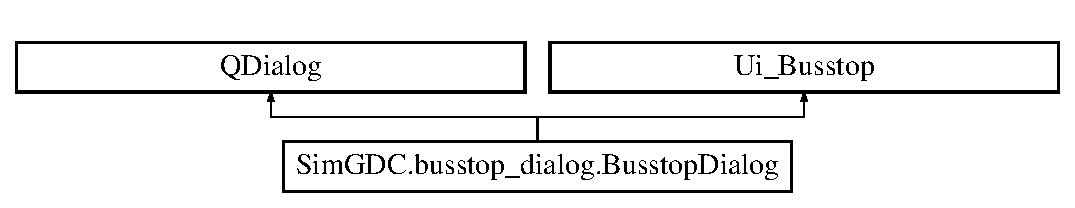
\includegraphics[height=2.000000cm]{class_sim_g_d_c_1_1busstop__dialog_1_1_busstop_dialog}
\end{center}
\end{figure}
\subsection*{Public Member Functions}
\begin{DoxyCompactItemize}
\item 
\hypertarget{class_sim_g_d_c_1_1busstop__dialog_1_1_busstop_dialog_add6ada42b492941baaa4a64d2824c88e}{}def {\bfseries \+\_\+\+\_\+init\+\_\+\+\_\+} (self)\label{class_sim_g_d_c_1_1busstop__dialog_1_1_busstop_dialog_add6ada42b492941baaa4a64d2824c88e}

\item 
\hypertarget{class_sim_g_d_c_1_1busstop__dialog_1_1_busstop_dialog_ab34a524ed0306eef6a54cee56e38ab5f}{}def {\bfseries get\+Segment\+List} (self)\label{class_sim_g_d_c_1_1busstop__dialog_1_1_busstop_dialog_ab34a524ed0306eef6a54cee56e38ab5f}

\item 
\hypertarget{class_sim_g_d_c_1_1busstop__dialog_1_1_busstop_dialog_a83c0f0d147b580c8eb77fc656681676d}{}def {\bfseries set\+Segment\+List} (self)\label{class_sim_g_d_c_1_1busstop__dialog_1_1_busstop_dialog_a83c0f0d147b580c8eb77fc656681676d}

\item 
\hypertarget{class_sim_g_d_c_1_1busstop__dialog_1_1_busstop_dialog_af2e09e20aedaa449cf2bdee9213044b3}{}def {\bfseries set\+Segment\+Id} (self, segment\+Id)\label{class_sim_g_d_c_1_1busstop__dialog_1_1_busstop_dialog_af2e09e20aedaa449cf2bdee9213044b3}

\item 
\hypertarget{class_sim_g_d_c_1_1busstop__dialog_1_1_busstop_dialog_ac1a464c1bff826e5b8d9fcfc8e363714}{}def {\bfseries addnewid} (self)\label{class_sim_g_d_c_1_1busstop__dialog_1_1_busstop_dialog_ac1a464c1bff826e5b8d9fcfc8e363714}

\item 
\hypertarget{class_sim_g_d_c_1_1busstop__dialog_1_1_busstop_dialog_a63637b2e310874b8fcd80f581d398a51}{}def {\bfseries calculate\+Offset} (self, point, segment\+Id)\label{class_sim_g_d_c_1_1busstop__dialog_1_1_busstop_dialog_a63637b2e310874b8fcd80f581d398a51}

\item 
\hypertarget{class_sim_g_d_c_1_1busstop__dialog_1_1_busstop_dialog_a918d4e1205671b2344a09718269760c6}{}def {\bfseries set\+Info} (self, info)\label{class_sim_g_d_c_1_1busstop__dialog_1_1_busstop_dialog_a918d4e1205671b2344a09718269760c6}

\item 
\hypertarget{class_sim_g_d_c_1_1busstop__dialog_1_1_busstop_dialog_a44a90ba7d93fe00457fa703c6c06999d}{}def {\bfseries update} (self)\label{class_sim_g_d_c_1_1busstop__dialog_1_1_busstop_dialog_a44a90ba7d93fe00457fa703c6c06999d}

\end{DoxyCompactItemize}
\subsection*{Public Attributes}
\begin{DoxyCompactItemize}
\item 
\hypertarget{class_sim_g_d_c_1_1busstop__dialog_1_1_busstop_dialog_a42b41009a757d93632f7ac474a5c618c}{}{\bfseries info}\label{class_sim_g_d_c_1_1busstop__dialog_1_1_busstop_dialog_a42b41009a757d93632f7ac474a5c618c}

\item 
\hypertarget{class_sim_g_d_c_1_1busstop__dialog_1_1_busstop_dialog_a3c1d7dbd66809968e6ad87ef6877d0ee}{}{\bfseries is\+Modified}\label{class_sim_g_d_c_1_1busstop__dialog_1_1_busstop_dialog_a3c1d7dbd66809968e6ad87ef6877d0ee}

\end{DoxyCompactItemize}
\subsection*{Static Public Attributes}
\begin{DoxyCompactItemize}
\item 
\hypertarget{class_sim_g_d_c_1_1busstop__dialog_1_1_busstop_dialog_a3534de4f0bfe51e37e5df51500759333}{}int {\bfseries original\+\_\+id} = 0\label{class_sim_g_d_c_1_1busstop__dialog_1_1_busstop_dialog_a3534de4f0bfe51e37e5df51500759333}

\end{DoxyCompactItemize}


The documentation for this class was generated from the following file\+:\begin{DoxyCompactItemize}
\item 
busstop\+\_\+dialog.\+py\end{DoxyCompactItemize}

\hypertarget{class_sim_g_d_c_1_1converter__dialog_1_1_converter_dialog}{}\section{Sim\+G\+D\+C.\+converter\+\_\+dialog.\+Converter\+Dialog Class Reference}
\label{class_sim_g_d_c_1_1converter__dialog_1_1_converter_dialog}\index{Sim\+G\+D\+C.\+converter\+\_\+dialog.\+Converter\+Dialog@{Sim\+G\+D\+C.\+converter\+\_\+dialog.\+Converter\+Dialog}}
Inheritance diagram for Sim\+G\+D\+C.\+converter\+\_\+dialog.\+Converter\+Dialog\+:\begin{figure}[H]
\begin{center}
\leavevmode
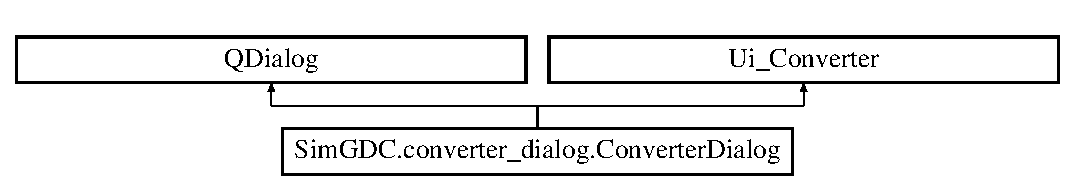
\includegraphics[height=2.000000cm]{class_sim_g_d_c_1_1converter__dialog_1_1_converter_dialog}
\end{center}
\end{figure}
\subsection*{Public Member Functions}
\begin{DoxyCompactItemize}
\item 
\hypertarget{class_sim_g_d_c_1_1converter__dialog_1_1_converter_dialog_accd1bb6154dacc08094656fd0cb13241}{}def {\bfseries \+\_\+\+\_\+init\+\_\+\+\_\+} (self)\label{class_sim_g_d_c_1_1converter__dialog_1_1_converter_dialog_accd1bb6154dacc08094656fd0cb13241}

\item 
\hypertarget{class_sim_g_d_c_1_1converter__dialog_1_1_converter_dialog_a8e40cd158db4ee2a201d73e7fbb09fa5}{}def {\bfseries xmlsh\+X\+M\+L\+Browser} (self)\label{class_sim_g_d_c_1_1converter__dialog_1_1_converter_dialog_a8e40cd158db4ee2a201d73e7fbb09fa5}

\item 
\hypertarget{class_sim_g_d_c_1_1converter__dialog_1_1_converter_dialog_ae5590da2bfec49058a9ca244a45bdd5f}{}def {\bfseries shxml\+X\+M\+L\+Browser} (self)\label{class_sim_g_d_c_1_1converter__dialog_1_1_converter_dialog_ae5590da2bfec49058a9ca244a45bdd5f}

\item 
\hypertarget{class_sim_g_d_c_1_1converter__dialog_1_1_converter_dialog_a770533270053d19ec4aa00c7bfd1dcbb}{}def {\bfseries xmlsh\+S\+H\+Browser} (self)\label{class_sim_g_d_c_1_1converter__dialog_1_1_converter_dialog_a770533270053d19ec4aa00c7bfd1dcbb}

\item 
\hypertarget{class_sim_g_d_c_1_1converter__dialog_1_1_converter_dialog_a3fae55c205ff7089ea31c1976d4220be}{}def {\bfseries shxml\+S\+H\+Browser} (self)\label{class_sim_g_d_c_1_1converter__dialog_1_1_converter_dialog_a3fae55c205ff7089ea31c1976d4220be}

\item 
\hypertarget{class_sim_g_d_c_1_1converter__dialog_1_1_converter_dialog_a3c6abc9532c4fb7f1ae5fe2f3da3ede7}{}def {\bfseries xmlsh\+Update\+Progress} (self, value)\label{class_sim_g_d_c_1_1converter__dialog_1_1_converter_dialog_a3c6abc9532c4fb7f1ae5fe2f3da3ede7}

\item 
\hypertarget{class_sim_g_d_c_1_1converter__dialog_1_1_converter_dialog_ac8dee43228e575ec978940f25c4d956e}{}def {\bfseries shxml\+Update\+Progress} (self, value)\label{class_sim_g_d_c_1_1converter__dialog_1_1_converter_dialog_ac8dee43228e575ec978940f25c4d956e}

\item 
\hypertarget{class_sim_g_d_c_1_1converter__dialog_1_1_converter_dialog_a884838f4da1c8411c4464da50512827b}{}def {\bfseries convert\+X\+M\+L\+To\+S\+H} (self)\label{class_sim_g_d_c_1_1converter__dialog_1_1_converter_dialog_a884838f4da1c8411c4464da50512827b}

\item 
\hypertarget{class_sim_g_d_c_1_1converter__dialog_1_1_converter_dialog_ad956e1d566a415ecf2f37aa11257df10}{}def {\bfseries convert\+S\+H\+To\+X\+M\+L} (self)\label{class_sim_g_d_c_1_1converter__dialog_1_1_converter_dialog_ad956e1d566a415ecf2f37aa11257df10}

\end{DoxyCompactItemize}
\subsection*{Static Public Attributes}
\begin{DoxyCompactItemize}
\item 
\hypertarget{class_sim_g_d_c_1_1converter__dialog_1_1_converter_dialog_af65905920c6fa8afb9e489ac7a04e383}{}tuple {\bfseries open\+\_\+sig} = Qt\+Core.\+pyqt\+Signal(str)\label{class_sim_g_d_c_1_1converter__dialog_1_1_converter_dialog_af65905920c6fa8afb9e489ac7a04e383}

\end{DoxyCompactItemize}


The documentation for this class was generated from the following file\+:\begin{DoxyCompactItemize}
\item 
converter\+\_\+dialog.\+py\end{DoxyCompactItemize}

\hypertarget{class_sim_g_d_c_1_1crossing__dialog_1_1_crossing_dialog}{}\section{Sim\+G\+D\+C.\+crossing\+\_\+dialog.\+Crossing\+Dialog Class Reference}
\label{class_sim_g_d_c_1_1crossing__dialog_1_1_crossing_dialog}\index{Sim\+G\+D\+C.\+crossing\+\_\+dialog.\+Crossing\+Dialog@{Sim\+G\+D\+C.\+crossing\+\_\+dialog.\+Crossing\+Dialog}}
Inheritance diagram for Sim\+G\+D\+C.\+crossing\+\_\+dialog.\+Crossing\+Dialog\+:\begin{figure}[H]
\begin{center}
\leavevmode
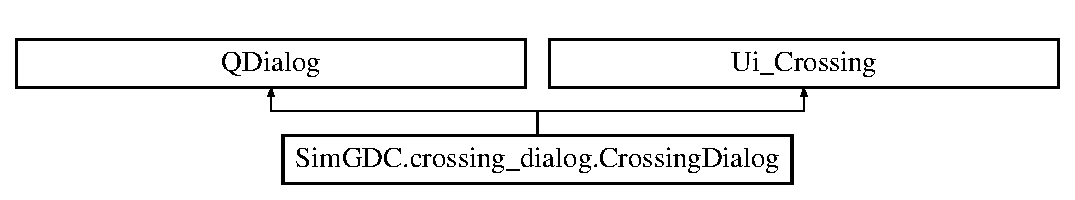
\includegraphics[height=2.000000cm]{class_sim_g_d_c_1_1crossing__dialog_1_1_crossing_dialog}
\end{center}
\end{figure}
\subsection*{Public Member Functions}
\begin{DoxyCompactItemize}
\item 
\hypertarget{class_sim_g_d_c_1_1crossing__dialog_1_1_crossing_dialog_abbbfbbae8f4ffc477748ca3f78622b04}{}def {\bfseries \+\_\+\+\_\+init\+\_\+\+\_\+} (self)\label{class_sim_g_d_c_1_1crossing__dialog_1_1_crossing_dialog_abbbfbbae8f4ffc477748ca3f78622b04}

\item 
\hypertarget{class_sim_g_d_c_1_1crossing__dialog_1_1_crossing_dialog_aa483443e4bf64167f777c8ff55474bf9}{}def {\bfseries set\+Segment\+Id} (self, segment\+Id)\label{class_sim_g_d_c_1_1crossing__dialog_1_1_crossing_dialog_aa483443e4bf64167f777c8ff55474bf9}

\item 
\hypertarget{class_sim_g_d_c_1_1crossing__dialog_1_1_crossing_dialog_a027c3eb85ab0ee8091895b73aa28b546}{}def {\bfseries set\+Info} (self, info)\label{class_sim_g_d_c_1_1crossing__dialog_1_1_crossing_dialog_a027c3eb85ab0ee8091895b73aa28b546}

\item 
\hypertarget{class_sim_g_d_c_1_1crossing__dialog_1_1_crossing_dialog_ae5fede343a9e0ae3f0ff634a7273bb0f}{}def {\bfseries update} (self)\label{class_sim_g_d_c_1_1crossing__dialog_1_1_crossing_dialog_ae5fede343a9e0ae3f0ff634a7273bb0f}

\end{DoxyCompactItemize}
\subsection*{Public Attributes}
\begin{DoxyCompactItemize}
\item 
\hypertarget{class_sim_g_d_c_1_1crossing__dialog_1_1_crossing_dialog_a580203ae3b823d38f53ecad1896daf3b}{}{\bfseries info}\label{class_sim_g_d_c_1_1crossing__dialog_1_1_crossing_dialog_a580203ae3b823d38f53ecad1896daf3b}

\item 
\hypertarget{class_sim_g_d_c_1_1crossing__dialog_1_1_crossing_dialog_a75f2b60cd5702a7a7cc79f8df4a746ad}{}{\bfseries is\+Modified}\label{class_sim_g_d_c_1_1crossing__dialog_1_1_crossing_dialog_a75f2b60cd5702a7a7cc79f8df4a746ad}

\end{DoxyCompactItemize}


The documentation for this class was generated from the following file\+:\begin{DoxyCompactItemize}
\item 
crossing\+\_\+dialog.\+py\end{DoxyCompactItemize}

\hypertarget{class_sim_g_d_c_1_1lane__dialog_1_1_lane_dialog}{}\section{Sim\+G\+D\+C.\+lane\+\_\+dialog.\+Lane\+Dialog Class Reference}
\label{class_sim_g_d_c_1_1lane__dialog_1_1_lane_dialog}\index{Sim\+G\+D\+C.\+lane\+\_\+dialog.\+Lane\+Dialog@{Sim\+G\+D\+C.\+lane\+\_\+dialog.\+Lane\+Dialog}}
Inheritance diagram for Sim\+G\+D\+C.\+lane\+\_\+dialog.\+Lane\+Dialog\+:\begin{figure}[H]
\begin{center}
\leavevmode
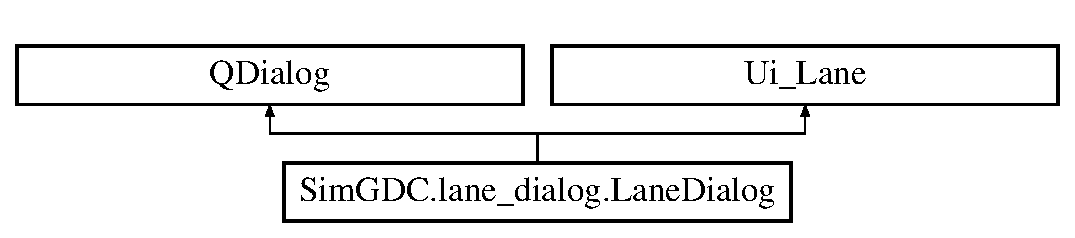
\includegraphics[height=2.000000cm]{class_sim_g_d_c_1_1lane__dialog_1_1_lane_dialog}
\end{center}
\end{figure}
\subsection*{Public Member Functions}
\begin{DoxyCompactItemize}
\item 
\hypertarget{class_sim_g_d_c_1_1lane__dialog_1_1_lane_dialog_aeb304a5b202091a7d47a8dfe4eed568f}{}def {\bfseries \+\_\+\+\_\+init\+\_\+\+\_\+} (self)\label{class_sim_g_d_c_1_1lane__dialog_1_1_lane_dialog_aeb304a5b202091a7d47a8dfe4eed568f}

\item 
\hypertarget{class_sim_g_d_c_1_1lane__dialog_1_1_lane_dialog_a55f9d46bbdc9c94c97af4fbab82cfc73}{}def {\bfseries set\+Segment\+Id} (self, segment\+Id)\label{class_sim_g_d_c_1_1lane__dialog_1_1_lane_dialog_a55f9d46bbdc9c94c97af4fbab82cfc73}

\item 
\hypertarget{class_sim_g_d_c_1_1lane__dialog_1_1_lane_dialog_a3aae9751e93d910fda7e8bd4c448ecff}{}def {\bfseries set\+Info} (self, info)\label{class_sim_g_d_c_1_1lane__dialog_1_1_lane_dialog_a3aae9751e93d910fda7e8bd4c448ecff}

\item 
\hypertarget{class_sim_g_d_c_1_1lane__dialog_1_1_lane_dialog_af0e98a74b33bb5dac28a99ca50a947c9}{}def {\bfseries update} (self)\label{class_sim_g_d_c_1_1lane__dialog_1_1_lane_dialog_af0e98a74b33bb5dac28a99ca50a947c9}

\end{DoxyCompactItemize}
\subsection*{Public Attributes}
\begin{DoxyCompactItemize}
\item 
\hypertarget{class_sim_g_d_c_1_1lane__dialog_1_1_lane_dialog_a64bc913ea31aa3c1525e71dccf3eeb29}{}{\bfseries info}\label{class_sim_g_d_c_1_1lane__dialog_1_1_lane_dialog_a64bc913ea31aa3c1525e71dccf3eeb29}

\item 
\hypertarget{class_sim_g_d_c_1_1lane__dialog_1_1_lane_dialog_a12aaa8f8669db94cc9dfca47f59fcc96}{}{\bfseries is\+Modified}\label{class_sim_g_d_c_1_1lane__dialog_1_1_lane_dialog_a12aaa8f8669db94cc9dfca47f59fcc96}

\end{DoxyCompactItemize}


The documentation for this class was generated from the following file\+:\begin{DoxyCompactItemize}
\item 
lane\+\_\+dialog.\+py\end{DoxyCompactItemize}

\hypertarget{class_sim_g_d_c_1_1laneedge__dialog_1_1_lane_edge_dialog}{}\section{Sim\+G\+D\+C.\+laneedge\+\_\+dialog.\+Lane\+Edge\+Dialog Class Reference}
\label{class_sim_g_d_c_1_1laneedge__dialog_1_1_lane_edge_dialog}\index{Sim\+G\+D\+C.\+laneedge\+\_\+dialog.\+Lane\+Edge\+Dialog@{Sim\+G\+D\+C.\+laneedge\+\_\+dialog.\+Lane\+Edge\+Dialog}}
Inheritance diagram for Sim\+G\+D\+C.\+laneedge\+\_\+dialog.\+Lane\+Edge\+Dialog\+:\begin{figure}[H]
\begin{center}
\leavevmode
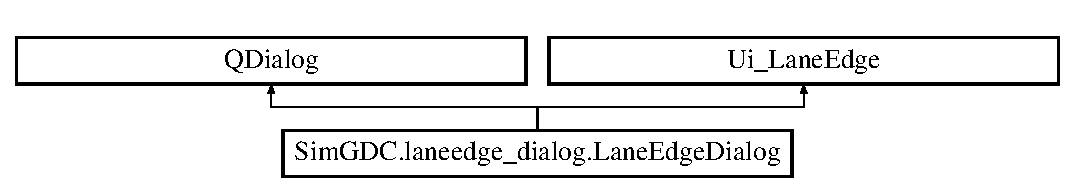
\includegraphics[height=2.000000cm]{class_sim_g_d_c_1_1laneedge__dialog_1_1_lane_edge_dialog}
\end{center}
\end{figure}
\subsection*{Public Member Functions}
\begin{DoxyCompactItemize}
\item 
\hypertarget{class_sim_g_d_c_1_1laneedge__dialog_1_1_lane_edge_dialog_a8775606b9df2579d07d1a611c8284124}{}def {\bfseries \+\_\+\+\_\+init\+\_\+\+\_\+} (self)\label{class_sim_g_d_c_1_1laneedge__dialog_1_1_lane_edge_dialog_a8775606b9df2579d07d1a611c8284124}

\item 
\hypertarget{class_sim_g_d_c_1_1laneedge__dialog_1_1_lane_edge_dialog_ae6a1a5b36a2aa2aff346029806b97070}{}def {\bfseries set\+Segment\+Id} (self, segment\+Id)\label{class_sim_g_d_c_1_1laneedge__dialog_1_1_lane_edge_dialog_ae6a1a5b36a2aa2aff346029806b97070}

\item 
\hypertarget{class_sim_g_d_c_1_1laneedge__dialog_1_1_lane_edge_dialog_a8b790c749a613ec62f44640e7be41508}{}def {\bfseries set\+Info} (self, info)\label{class_sim_g_d_c_1_1laneedge__dialog_1_1_lane_edge_dialog_a8b790c749a613ec62f44640e7be41508}

\item 
\hypertarget{class_sim_g_d_c_1_1laneedge__dialog_1_1_lane_edge_dialog_adc18f9b100e707b73ad11ae57af9a069}{}def {\bfseries update} (self)\label{class_sim_g_d_c_1_1laneedge__dialog_1_1_lane_edge_dialog_adc18f9b100e707b73ad11ae57af9a069}

\end{DoxyCompactItemize}
\subsection*{Public Attributes}
\begin{DoxyCompactItemize}
\item 
\hypertarget{class_sim_g_d_c_1_1laneedge__dialog_1_1_lane_edge_dialog_afca596b47d84bf9a1d7f65e2bd5b81e5}{}{\bfseries info}\label{class_sim_g_d_c_1_1laneedge__dialog_1_1_lane_edge_dialog_afca596b47d84bf9a1d7f65e2bd5b81e5}

\item 
\hypertarget{class_sim_g_d_c_1_1laneedge__dialog_1_1_lane_edge_dialog_a2f521fbd28ef7e45cefa2e46f15e55d1}{}{\bfseries is\+Modified}\label{class_sim_g_d_c_1_1laneedge__dialog_1_1_lane_edge_dialog_a2f521fbd28ef7e45cefa2e46f15e55d1}

\end{DoxyCompactItemize}


The documentation for this class was generated from the following file\+:\begin{DoxyCompactItemize}
\item 
laneedge\+\_\+dialog.\+py\end{DoxyCompactItemize}

\hypertarget{class_sim_g_d_c_1_1linkmanager__dialog_1_1_link_manager_dialog}{}\section{Sim\+G\+D\+C.\+linkmanager\+\_\+dialog.\+Link\+Manager\+Dialog Class Reference}
\label{class_sim_g_d_c_1_1linkmanager__dialog_1_1_link_manager_dialog}\index{Sim\+G\+D\+C.\+linkmanager\+\_\+dialog.\+Link\+Manager\+Dialog@{Sim\+G\+D\+C.\+linkmanager\+\_\+dialog.\+Link\+Manager\+Dialog}}
Inheritance diagram for Sim\+G\+D\+C.\+linkmanager\+\_\+dialog.\+Link\+Manager\+Dialog\+:\begin{figure}[H]
\begin{center}
\leavevmode
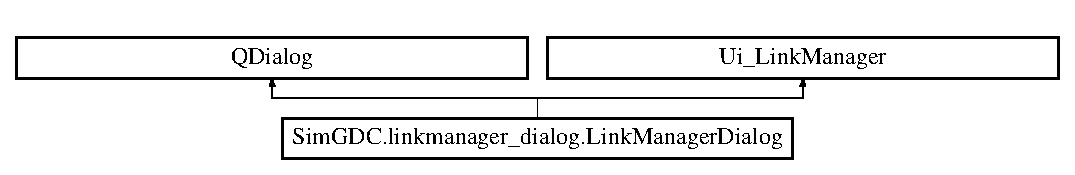
\includegraphics[height=1.904762cm]{class_sim_g_d_c_1_1linkmanager__dialog_1_1_link_manager_dialog}
\end{center}
\end{figure}
\subsection*{Public Member Functions}
\begin{DoxyCompactItemize}
\item 
\hypertarget{class_sim_g_d_c_1_1linkmanager__dialog_1_1_link_manager_dialog_a7e356813ab9967d3b200cc03f16837db}{}def {\bfseries \+\_\+\+\_\+init\+\_\+\+\_\+} (self)\label{class_sim_g_d_c_1_1linkmanager__dialog_1_1_link_manager_dialog_a7e356813ab9967d3b200cc03f16837db}

\item 
\hypertarget{class_sim_g_d_c_1_1linkmanager__dialog_1_1_link_manager_dialog_ace0f8593497078e32ceb45e7b7d9945c}{}def {\bfseries set\+Link\+List} (self, links)\label{class_sim_g_d_c_1_1linkmanager__dialog_1_1_link_manager_dialog_ace0f8593497078e32ceb45e7b7d9945c}

\item 
\hypertarget{class_sim_g_d_c_1_1linkmanager__dialog_1_1_link_manager_dialog_a6d279ba70974667679a546be721ce245}{}def {\bfseries set\+Node\+List} (self)\label{class_sim_g_d_c_1_1linkmanager__dialog_1_1_link_manager_dialog_a6d279ba70974667679a546be721ce245}

\item 
\hypertarget{class_sim_g_d_c_1_1linkmanager__dialog_1_1_link_manager_dialog_a2cc05733990f9e403a89add722b9ea23}{}def {\bfseries update\+Link\+Name} (self, text\+Link\+Id)\label{class_sim_g_d_c_1_1linkmanager__dialog_1_1_link_manager_dialog_a2cc05733990f9e403a89add722b9ea23}

\item 
\hypertarget{class_sim_g_d_c_1_1linkmanager__dialog_1_1_link_manager_dialog_afd15b0210bbc194771e9f03981fc3055}{}def {\bfseries addnewid} (self)\label{class_sim_g_d_c_1_1linkmanager__dialog_1_1_link_manager_dialog_afd15b0210bbc194771e9f03981fc3055}

\item 
\hypertarget{class_sim_g_d_c_1_1linkmanager__dialog_1_1_link_manager_dialog_a3037f99b8bed297359b21f60e9641ee4}{}def {\bfseries update} (self)\label{class_sim_g_d_c_1_1linkmanager__dialog_1_1_link_manager_dialog_a3037f99b8bed297359b21f60e9641ee4}

\end{DoxyCompactItemize}
\subsection*{Public Attributes}
\begin{DoxyCompactItemize}
\item 
\hypertarget{class_sim_g_d_c_1_1linkmanager__dialog_1_1_link_manager_dialog_ac4266a788b7474cdee91753d652cf01e}{}{\bfseries info}\label{class_sim_g_d_c_1_1linkmanager__dialog_1_1_link_manager_dialog_ac4266a788b7474cdee91753d652cf01e}

\item 
\hypertarget{class_sim_g_d_c_1_1linkmanager__dialog_1_1_link_manager_dialog_a733bc96c3cf5fb10ed399018eff966d7}{}{\bfseries list\+Links}\label{class_sim_g_d_c_1_1linkmanager__dialog_1_1_link_manager_dialog_a733bc96c3cf5fb10ed399018eff966d7}

\item 
\hypertarget{class_sim_g_d_c_1_1linkmanager__dialog_1_1_link_manager_dialog_ad295d74c12ccdf731f263320dcaea77e}{}{\bfseries is\+Modified}\label{class_sim_g_d_c_1_1linkmanager__dialog_1_1_link_manager_dialog_ad295d74c12ccdf731f263320dcaea77e}

\item 
\hypertarget{class_sim_g_d_c_1_1linkmanager__dialog_1_1_link_manager_dialog_ae5659410a38ee189239ea4dc4a6dd0c2}{}{\bfseries node\+List}\label{class_sim_g_d_c_1_1linkmanager__dialog_1_1_link_manager_dialog_ae5659410a38ee189239ea4dc4a6dd0c2}

\end{DoxyCompactItemize}


The documentation for this class was generated from the following file\+:\begin{DoxyCompactItemize}
\item 
linkmanager\+\_\+dialog.\+py\end{DoxyCompactItemize}

\hypertarget{class_sim_g_d_c_1_1multinode__dialog_1_1_multi_node_dialog}{}\section{Sim\+G\+D\+C.\+multinode\+\_\+dialog.\+Multi\+Node\+Dialog Class Reference}
\label{class_sim_g_d_c_1_1multinode__dialog_1_1_multi_node_dialog}\index{Sim\+G\+D\+C.\+multinode\+\_\+dialog.\+Multi\+Node\+Dialog@{Sim\+G\+D\+C.\+multinode\+\_\+dialog.\+Multi\+Node\+Dialog}}
Inheritance diagram for Sim\+G\+D\+C.\+multinode\+\_\+dialog.\+Multi\+Node\+Dialog\+:\begin{figure}[H]
\begin{center}
\leavevmode
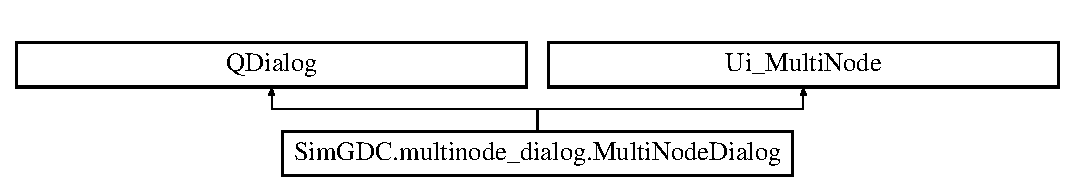
\includegraphics[height=2.000000cm]{class_sim_g_d_c_1_1multinode__dialog_1_1_multi_node_dialog}
\end{center}
\end{figure}
\subsection*{Public Member Functions}
\begin{DoxyCompactItemize}
\item 
\hypertarget{class_sim_g_d_c_1_1multinode__dialog_1_1_multi_node_dialog_a4d09eac4617f3a947484ecb5511ec78c}{}def {\bfseries \+\_\+\+\_\+init\+\_\+\+\_\+} (self)\label{class_sim_g_d_c_1_1multinode__dialog_1_1_multi_node_dialog_a4d09eac4617f3a947484ecb5511ec78c}

\item 
\hypertarget{class_sim_g_d_c_1_1multinode__dialog_1_1_multi_node_dialog_ab1a57d1c144ff1e449f51a29c4f0db31}{}def {\bfseries set\+Info} (self, info)\label{class_sim_g_d_c_1_1multinode__dialog_1_1_multi_node_dialog_ab1a57d1c144ff1e449f51a29c4f0db31}

\item 
\hypertarget{class_sim_g_d_c_1_1multinode__dialog_1_1_multi_node_dialog_ac92cc73cbff50710e3c890dae39768e8}{}def {\bfseries add\+Turning\+Group} (self)\label{class_sim_g_d_c_1_1multinode__dialog_1_1_multi_node_dialog_ac92cc73cbff50710e3c890dae39768e8}

\item 
\hypertarget{class_sim_g_d_c_1_1multinode__dialog_1_1_multi_node_dialog_a9d39737ee0e9aa99a1d329b4af38ace3}{}def {\bfseries add\+Turning\+Path} (self)\label{class_sim_g_d_c_1_1multinode__dialog_1_1_multi_node_dialog_a9d39737ee0e9aa99a1d329b4af38ace3}

\item 
\hypertarget{class_sim_g_d_c_1_1multinode__dialog_1_1_multi_node_dialog_a228d2b49d218d0b56722a52c89571b10}{}def {\bfseries displayturninggroup} (self)\label{class_sim_g_d_c_1_1multinode__dialog_1_1_multi_node_dialog_a228d2b49d218d0b56722a52c89571b10}

\item 
\hypertarget{class_sim_g_d_c_1_1multinode__dialog_1_1_multi_node_dialog_a1d6f99acf7071edfb11958dc3eff5a0c}{}def {\bfseries displayturningpath} (self)\label{class_sim_g_d_c_1_1multinode__dialog_1_1_multi_node_dialog_a1d6f99acf7071edfb11958dc3eff5a0c}

\item 
\hypertarget{class_sim_g_d_c_1_1multinode__dialog_1_1_multi_node_dialog_a26530213037eadf247b3c503f5c47eb8}{}def {\bfseries set\+Linklist} (self)\label{class_sim_g_d_c_1_1multinode__dialog_1_1_multi_node_dialog_a26530213037eadf247b3c503f5c47eb8}

\item 
\hypertarget{class_sim_g_d_c_1_1multinode__dialog_1_1_multi_node_dialog_aa68775c544c257e69724e0899e16a2ce}{}def {\bfseries set\+Lanelist} (self)\label{class_sim_g_d_c_1_1multinode__dialog_1_1_multi_node_dialog_aa68775c544c257e69724e0899e16a2ce}

\item 
\hypertarget{class_sim_g_d_c_1_1multinode__dialog_1_1_multi_node_dialog_a8a8b6f446b8551b6d6f7ef2b49c8d18e}{}def {\bfseries addnewid} (self)\label{class_sim_g_d_c_1_1multinode__dialog_1_1_multi_node_dialog_a8a8b6f446b8551b6d6f7ef2b49c8d18e}

\item 
\hypertarget{class_sim_g_d_c_1_1multinode__dialog_1_1_multi_node_dialog_a80c989a436a01c5421ecda309dc43b14}{}def {\bfseries delete\+Turning\+Group} (self)\label{class_sim_g_d_c_1_1multinode__dialog_1_1_multi_node_dialog_a80c989a436a01c5421ecda309dc43b14}

\item 
\hypertarget{class_sim_g_d_c_1_1multinode__dialog_1_1_multi_node_dialog_a3cc78bec5da9a0acb3c45d94dafb1ee0}{}def {\bfseries delete\+Turning\+Path} (self)\label{class_sim_g_d_c_1_1multinode__dialog_1_1_multi_node_dialog_a3cc78bec5da9a0acb3c45d94dafb1ee0}

\item 
\hypertarget{class_sim_g_d_c_1_1multinode__dialog_1_1_multi_node_dialog_abf18de57b521f7af1132e5b5b249ec84}{}def {\bfseries update} (self)\label{class_sim_g_d_c_1_1multinode__dialog_1_1_multi_node_dialog_abf18de57b521f7af1132e5b5b249ec84}

\end{DoxyCompactItemize}
\subsection*{Public Attributes}
\begin{DoxyCompactItemize}
\item 
\hypertarget{class_sim_g_d_c_1_1multinode__dialog_1_1_multi_node_dialog_a903c390d20bad360e2bedbbbbf2cf720}{}{\bfseries info}\label{class_sim_g_d_c_1_1multinode__dialog_1_1_multi_node_dialog_a903c390d20bad360e2bedbbbbf2cf720}

\item 
\hypertarget{class_sim_g_d_c_1_1multinode__dialog_1_1_multi_node_dialog_a194eb8e560e224b45a72303af4c6ad50}{}{\bfseries is\+Modified}\label{class_sim_g_d_c_1_1multinode__dialog_1_1_multi_node_dialog_a194eb8e560e224b45a72303af4c6ad50}

\item 
\hypertarget{class_sim_g_d_c_1_1multinode__dialog_1_1_multi_node_dialog_add2237c73b1cba300ee0b26f07f48bef}{}{\bfseries list\+Segments}\label{class_sim_g_d_c_1_1multinode__dialog_1_1_multi_node_dialog_add2237c73b1cba300ee0b26f07f48bef}

\end{DoxyCompactItemize}
\subsection*{Static Public Attributes}
\begin{DoxyCompactItemize}
\item 
\hypertarget{class_sim_g_d_c_1_1multinode__dialog_1_1_multi_node_dialog_afb77dcb09741ec2ecac5a9bd863a6742}{}int {\bfseries original\+\_\+id} = 0\label{class_sim_g_d_c_1_1multinode__dialog_1_1_multi_node_dialog_afb77dcb09741ec2ecac5a9bd863a6742}

\end{DoxyCompactItemize}


The documentation for this class was generated from the following file\+:\begin{DoxyCompactItemize}
\item 
multinode\+\_\+dialog.\+py\end{DoxyCompactItemize}

\hypertarget{class_sim_g_d_c_1_1segment__dialog_1_1_segment_dialog}{}\section{Sim\+G\+D\+C.\+segment\+\_\+dialog.\+Segment\+Dialog Class Reference}
\label{class_sim_g_d_c_1_1segment__dialog_1_1_segment_dialog}\index{Sim\+G\+D\+C.\+segment\+\_\+dialog.\+Segment\+Dialog@{Sim\+G\+D\+C.\+segment\+\_\+dialog.\+Segment\+Dialog}}
Inheritance diagram for Sim\+G\+D\+C.\+segment\+\_\+dialog.\+Segment\+Dialog\+:\begin{figure}[H]
\begin{center}
\leavevmode
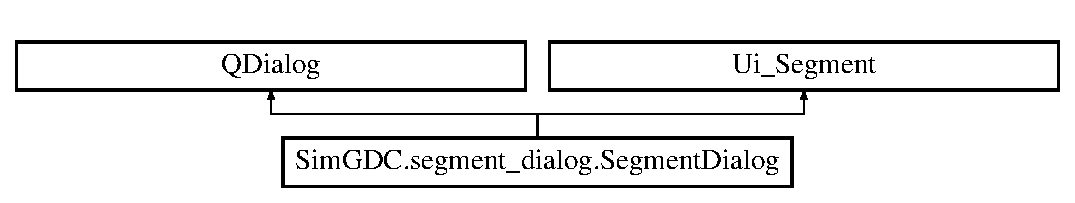
\includegraphics[height=2.000000cm]{class_sim_g_d_c_1_1segment__dialog_1_1_segment_dialog}
\end{center}
\end{figure}
\subsection*{Public Member Functions}
\begin{DoxyCompactItemize}
\item 
\hypertarget{class_sim_g_d_c_1_1segment__dialog_1_1_segment_dialog_a6d2d1e65938f0e457622d5c77f4eeed6}{}def {\bfseries \+\_\+\+\_\+init\+\_\+\+\_\+} (self)\label{class_sim_g_d_c_1_1segment__dialog_1_1_segment_dialog_a6d2d1e65938f0e457622d5c77f4eeed6}

\item 
\hypertarget{class_sim_g_d_c_1_1segment__dialog_1_1_segment_dialog_a6ff94b6ac03c2ae607ee6a536130f2ba}{}def {\bfseries set\+Link\+List} (self, links)\label{class_sim_g_d_c_1_1segment__dialog_1_1_segment_dialog_a6ff94b6ac03c2ae607ee6a536130f2ba}

\item 
\hypertarget{class_sim_g_d_c_1_1segment__dialog_1_1_segment_dialog_aea8548ca0c8efa08afe8c91a51b77b59}{}def {\bfseries set\+Info} (self, info)\label{class_sim_g_d_c_1_1segment__dialog_1_1_segment_dialog_aea8548ca0c8efa08afe8c91a51b77b59}

\item 
\hypertarget{class_sim_g_d_c_1_1segment__dialog_1_1_segment_dialog_a3ffe71d0c9c6df5248682cdfd07f2aab}{}def {\bfseries deleteconnector} (self)\label{class_sim_g_d_c_1_1segment__dialog_1_1_segment_dialog_a3ffe71d0c9c6df5248682cdfd07f2aab}

\item 
\hypertarget{class_sim_g_d_c_1_1segment__dialog_1_1_segment_dialog_a254c29e8d53ae58fa2b06f2c9d3739e1}{}def {\bfseries addnewid} (self)\label{class_sim_g_d_c_1_1segment__dialog_1_1_segment_dialog_a254c29e8d53ae58fa2b06f2c9d3739e1}

\item 
\hypertarget{class_sim_g_d_c_1_1segment__dialog_1_1_segment_dialog_a35be203621a2a474c0b72fee30baba62}{}def {\bfseries addlaneconnector} (self)\label{class_sim_g_d_c_1_1segment__dialog_1_1_segment_dialog_a35be203621a2a474c0b72fee30baba62}

\item 
\hypertarget{class_sim_g_d_c_1_1segment__dialog_1_1_segment_dialog_a2c6530c15d945c7c41839d0c6a81a770}{}def {\bfseries displayconnector} (self)\label{class_sim_g_d_c_1_1segment__dialog_1_1_segment_dialog_a2c6530c15d945c7c41839d0c6a81a770}

\item 
\hypertarget{class_sim_g_d_c_1_1segment__dialog_1_1_segment_dialog_a81f05bc0d00d09cc57164da789e8263f}{}def {\bfseries update} (self)\label{class_sim_g_d_c_1_1segment__dialog_1_1_segment_dialog_a81f05bc0d00d09cc57164da789e8263f}

\end{DoxyCompactItemize}
\subsection*{Public Attributes}
\begin{DoxyCompactItemize}
\item 
\hypertarget{class_sim_g_d_c_1_1segment__dialog_1_1_segment_dialog_a96bd24afac6e0bbe351807e5fb9210ed}{}{\bfseries info}\label{class_sim_g_d_c_1_1segment__dialog_1_1_segment_dialog_a96bd24afac6e0bbe351807e5fb9210ed}

\item 
\hypertarget{class_sim_g_d_c_1_1segment__dialog_1_1_segment_dialog_a4a09903d04e82e83ff0f02916cf3289a}{}{\bfseries list\+Links}\label{class_sim_g_d_c_1_1segment__dialog_1_1_segment_dialog_a4a09903d04e82e83ff0f02916cf3289a}

\item 
\hypertarget{class_sim_g_d_c_1_1segment__dialog_1_1_segment_dialog_aa58d6ec9b8afd33faa93902a8e74fde6}{}{\bfseries is\+Modified}\label{class_sim_g_d_c_1_1segment__dialog_1_1_segment_dialog_aa58d6ec9b8afd33faa93902a8e74fde6}

\item 
\hypertarget{class_sim_g_d_c_1_1segment__dialog_1_1_segment_dialog_a3620ae05efa6a97aa76cc1dc364b0b88}{}{\bfseries laneconnectorlist}\label{class_sim_g_d_c_1_1segment__dialog_1_1_segment_dialog_a3620ae05efa6a97aa76cc1dc364b0b88}

\end{DoxyCompactItemize}
\subsection*{Static Public Attributes}
\begin{DoxyCompactItemize}
\item 
\hypertarget{class_sim_g_d_c_1_1segment__dialog_1_1_segment_dialog_aa516c418b1814a56e0c0a3111d9d3546}{}int {\bfseries original\+\_\+id} = 0\label{class_sim_g_d_c_1_1segment__dialog_1_1_segment_dialog_aa516c418b1814a56e0c0a3111d9d3546}

\end{DoxyCompactItemize}


The documentation for this class was generated from the following file\+:\begin{DoxyCompactItemize}
\item 
segment\+\_\+dialog.\+py\end{DoxyCompactItemize}

\hypertarget{class_sim_g_d_c_1_1shapefile_i_o_1_1_shapefile_reader}{}\section{Sim\+G\+D\+C.\+shapefile\+I\+O.\+Shapefile\+Reader Class Reference}
\label{class_sim_g_d_c_1_1shapefile_i_o_1_1_shapefile_reader}\index{Sim\+G\+D\+C.\+shapefile\+I\+O.\+Shapefile\+Reader@{Sim\+G\+D\+C.\+shapefile\+I\+O.\+Shapefile\+Reader}}
\subsection*{Public Member Functions}
\begin{DoxyCompactItemize}
\item 
\hypertarget{class_sim_g_d_c_1_1shapefile_i_o_1_1_shapefile_reader_a4ac8c5604c3c9f3b6ead3e67996ca77f}{}def {\bfseries \+\_\+\+\_\+init\+\_\+\+\_\+} (self, path)\label{class_sim_g_d_c_1_1shapefile_i_o_1_1_shapefile_reader_a4ac8c5604c3c9f3b6ead3e67996ca77f}

\item 
\hypertarget{class_sim_g_d_c_1_1shapefile_i_o_1_1_shapefile_reader_ad69dd3eac5e87f5260d5e3c53c17aebc}{}def {\bfseries load\+Data} (self, typeid)\label{class_sim_g_d_c_1_1shapefile_i_o_1_1_shapefile_reader_ad69dd3eac5e87f5260d5e3c53c17aebc}

\item 
\hypertarget{class_sim_g_d_c_1_1shapefile_i_o_1_1_shapefile_reader_a8e15a35f330665afb7f75670a51b472c}{}def {\bfseries get\+Nodes} (self, type\+Id)\label{class_sim_g_d_c_1_1shapefile_i_o_1_1_shapefile_reader_a8e15a35f330665afb7f75670a51b472c}

\item 
\hypertarget{class_sim_g_d_c_1_1shapefile_i_o_1_1_shapefile_reader_a7a92357d019f1635e39e4a2e2828354b}{}def {\bfseries get\+Segments\+By\+Link\+Id} (self, link\+Id)\label{class_sim_g_d_c_1_1shapefile_i_o_1_1_shapefile_reader_a7a92357d019f1635e39e4a2e2828354b}

\item 
\hypertarget{class_sim_g_d_c_1_1shapefile_i_o_1_1_shapefile_reader_a53512a2289e336f116b4d113b0f5d5fe}{}def {\bfseries get\+Segment\+Components} (self, type\+Id, segment\+Id)\label{class_sim_g_d_c_1_1shapefile_i_o_1_1_shapefile_reader_a53512a2289e336f116b4d113b0f5d5fe}

\end{DoxyCompactItemize}
\subsection*{Public Attributes}
\begin{DoxyCompactItemize}
\item 
\hypertarget{class_sim_g_d_c_1_1shapefile_i_o_1_1_shapefile_reader_afc7c5d2dcabc49ec05431c069872dc25}{}{\bfseries path}\label{class_sim_g_d_c_1_1shapefile_i_o_1_1_shapefile_reader_afc7c5d2dcabc49ec05431c069872dc25}

\item 
\hypertarget{class_sim_g_d_c_1_1shapefile_i_o_1_1_shapefile_reader_a39a239ebe8e9515d3e840763276b0757}{}{\bfseries prefix}\label{class_sim_g_d_c_1_1shapefile_i_o_1_1_shapefile_reader_a39a239ebe8e9515d3e840763276b0757}

\item 
\hypertarget{class_sim_g_d_c_1_1shapefile_i_o_1_1_shapefile_reader_a06978d3e54e8cc53a881238c41653ca9}{}{\bfseries layer}\label{class_sim_g_d_c_1_1shapefile_i_o_1_1_shapefile_reader_a06978d3e54e8cc53a881238c41653ca9}

\item 
\hypertarget{class_sim_g_d_c_1_1shapefile_i_o_1_1_shapefile_reader_af5bc9055f89c0b8510609213039016b9}{}{\bfseries data}\label{class_sim_g_d_c_1_1shapefile_i_o_1_1_shapefile_reader_af5bc9055f89c0b8510609213039016b9}

\end{DoxyCompactItemize}


The documentation for this class was generated from the following file\+:\begin{DoxyCompactItemize}
\item 
shapefile\+I\+O.\+py\end{DoxyCompactItemize}

\hypertarget{class_sim_g_d_c_1_1shapefile_to_xml_1_1_shapefile_to_xml}{}\section{Sim\+G\+D\+C.\+shapefile\+To\+Xml.\+Shapefile\+To\+Xml Class Reference}
\label{class_sim_g_d_c_1_1shapefile_to_xml_1_1_shapefile_to_xml}\index{Sim\+G\+D\+C.\+shapefile\+To\+Xml.\+Shapefile\+To\+Xml@{Sim\+G\+D\+C.\+shapefile\+To\+Xml.\+Shapefile\+To\+Xml}}
Inheritance diagram for Sim\+G\+D\+C.\+shapefile\+To\+Xml.\+Shapefile\+To\+Xml\+:\begin{figure}[H]
\begin{center}
\leavevmode
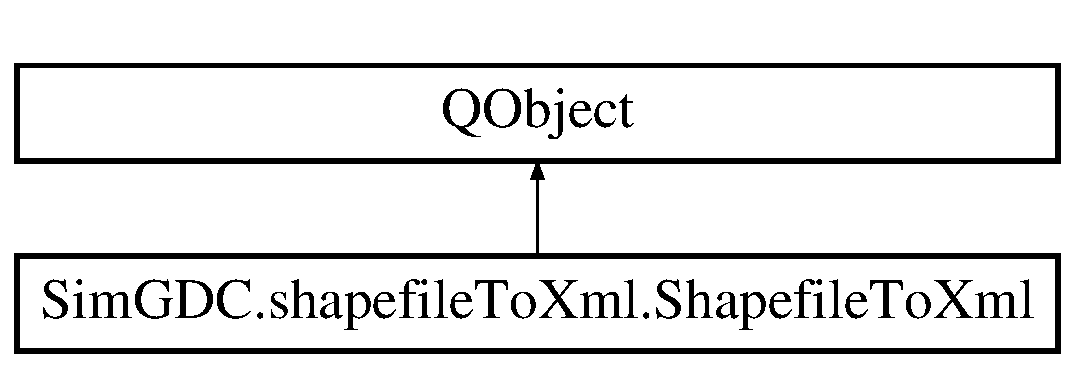
\includegraphics[height=2.000000cm]{class_sim_g_d_c_1_1shapefile_to_xml_1_1_shapefile_to_xml}
\end{center}
\end{figure}
\subsection*{Public Member Functions}
\begin{DoxyCompactItemize}
\item 
\hypertarget{class_sim_g_d_c_1_1shapefile_to_xml_1_1_shapefile_to_xml_aff17ac55db99b75946707f7e9da93636}{}def {\bfseries \+\_\+\+\_\+init\+\_\+\+\_\+} (self, xml\+Path, sh\+Dir, formula)\label{class_sim_g_d_c_1_1shapefile_to_xml_1_1_shapefile_to_xml_aff17ac55db99b75946707f7e9da93636}

\item 
\hypertarget{class_sim_g_d_c_1_1shapefile_to_xml_1_1_shapefile_to_xml_a0b9a14c672387e468405a6c9febea2ee}{}def {\bfseries warn\+Non\+Exist} (self, type\+Id, id)\label{class_sim_g_d_c_1_1shapefile_to_xml_1_1_shapefile_to_xml_a0b9a14c672387e468405a6c9febea2ee}

\item 
\hypertarget{class_sim_g_d_c_1_1shapefile_to_xml_1_1_shapefile_to_xml_ae5514d38fc6cfa6708a9498433b8ea4a}{}def {\bfseries update\+Location} (self, element, data)\label{class_sim_g_d_c_1_1shapefile_to_xml_1_1_shapefile_to_xml_ae5514d38fc6cfa6708a9498433b8ea4a}

\item 
\hypertarget{class_sim_g_d_c_1_1shapefile_to_xml_1_1_shapefile_to_xml_a5043425c38dcf6683929ca04853a9ec2}{}def {\bfseries add\+X\+M\+L\+Location} (self, parent, data)\label{class_sim_g_d_c_1_1shapefile_to_xml_1_1_shapefile_to_xml_a5043425c38dcf6683929ca04853a9ec2}

\item 
\hypertarget{class_sim_g_d_c_1_1shapefile_to_xml_1_1_shapefile_to_xml_a8680d10e1b3766282ec13c145cc9a306}{}def {\bfseries update\+Nodes} (self, nodes)\label{class_sim_g_d_c_1_1shapefile_to_xml_1_1_shapefile_to_xml_a8680d10e1b3766282ec13c145cc9a306}

\item 
\hypertarget{class_sim_g_d_c_1_1shapefile_to_xml_1_1_shapefile_to_xml_a14eb51fb242aa56fa422d909bedcaf65}{}def {\bfseries update\+Lane} (self, segment\+Id, lane)\label{class_sim_g_d_c_1_1shapefile_to_xml_1_1_shapefile_to_xml_a14eb51fb242aa56fa422d909bedcaf65}

\item 
\hypertarget{class_sim_g_d_c_1_1shapefile_to_xml_1_1_shapefile_to_xml_a4f9c4e3386576c42f4f2fac59f7b3ff2}{}def {\bfseries update\+Lane\+Edge} (self, segment\+Id, lane\+Edge)\label{class_sim_g_d_c_1_1shapefile_to_xml_1_1_shapefile_to_xml_a4f9c4e3386576c42f4f2fac59f7b3ff2}

\item 
\hypertarget{class_sim_g_d_c_1_1shapefile_to_xml_1_1_shapefile_to_xml_a1ff7dfebfc35994708b84d4e372c1ff5}{}def {\bfseries update\+Crossing} (self, segment\+Id, crossing)\label{class_sim_g_d_c_1_1shapefile_to_xml_1_1_shapefile_to_xml_a1ff7dfebfc35994708b84d4e372c1ff5}

\item 
\hypertarget{class_sim_g_d_c_1_1shapefile_to_xml_1_1_shapefile_to_xml_a739c38d00f5629df50539ec6ce30a005}{}def {\bfseries update\+Busstop} (self, segment\+Id, busstop)\label{class_sim_g_d_c_1_1shapefile_to_xml_1_1_shapefile_to_xml_a739c38d00f5629df50539ec6ce30a005}

\item 
\hypertarget{class_sim_g_d_c_1_1shapefile_to_xml_1_1_shapefile_to_xml_ab1fab8721ed3da91ebcbdfa89403e64e}{}def {\bfseries update\+Segment} (self, link\+Id, segment)\label{class_sim_g_d_c_1_1shapefile_to_xml_1_1_shapefile_to_xml_ab1fab8721ed3da91ebcbdfa89403e64e}

\item 
\hypertarget{class_sim_g_d_c_1_1shapefile_to_xml_1_1_shapefile_to_xml_a8fbd657c5099e01d1237db4653764e2b}{}def {\bfseries write\+Pretty\+To\+Xml} (self)\label{class_sim_g_d_c_1_1shapefile_to_xml_1_1_shapefile_to_xml_a8fbd657c5099e01d1237db4653764e2b}

\item 
\hypertarget{class_sim_g_d_c_1_1shapefile_to_xml_1_1_shapefile_to_xml_a3dc80764feac235beb6981740fbd0374}{}def {\bfseries run} (self)\label{class_sim_g_d_c_1_1shapefile_to_xml_1_1_shapefile_to_xml_a3dc80764feac235beb6981740fbd0374}

\end{DoxyCompactItemize}
\subsection*{Public Attributes}
\begin{DoxyCompactItemize}
\item 
\hypertarget{class_sim_g_d_c_1_1shapefile_to_xml_1_1_shapefile_to_xml_ad0719b934250ab35f1b2dcf427fab65b}{}{\bfseries xml\+Path}\label{class_sim_g_d_c_1_1shapefile_to_xml_1_1_shapefile_to_xml_ad0719b934250ab35f1b2dcf427fab65b}

\item 
\hypertarget{class_sim_g_d_c_1_1shapefile_to_xml_1_1_shapefile_to_xml_a1a1ca1adf1b003c19cb4a725a6d8e66a}{}{\bfseries reader}\label{class_sim_g_d_c_1_1shapefile_to_xml_1_1_shapefile_to_xml_a1a1ca1adf1b003c19cb4a725a6d8e66a}

\item 
\hypertarget{class_sim_g_d_c_1_1shapefile_to_xml_1_1_shapefile_to_xml_a346d3edc3fe454025508e3e39a7b0ad1}{}{\bfseries document}\label{class_sim_g_d_c_1_1shapefile_to_xml_1_1_shapefile_to_xml_a346d3edc3fe454025508e3e39a7b0ad1}

\item 
\hypertarget{class_sim_g_d_c_1_1shapefile_to_xml_1_1_shapefile_to_xml_a2871a5d7adbcb85b1d6153f3c0ade90f}{}{\bfseries formula}\label{class_sim_g_d_c_1_1shapefile_to_xml_1_1_shapefile_to_xml_a2871a5d7adbcb85b1d6153f3c0ade90f}

\end{DoxyCompactItemize}
\subsection*{Static Public Attributes}
\begin{DoxyCompactItemize}
\item 
\hypertarget{class_sim_g_d_c_1_1shapefile_to_xml_1_1_shapefile_to_xml_a2ad74bf7d4a169253b742a1d0da07f7c}{}tuple {\bfseries prog\+\_\+sig} = pyqt\+Signal(int)\label{class_sim_g_d_c_1_1shapefile_to_xml_1_1_shapefile_to_xml_a2ad74bf7d4a169253b742a1d0da07f7c}

\end{DoxyCompactItemize}


The documentation for this class was generated from the following file\+:\begin{DoxyCompactItemize}
\item 
shapefile\+To\+Xml.\+py\end{DoxyCompactItemize}

\hypertarget{class_sim_g_d_c_1_1shapefile_i_o_1_1_shapefile_writer}{}\section{Sim\+G\+D\+C.\+shapefile\+I\+O.\+Shapefile\+Writer Class Reference}
\label{class_sim_g_d_c_1_1shapefile_i_o_1_1_shapefile_writer}\index{Sim\+G\+D\+C.\+shapefile\+I\+O.\+Shapefile\+Writer@{Sim\+G\+D\+C.\+shapefile\+I\+O.\+Shapefile\+Writer}}
\subsection*{Public Member Functions}
\begin{DoxyCompactItemize}
\item 
\hypertarget{class_sim_g_d_c_1_1shapefile_i_o_1_1_shapefile_writer_a3103186744e4bff48bb15d2ee646b0dd}{}def {\bfseries \+\_\+\+\_\+init\+\_\+\+\_\+} (self, path)\label{class_sim_g_d_c_1_1shapefile_i_o_1_1_shapefile_writer_a3103186744e4bff48bb15d2ee646b0dd}

\item 
\hypertarget{class_sim_g_d_c_1_1shapefile_i_o_1_1_shapefile_writer_a9d2de70bd7f040ce2c7e86a0f156e3f7}{}def {\bfseries add\+Point} (self, typeid, point, attr)\label{class_sim_g_d_c_1_1shapefile_i_o_1_1_shapefile_writer_a9d2de70bd7f040ce2c7e86a0f156e3f7}

\item 
\hypertarget{class_sim_g_d_c_1_1shapefile_i_o_1_1_shapefile_writer_addc5d74c757899a857d40ca9586632f1}{}def {\bfseries add\+Polygon} (self, typeid, coordinates, attr)\label{class_sim_g_d_c_1_1shapefile_i_o_1_1_shapefile_writer_addc5d74c757899a857d40ca9586632f1}

\item 
\hypertarget{class_sim_g_d_c_1_1shapefile_i_o_1_1_shapefile_writer_a1f7d00798043e1f3eebeb7f0818798d3}{}def {\bfseries add\+Polyline} (self, typeid, coordinates, attr)\label{class_sim_g_d_c_1_1shapefile_i_o_1_1_shapefile_writer_a1f7d00798043e1f3eebeb7f0818798d3}

\item 
\hypertarget{class_sim_g_d_c_1_1shapefile_i_o_1_1_shapefile_writer_a5ffba693310b978849b3a575b473982d}{}def {\bfseries save} (self)\label{class_sim_g_d_c_1_1shapefile_i_o_1_1_shapefile_writer_a5ffba693310b978849b3a575b473982d}

\end{DoxyCompactItemize}
\subsection*{Public Attributes}
\begin{DoxyCompactItemize}
\item 
\hypertarget{class_sim_g_d_c_1_1shapefile_i_o_1_1_shapefile_writer_abc6abdc5df2337cf780c89b321147f0b}{}{\bfseries path}\label{class_sim_g_d_c_1_1shapefile_i_o_1_1_shapefile_writer_abc6abdc5df2337cf780c89b321147f0b}

\item 
\hypertarget{class_sim_g_d_c_1_1shapefile_i_o_1_1_shapefile_writer_a69867510e31dc606dc77ce7625711ed1}{}{\bfseries prefix}\label{class_sim_g_d_c_1_1shapefile_i_o_1_1_shapefile_writer_a69867510e31dc606dc77ce7625711ed1}

\item 
\hypertarget{class_sim_g_d_c_1_1shapefile_i_o_1_1_shapefile_writer_ab159e320c98d6f9ff46e280a24472743}{}{\bfseries layer}\label{class_sim_g_d_c_1_1shapefile_i_o_1_1_shapefile_writer_ab159e320c98d6f9ff46e280a24472743}

\end{DoxyCompactItemize}


The documentation for this class was generated from the following file\+:\begin{DoxyCompactItemize}
\item 
shapefile\+I\+O.\+py\end{DoxyCompactItemize}

\hypertarget{class_sim_g_d_c_1_1simgdc_1_1_sim_g_d_c}{}\section{Sim\+G\+D\+C.\+simgdc.\+Sim\+G\+D\+C Class Reference}
\label{class_sim_g_d_c_1_1simgdc_1_1_sim_g_d_c}\index{Sim\+G\+D\+C.\+simgdc.\+Sim\+G\+D\+C@{Sim\+G\+D\+C.\+simgdc.\+Sim\+G\+D\+C}}
\subsection*{Public Member Functions}
\begin{DoxyCompactItemize}
\item 
\hypertarget{class_sim_g_d_c_1_1simgdc_1_1_sim_g_d_c_afc904b0a199af81e0147b00f307d9521}{}def {\bfseries \+\_\+\+\_\+init\+\_\+\+\_\+} (self, iface)\label{class_sim_g_d_c_1_1simgdc_1_1_sim_g_d_c_afc904b0a199af81e0147b00f307d9521}

\item 
\hypertarget{class_sim_g_d_c_1_1simgdc_1_1_sim_g_d_c_a33b3f0c85a7977ba4c3e9625f9d30946}{}def {\bfseries init\+Gui} (self)\label{class_sim_g_d_c_1_1simgdc_1_1_sim_g_d_c_a33b3f0c85a7977ba4c3e9625f9d30946}

\item 
\hypertarget{class_sim_g_d_c_1_1simgdc_1_1_sim_g_d_c_a156fff63f5a76883a38cf0eff0d41b60}{}def {\bfseries unload} (self)\label{class_sim_g_d_c_1_1simgdc_1_1_sim_g_d_c_a156fff63f5a76883a38cf0eff0d41b60}

\item 
\hypertarget{class_sim_g_d_c_1_1simgdc_1_1_sim_g_d_c_a0e076615a58eedaec58e363eab08447d}{}def {\bfseries new} (self)\label{class_sim_g_d_c_1_1simgdc_1_1_sim_g_d_c_a0e076615a58eedaec58e363eab08447d}

\item 
\hypertarget{class_sim_g_d_c_1_1simgdc_1_1_sim_g_d_c_a5a91eab6a89599e7e4ad37e337f596bb}{}def {\bfseries open} (self, sh\+\_\+dir)\label{class_sim_g_d_c_1_1simgdc_1_1_sim_g_d_c_a5a91eab6a89599e7e4ad37e337f596bb}

\item 
\hypertarget{class_sim_g_d_c_1_1simgdc_1_1_sim_g_d_c_a9f320f19f2557a1fcfc8bc4f8ace3e93}{}def {\bfseries converter} (self)\label{class_sim_g_d_c_1_1simgdc_1_1_sim_g_d_c_a9f320f19f2557a1fcfc8bc4f8ace3e93}

\item 
\hypertarget{class_sim_g_d_c_1_1simgdc_1_1_sim_g_d_c_a06a26c9e46c062bf2de9d64d6c4092cf}{}def {\bfseries check\+Active\+Layer\+Info} (self)\label{class_sim_g_d_c_1_1simgdc_1_1_sim_g_d_c_a06a26c9e46c062bf2de9d64d6c4092cf}

\item 
\hypertarget{class_sim_g_d_c_1_1simgdc_1_1_sim_g_d_c_a068bad88721c3b8267e3d0de77222067}{}def {\bfseries add\+Feature\+Pre} (self)\label{class_sim_g_d_c_1_1simgdc_1_1_sim_g_d_c_a068bad88721c3b8267e3d0de77222067}

\item 
\hypertarget{class_sim_g_d_c_1_1simgdc_1_1_sim_g_d_c_a941a289f08149df483252841015c7e0f}{}def {\bfseries add\+Feature} (self, point, button)\label{class_sim_g_d_c_1_1simgdc_1_1_sim_g_d_c_a941a289f08149df483252841015c7e0f}

\item 
\hypertarget{class_sim_g_d_c_1_1simgdc_1_1_sim_g_d_c_a066f2cbfad352fe719dabc39da7047f0}{}def {\bfseries edit\+Feature} (self)\label{class_sim_g_d_c_1_1simgdc_1_1_sim_g_d_c_a066f2cbfad352fe719dabc39da7047f0}

\item 
\hypertarget{class_sim_g_d_c_1_1simgdc_1_1_sim_g_d_c_aa97fcbea616c254ddc8a7705effd5f07}{}def {\bfseries delete\+Feature} (self)\label{class_sim_g_d_c_1_1simgdc_1_1_sim_g_d_c_aa97fcbea616c254ddc8a7705effd5f07}

\item 
\hypertarget{class_sim_g_d_c_1_1simgdc_1_1_sim_g_d_c_ab69e458bd15161c3eaa9928c7fe09bfc}{}def {\bfseries manage\+Links} (self)\label{class_sim_g_d_c_1_1simgdc_1_1_sim_g_d_c_ab69e458bd15161c3eaa9928c7fe09bfc}

\item 
\hypertarget{class_sim_g_d_c_1_1simgdc_1_1_sim_g_d_c_ae83ba7f0c9cfb525b785260137b0ef06}{}def {\bfseries generate\+Lane} (self)\label{class_sim_g_d_c_1_1simgdc_1_1_sim_g_d_c_ae83ba7f0c9cfb525b785260137b0ef06}

\end{DoxyCompactItemize}
\subsection*{Public Attributes}
\begin{DoxyCompactItemize}
\item 
\hypertarget{class_sim_g_d_c_1_1simgdc_1_1_sim_g_d_c_a36741877c6b2974f7c00ee682f761dd9}{}{\bfseries iface}\label{class_sim_g_d_c_1_1simgdc_1_1_sim_g_d_c_a36741877c6b2974f7c00ee682f761dd9}

\item 
\hypertarget{class_sim_g_d_c_1_1simgdc_1_1_sim_g_d_c_a186fca97fdb31870d5bd822111b2ed46}{}{\bfseries canvas}\label{class_sim_g_d_c_1_1simgdc_1_1_sim_g_d_c_a186fca97fdb31870d5bd822111b2ed46}

\item 
\hypertarget{class_sim_g_d_c_1_1simgdc_1_1_sim_g_d_c_aceecf70c77febf71f200f82e1eb91378}{}{\bfseries click\+Tool}\label{class_sim_g_d_c_1_1simgdc_1_1_sim_g_d_c_aceecf70c77febf71f200f82e1eb91378}

\item 
\hypertarget{class_sim_g_d_c_1_1simgdc_1_1_sim_g_d_c_a965a6adc3631d0e0f8c4d6a9e841ad44}{}{\bfseries tool\+Pan}\label{class_sim_g_d_c_1_1simgdc_1_1_sim_g_d_c_a965a6adc3631d0e0f8c4d6a9e841ad44}

\item 
\hypertarget{class_sim_g_d_c_1_1simgdc_1_1_sim_g_d_c_a5ee08f9b1acd4792a9029da654d341b7}{}{\bfseries converterdlg}\label{class_sim_g_d_c_1_1simgdc_1_1_sim_g_d_c_a5ee08f9b1acd4792a9029da654d341b7}

\item 
\hypertarget{class_sim_g_d_c_1_1simgdc_1_1_sim_g_d_c_a53aac4a63bea263f003833ef018b4649}{}{\bfseries featuredlg}\label{class_sim_g_d_c_1_1simgdc_1_1_sim_g_d_c_a53aac4a63bea263f003833ef018b4649}

\item 
\hypertarget{class_sim_g_d_c_1_1simgdc_1_1_sim_g_d_c_ac1d728cb319a1fa9c8d505ddb0fcc0e5}{}{\bfseries plugin\+\_\+dir}\label{class_sim_g_d_c_1_1simgdc_1_1_sim_g_d_c_ac1d728cb319a1fa9c8d505ddb0fcc0e5}

\item 
\hypertarget{class_sim_g_d_c_1_1simgdc_1_1_sim_g_d_c_a2df7c6e9d99ef5c86beb656f5c08a1a9}{}{\bfseries translator}\label{class_sim_g_d_c_1_1simgdc_1_1_sim_g_d_c_a2df7c6e9d99ef5c86beb656f5c08a1a9}

\item 
\hypertarget{class_sim_g_d_c_1_1simgdc_1_1_sim_g_d_c_acf09c8e29f6034401b8c08a4077ddd1b}{}{\bfseries converter\+\_\+action}\label{class_sim_g_d_c_1_1simgdc_1_1_sim_g_d_c_acf09c8e29f6034401b8c08a4077ddd1b}

\item 
\hypertarget{class_sim_g_d_c_1_1simgdc_1_1_sim_g_d_c_a5373c408da7d6032b6fb34862c717a7e}{}{\bfseries open\+\_\+action}\label{class_sim_g_d_c_1_1simgdc_1_1_sim_g_d_c_a5373c408da7d6032b6fb34862c717a7e}

\item 
\hypertarget{class_sim_g_d_c_1_1simgdc_1_1_sim_g_d_c_af41cb607ef8832224eaf61a520d64206}{}{\bfseries new\+\_\+action}\label{class_sim_g_d_c_1_1simgdc_1_1_sim_g_d_c_af41cb607ef8832224eaf61a520d64206}

\item 
\hypertarget{class_sim_g_d_c_1_1simgdc_1_1_sim_g_d_c_a38e5cc7f00b8e270daf1211820c993bc}{}{\bfseries link\+\_\+manager\+\_\+action}\label{class_sim_g_d_c_1_1simgdc_1_1_sim_g_d_c_a38e5cc7f00b8e270daf1211820c993bc}

\item 
\hypertarget{class_sim_g_d_c_1_1simgdc_1_1_sim_g_d_c_adad5b1a03b9997e09532c4a4f6c08409}{}{\bfseries add\+\_\+action}\label{class_sim_g_d_c_1_1simgdc_1_1_sim_g_d_c_adad5b1a03b9997e09532c4a4f6c08409}

\item 
\hypertarget{class_sim_g_d_c_1_1simgdc_1_1_sim_g_d_c_a926fe6f8cd21557369c6a178c604a47f}{}{\bfseries edit\+\_\+action}\label{class_sim_g_d_c_1_1simgdc_1_1_sim_g_d_c_a926fe6f8cd21557369c6a178c604a47f}

\item 
\hypertarget{class_sim_g_d_c_1_1simgdc_1_1_sim_g_d_c_ac6b8868f7287a705fa3a55345b52e5e9}{}{\bfseries delete\+\_\+action}\label{class_sim_g_d_c_1_1simgdc_1_1_sim_g_d_c_ac6b8868f7287a705fa3a55345b52e5e9}

\item 
\hypertarget{class_sim_g_d_c_1_1simgdc_1_1_sim_g_d_c_a0a5b2b92bd1d430e0905818ce60817a5}{}{\bfseries gen\+\_\+lane\+\_\+action}\label{class_sim_g_d_c_1_1simgdc_1_1_sim_g_d_c_a0a5b2b92bd1d430e0905818ce60817a5}

\end{DoxyCompactItemize}


The documentation for this class was generated from the following file\+:\begin{DoxyCompactItemize}
\item 
simgdc.\+py\end{DoxyCompactItemize}

\hypertarget{class_sim_g_d_c_1_1trainstop__dialog_1_1_trainstop_dialog}{}\section{Sim\+G\+D\+C.\+trainstop\+\_\+dialog.\+Trainstop\+Dialog Class Reference}
\label{class_sim_g_d_c_1_1trainstop__dialog_1_1_trainstop_dialog}\index{Sim\+G\+D\+C.\+trainstop\+\_\+dialog.\+Trainstop\+Dialog@{Sim\+G\+D\+C.\+trainstop\+\_\+dialog.\+Trainstop\+Dialog}}
Inheritance diagram for Sim\+G\+D\+C.\+trainstop\+\_\+dialog.\+Trainstop\+Dialog\+:\begin{figure}[H]
\begin{center}
\leavevmode
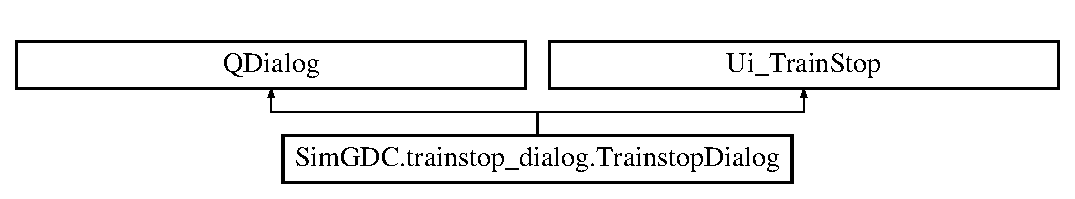
\includegraphics[height=2.000000cm]{class_sim_g_d_c_1_1trainstop__dialog_1_1_trainstop_dialog}
\end{center}
\end{figure}
\subsection*{Public Member Functions}
\begin{DoxyCompactItemize}
\item 
\hypertarget{class_sim_g_d_c_1_1trainstop__dialog_1_1_trainstop_dialog_a37d4b013742910df9ea86d47b65f5faa}{}def {\bfseries \+\_\+\+\_\+init\+\_\+\+\_\+} (self)\label{class_sim_g_d_c_1_1trainstop__dialog_1_1_trainstop_dialog_a37d4b013742910df9ea86d47b65f5faa}

\item 
\hypertarget{class_sim_g_d_c_1_1trainstop__dialog_1_1_trainstop_dialog_a75a9527177e4662ed7c21b4a47a43ce4}{}def {\bfseries get\+Segment\+List} (self)\label{class_sim_g_d_c_1_1trainstop__dialog_1_1_trainstop_dialog_a75a9527177e4662ed7c21b4a47a43ce4}

\item 
\hypertarget{class_sim_g_d_c_1_1trainstop__dialog_1_1_trainstop_dialog_acc2eaa80b66993a3facf0157fd7f4ea0}{}def {\bfseries set\+Segment\+List} (self)\label{class_sim_g_d_c_1_1trainstop__dialog_1_1_trainstop_dialog_acc2eaa80b66993a3facf0157fd7f4ea0}

\item 
\hypertarget{class_sim_g_d_c_1_1trainstop__dialog_1_1_trainstop_dialog_a5f2848bbf5be7973dbdbce733c343f7a}{}def {\bfseries add\+Segment} (self)\label{class_sim_g_d_c_1_1trainstop__dialog_1_1_trainstop_dialog_a5f2848bbf5be7973dbdbce733c343f7a}

\item 
\hypertarget{class_sim_g_d_c_1_1trainstop__dialog_1_1_trainstop_dialog_a99d14faa65e6d8d609152a0be3ce394f}{}def {\bfseries addnewid} (self)\label{class_sim_g_d_c_1_1trainstop__dialog_1_1_trainstop_dialog_a99d14faa65e6d8d609152a0be3ce394f}

\item 
\hypertarget{class_sim_g_d_c_1_1trainstop__dialog_1_1_trainstop_dialog_aaa6cad34279e870e3781336e86bcbf4b}{}def {\bfseries set\+Segment\+Id} (self, seg\+I\+Dstring)\label{class_sim_g_d_c_1_1trainstop__dialog_1_1_trainstop_dialog_aaa6cad34279e870e3781336e86bcbf4b}

\item 
\hypertarget{class_sim_g_d_c_1_1trainstop__dialog_1_1_trainstop_dialog_a339ca5b430b72c86c15bc2954fe81e63}{}def {\bfseries set\+Info} (self, info)\label{class_sim_g_d_c_1_1trainstop__dialog_1_1_trainstop_dialog_a339ca5b430b72c86c15bc2954fe81e63}

\item 
\hypertarget{class_sim_g_d_c_1_1trainstop__dialog_1_1_trainstop_dialog_a2b36dd8881b6f8d07517038a81e77a63}{}def {\bfseries update} (self)\label{class_sim_g_d_c_1_1trainstop__dialog_1_1_trainstop_dialog_a2b36dd8881b6f8d07517038a81e77a63}

\end{DoxyCompactItemize}
\subsection*{Public Attributes}
\begin{DoxyCompactItemize}
\item 
\hypertarget{class_sim_g_d_c_1_1trainstop__dialog_1_1_trainstop_dialog_a07e00a6e48a129de26805aad8484340d}{}{\bfseries info}\label{class_sim_g_d_c_1_1trainstop__dialog_1_1_trainstop_dialog_a07e00a6e48a129de26805aad8484340d}

\item 
\hypertarget{class_sim_g_d_c_1_1trainstop__dialog_1_1_trainstop_dialog_af28f009f771126aaafeec5509aea4907}{}{\bfseries is\+Modified}\label{class_sim_g_d_c_1_1trainstop__dialog_1_1_trainstop_dialog_af28f009f771126aaafeec5509aea4907}

\end{DoxyCompactItemize}
\subsection*{Static Public Attributes}
\begin{DoxyCompactItemize}
\item 
\hypertarget{class_sim_g_d_c_1_1trainstop__dialog_1_1_trainstop_dialog_ae785f8eabc0358089a1c14a64771b455}{}int {\bfseries original\+\_\+id} = 0\label{class_sim_g_d_c_1_1trainstop__dialog_1_1_trainstop_dialog_ae785f8eabc0358089a1c14a64771b455}

\end{DoxyCompactItemize}


The documentation for this class was generated from the following file\+:\begin{DoxyCompactItemize}
\item 
trainstop\+\_\+dialog.\+py\end{DoxyCompactItemize}

\hypertarget{class_sim_g_d_c_1_1ui__busstop_1_1_ui___busstop}{}\section{Sim\+G\+D\+C.\+ui\+\_\+busstop.\+Ui\+\_\+\+Busstop Class Reference}
\label{class_sim_g_d_c_1_1ui__busstop_1_1_ui___busstop}\index{Sim\+G\+D\+C.\+ui\+\_\+busstop.\+Ui\+\_\+\+Busstop@{Sim\+G\+D\+C.\+ui\+\_\+busstop.\+Ui\+\_\+\+Busstop}}
Inheritance diagram for Sim\+G\+D\+C.\+ui\+\_\+busstop.\+Ui\+\_\+\+Busstop\+:\begin{figure}[H]
\begin{center}
\leavevmode
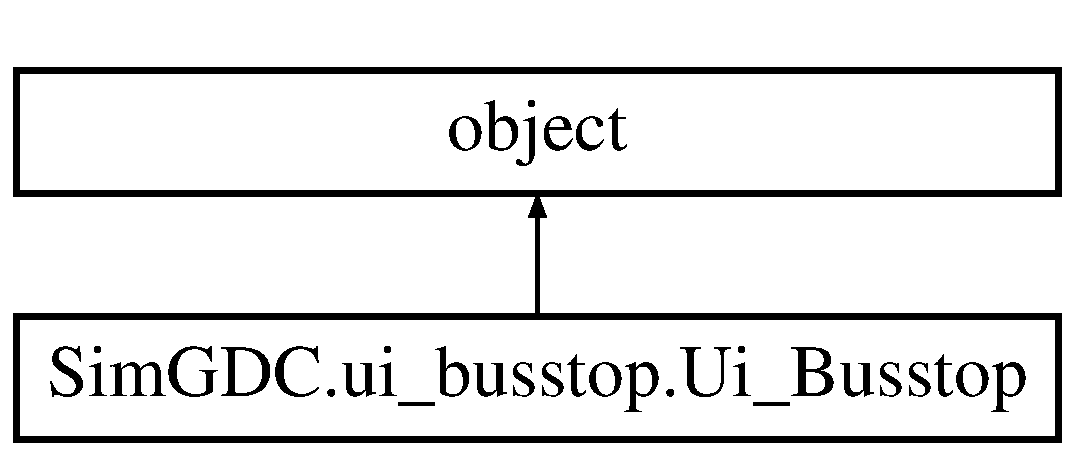
\includegraphics[height=2.000000cm]{class_sim_g_d_c_1_1ui__busstop_1_1_ui___busstop}
\end{center}
\end{figure}
\subsection*{Public Member Functions}
\begin{DoxyCompactItemize}
\item 
\hypertarget{class_sim_g_d_c_1_1ui__busstop_1_1_ui___busstop_a495a602fa4551985777656dd495d6498}{}def {\bfseries setup\+Ui} (self, Busstop)\label{class_sim_g_d_c_1_1ui__busstop_1_1_ui___busstop_a495a602fa4551985777656dd495d6498}

\item 
\hypertarget{class_sim_g_d_c_1_1ui__busstop_1_1_ui___busstop_ace330819588006f630f266b90ae270b5}{}def {\bfseries retranslate\+Ui} (self, Busstop)\label{class_sim_g_d_c_1_1ui__busstop_1_1_ui___busstop_ace330819588006f630f266b90ae270b5}

\end{DoxyCompactItemize}
\subsection*{Public Attributes}
\begin{DoxyCompactItemize}
\item 
\hypertarget{class_sim_g_d_c_1_1ui__busstop_1_1_ui___busstop_a682ceab01c25f133ad2156a9dd019a83}{}{\bfseries Segment\+Group\+Box}\label{class_sim_g_d_c_1_1ui__busstop_1_1_ui___busstop_a682ceab01c25f133ad2156a9dd019a83}

\item 
\hypertarget{class_sim_g_d_c_1_1ui__busstop_1_1_ui___busstop_aba0327157a8b32cd9781f39e2cbfbdb8}{}{\bfseries segment\+Idlabel}\label{class_sim_g_d_c_1_1ui__busstop_1_1_ui___busstop_aba0327157a8b32cd9781f39e2cbfbdb8}

\item 
\hypertarget{class_sim_g_d_c_1_1ui__busstop_1_1_ui___busstop_a95bc1e62f7a5b23819a7b6653c7e289a}{}{\bfseries segment\+I\+Dcombo\+Box}\label{class_sim_g_d_c_1_1ui__busstop_1_1_ui___busstop_a95bc1e62f7a5b23819a7b6653c7e289a}

\item 
\hypertarget{class_sim_g_d_c_1_1ui__busstop_1_1_ui___busstop_a3ce38c654a8786baad167dddca7826b9}{}{\bfseries title\+Label}\label{class_sim_g_d_c_1_1ui__busstop_1_1_ui___busstop_a3ce38c654a8786baad167dddca7826b9}

\item 
\hypertarget{class_sim_g_d_c_1_1ui__busstop_1_1_ui___busstop_a033013e018f4f77f0d1e20c07600b2d0}{}{\bfseries attribute\+Group}\label{class_sim_g_d_c_1_1ui__busstop_1_1_ui___busstop_a033013e018f4f77f0d1e20c07600b2d0}

\item 
\hypertarget{class_sim_g_d_c_1_1ui__busstop_1_1_ui___busstop_ae1cc611d57efe288f21b2e55fac01ddb}{}{\bfseries has\+Shelter}\label{class_sim_g_d_c_1_1ui__busstop_1_1_ui___busstop_ae1cc611d57efe288f21b2e55fac01ddb}

\item 
\hypertarget{class_sim_g_d_c_1_1ui__busstop_1_1_ui___busstop_a7c93c5cfad62f9375a17eccedbe0d984}{}{\bfseries label\+\_\+2}\label{class_sim_g_d_c_1_1ui__busstop_1_1_ui___busstop_a7c93c5cfad62f9375a17eccedbe0d984}

\item 
\hypertarget{class_sim_g_d_c_1_1ui__busstop_1_1_ui___busstop_a3d70cec3591e3aecbb3f52e4f038d240}{}{\bfseries label\+\_\+3}\label{class_sim_g_d_c_1_1ui__busstop_1_1_ui___busstop_a3d70cec3591e3aecbb3f52e4f038d240}

\item 
\hypertarget{class_sim_g_d_c_1_1ui__busstop_1_1_ui___busstop_a805bd8a36943d866037af5e1676b77b5}{}{\bfseries length}\label{class_sim_g_d_c_1_1ui__busstop_1_1_ui___busstop_a805bd8a36943d866037af5e1676b77b5}

\item 
\hypertarget{class_sim_g_d_c_1_1ui__busstop_1_1_ui___busstop_a8e005264b2c44b3448fcd4721974af31}{}{\bfseries busstoptags}\label{class_sim_g_d_c_1_1ui__busstop_1_1_ui___busstop_a8e005264b2c44b3448fcd4721974af31}

\item 
\hypertarget{class_sim_g_d_c_1_1ui__busstop_1_1_ui___busstop_a422fa7bd8db54d3ca8138bcace5cf704}{}{\bfseries is\+Terminal}\label{class_sim_g_d_c_1_1ui__busstop_1_1_ui___busstop_a422fa7bd8db54d3ca8138bcace5cf704}

\item 
\hypertarget{class_sim_g_d_c_1_1ui__busstop_1_1_ui___busstop_ad53b4c13b90625a2b164e8852ad4a6d7}{}{\bfseries is\+Bay}\label{class_sim_g_d_c_1_1ui__busstop_1_1_ui___busstop_ad53b4c13b90625a2b164e8852ad4a6d7}

\item 
\hypertarget{class_sim_g_d_c_1_1ui__busstop_1_1_ui___busstop_a16f00b0991d1911f0df9f14c5cd7601a}{}{\bfseries action\+Button}\label{class_sim_g_d_c_1_1ui__busstop_1_1_ui___busstop_a16f00b0991d1911f0df9f14c5cd7601a}

\item 
\hypertarget{class_sim_g_d_c_1_1ui__busstop_1_1_ui___busstop_ae930dc2c8a60b2b2b93a2e7022e1a5f8}{}{\bfseries id\+Label}\label{class_sim_g_d_c_1_1ui__busstop_1_1_ui___busstop_ae930dc2c8a60b2b2b93a2e7022e1a5f8}

\item 
\hypertarget{class_sim_g_d_c_1_1ui__busstop_1_1_ui___busstop_a3f21131f9bab6fe17ea8bd7ad2df9f35}{}{\bfseries id}\label{class_sim_g_d_c_1_1ui__busstop_1_1_ui___busstop_a3f21131f9bab6fe17ea8bd7ad2df9f35}

\item 
\hypertarget{class_sim_g_d_c_1_1ui__busstop_1_1_ui___busstop_a8784f71e9bc56f6c37b08fd2e6f6db2b}{}{\bfseries Offset\+Label}\label{class_sim_g_d_c_1_1ui__busstop_1_1_ui___busstop_a8784f71e9bc56f6c37b08fd2e6f6db2b}

\item 
\hypertarget{class_sim_g_d_c_1_1ui__busstop_1_1_ui___busstop_adaa3142386aa05b00e2490eab0883d9d}{}{\bfseries offset}\label{class_sim_g_d_c_1_1ui__busstop_1_1_ui___busstop_adaa3142386aa05b00e2490eab0883d9d}

\item 
\hypertarget{class_sim_g_d_c_1_1ui__busstop_1_1_ui___busstop_a153b2797096928415649958b5467edc5}{}{\bfseries widget}\label{class_sim_g_d_c_1_1ui__busstop_1_1_ui___busstop_a153b2797096928415649958b5467edc5}

\item 
\hypertarget{class_sim_g_d_c_1_1ui__busstop_1_1_ui___busstop_a5c7713e2b2801cdbe0d914c91f7806cd}{}{\bfseries horizontal\+Layout\+\_\+2}\label{class_sim_g_d_c_1_1ui__busstop_1_1_ui___busstop_a5c7713e2b2801cdbe0d914c91f7806cd}

\item 
\hypertarget{class_sim_g_d_c_1_1ui__busstop_1_1_ui___busstop_a672d72a5fcda61937af7fb38f4dff17e}{}{\bfseries bus\+Capacity\+Label}\label{class_sim_g_d_c_1_1ui__busstop_1_1_ui___busstop_a672d72a5fcda61937af7fb38f4dff17e}

\item 
\hypertarget{class_sim_g_d_c_1_1ui__busstop_1_1_ui___busstop_a0b934bc79764d93bdfebf88b4b1b5711}{}{\bfseries name}\label{class_sim_g_d_c_1_1ui__busstop_1_1_ui___busstop_a0b934bc79764d93bdfebf88b4b1b5711}

\item 
\hypertarget{class_sim_g_d_c_1_1ui__busstop_1_1_ui___busstop_a303c370629828b8ce38752a6c8ef0e98}{}{\bfseries busstop\+No\+Label}\label{class_sim_g_d_c_1_1ui__busstop_1_1_ui___busstop_a303c370629828b8ce38752a6c8ef0e98}

\item 
\hypertarget{class_sim_g_d_c_1_1ui__busstop_1_1_ui___busstop_acdf311a1c8d37291b8312ddc6f9257dd}{}{\bfseries busstop\+Code}\label{class_sim_g_d_c_1_1ui__busstop_1_1_ui___busstop_acdf311a1c8d37291b8312ddc6f9257dd}

\end{DoxyCompactItemize}


The documentation for this class was generated from the following file\+:\begin{DoxyCompactItemize}
\item 
ui\+\_\+busstop.\+py\end{DoxyCompactItemize}

\hypertarget{class_sim_g_d_c_1_1ui__converter_1_1_ui___converter}{}\section{Sim\+G\+D\+C.\+ui\+\_\+converter.\+Ui\+\_\+\+Converter Class Reference}
\label{class_sim_g_d_c_1_1ui__converter_1_1_ui___converter}\index{Sim\+G\+D\+C.\+ui\+\_\+converter.\+Ui\+\_\+\+Converter@{Sim\+G\+D\+C.\+ui\+\_\+converter.\+Ui\+\_\+\+Converter}}
Inheritance diagram for Sim\+G\+D\+C.\+ui\+\_\+converter.\+Ui\+\_\+\+Converter\+:\begin{figure}[H]
\begin{center}
\leavevmode
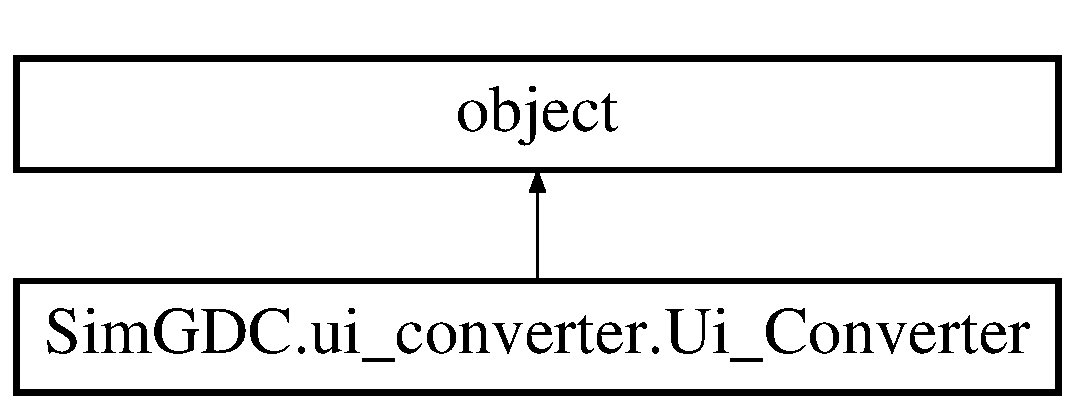
\includegraphics[height=2.000000cm]{class_sim_g_d_c_1_1ui__converter_1_1_ui___converter}
\end{center}
\end{figure}
\subsection*{Public Member Functions}
\begin{DoxyCompactItemize}
\item 
\hypertarget{class_sim_g_d_c_1_1ui__converter_1_1_ui___converter_a0a1266647491792c2b5f175f5c7c9bbe}{}def {\bfseries setup\+Ui} (self, Converter)\label{class_sim_g_d_c_1_1ui__converter_1_1_ui___converter_a0a1266647491792c2b5f175f5c7c9bbe}

\item 
\hypertarget{class_sim_g_d_c_1_1ui__converter_1_1_ui___converter_ae023a354ab1af676c91eba5bb6c32ba6}{}def {\bfseries retranslate\+Ui} (self, Converter)\label{class_sim_g_d_c_1_1ui__converter_1_1_ui___converter_ae023a354ab1af676c91eba5bb6c32ba6}

\end{DoxyCompactItemize}
\subsection*{Public Attributes}
\begin{DoxyCompactItemize}
\item 
\hypertarget{class_sim_g_d_c_1_1ui__converter_1_1_ui___converter_af623afd5a3afaea3abf6dbd94325efa3}{}{\bfseries tab\+Widget}\label{class_sim_g_d_c_1_1ui__converter_1_1_ui___converter_af623afd5a3afaea3abf6dbd94325efa3}

\item 
\hypertarget{class_sim_g_d_c_1_1ui__converter_1_1_ui___converter_acafe5d7b943b2c1d5991d28d285b9d4d}{}{\bfseries X\+M\+Lto\+S\+H}\label{class_sim_g_d_c_1_1ui__converter_1_1_ui___converter_acafe5d7b943b2c1d5991d28d285b9d4d}

\item 
\hypertarget{class_sim_g_d_c_1_1ui__converter_1_1_ui___converter_aa9a34dd1f6369bd5e8fa76324dcc0871}{}{\bfseries xmlsh\+\_\+converter\+\_\+but}\label{class_sim_g_d_c_1_1ui__converter_1_1_ui___converter_aa9a34dd1f6369bd5e8fa76324dcc0871}

\item 
\hypertarget{class_sim_g_d_c_1_1ui__converter_1_1_ui___converter_ab74b530e70d4c847b4d3622087904469}{}{\bfseries xmlsh\+\_\+progress}\label{class_sim_g_d_c_1_1ui__converter_1_1_ui___converter_ab74b530e70d4c847b4d3622087904469}

\item 
\hypertarget{class_sim_g_d_c_1_1ui__converter_1_1_ui___converter_a89045b524e74aca04449b0e4d693c992}{}{\bfseries xmlsh\+\_\+status}\label{class_sim_g_d_c_1_1ui__converter_1_1_ui___converter_a89045b524e74aca04449b0e4d693c992}

\item 
\hypertarget{class_sim_g_d_c_1_1ui__converter_1_1_ui___converter_acc474216db4bcc3222c96080b1148e27}{}{\bfseries widget}\label{class_sim_g_d_c_1_1ui__converter_1_1_ui___converter_acc474216db4bcc3222c96080b1148e27}

\item 
\hypertarget{class_sim_g_d_c_1_1ui__converter_1_1_ui___converter_a570820758b2c200c3288d4a30adc14fd}{}{\bfseries horizontal\+Layout}\label{class_sim_g_d_c_1_1ui__converter_1_1_ui___converter_a570820758b2c200c3288d4a30adc14fd}

\item 
\hypertarget{class_sim_g_d_c_1_1ui__converter_1_1_ui___converter_a9e889a7d2be2942444ccc255dbcb52e3}{}{\bfseries xmlsh\+\_\+xml\+\_\+label}\label{class_sim_g_d_c_1_1ui__converter_1_1_ui___converter_a9e889a7d2be2942444ccc255dbcb52e3}

\item 
\hypertarget{class_sim_g_d_c_1_1ui__converter_1_1_ui___converter_a0b898cd0f48c2820a48ad4fe629ad302}{}{\bfseries xmlsh\+\_\+xml\+\_\+path}\label{class_sim_g_d_c_1_1ui__converter_1_1_ui___converter_a0b898cd0f48c2820a48ad4fe629ad302}

\item 
\hypertarget{class_sim_g_d_c_1_1ui__converter_1_1_ui___converter_a1a55da24739eb40d1b245417741b1faa}{}{\bfseries xmlsh\+\_\+xml\+\_\+browser}\label{class_sim_g_d_c_1_1ui__converter_1_1_ui___converter_a1a55da24739eb40d1b245417741b1faa}

\item 
\hypertarget{class_sim_g_d_c_1_1ui__converter_1_1_ui___converter_a54a7880f100b0eb9eb084bb821fab2b9}{}{\bfseries widget1}\label{class_sim_g_d_c_1_1ui__converter_1_1_ui___converter_a54a7880f100b0eb9eb084bb821fab2b9}

\item 
\hypertarget{class_sim_g_d_c_1_1ui__converter_1_1_ui___converter_a060b1206fa7f21bc0495c3fae789da84}{}{\bfseries horizontal\+Layout\+\_\+2}\label{class_sim_g_d_c_1_1ui__converter_1_1_ui___converter_a060b1206fa7f21bc0495c3fae789da84}

\item 
\hypertarget{class_sim_g_d_c_1_1ui__converter_1_1_ui___converter_a3a99db47141b4c30f42711ee489b077c}{}{\bfseries xmlsh\+\_\+sh\+\_\+label}\label{class_sim_g_d_c_1_1ui__converter_1_1_ui___converter_a3a99db47141b4c30f42711ee489b077c}

\item 
\hypertarget{class_sim_g_d_c_1_1ui__converter_1_1_ui___converter_a4939cc8c8599b1bd3488ec21e24ec5be}{}{\bfseries xmlsh\+\_\+sh\+\_\+path}\label{class_sim_g_d_c_1_1ui__converter_1_1_ui___converter_a4939cc8c8599b1bd3488ec21e24ec5be}

\item 
\hypertarget{class_sim_g_d_c_1_1ui__converter_1_1_ui___converter_a22f51ecaeb64f733b8fa015e8214e321}{}{\bfseries xmlsh\+\_\+sh\+\_\+browser}\label{class_sim_g_d_c_1_1ui__converter_1_1_ui___converter_a22f51ecaeb64f733b8fa015e8214e321}

\item 
\hypertarget{class_sim_g_d_c_1_1ui__converter_1_1_ui___converter_a77e2e2da98f0b1dab4d685b4d37d5360}{}{\bfseries widget2}\label{class_sim_g_d_c_1_1ui__converter_1_1_ui___converter_a77e2e2da98f0b1dab4d685b4d37d5360}

\item 
\hypertarget{class_sim_g_d_c_1_1ui__converter_1_1_ui___converter_a51b67cfde8fa440fdaa63ab40eb853f9}{}{\bfseries horizontal\+Layout\+\_\+3}\label{class_sim_g_d_c_1_1ui__converter_1_1_ui___converter_a51b67cfde8fa440fdaa63ab40eb853f9}

\item 
\hypertarget{class_sim_g_d_c_1_1ui__converter_1_1_ui___converter_a286236244b0b791850e18abadd9baeee}{}{\bfseries xmlsh\+\_\+formula\+\_\+l1}\label{class_sim_g_d_c_1_1ui__converter_1_1_ui___converter_a286236244b0b791850e18abadd9baeee}

\item 
\hypertarget{class_sim_g_d_c_1_1ui__converter_1_1_ui___converter_a0314bbb6b08b787a0efd31b33606f5bc}{}{\bfseries xmlsh\+\_\+formula\+\_\+l2}\label{class_sim_g_d_c_1_1ui__converter_1_1_ui___converter_a0314bbb6b08b787a0efd31b33606f5bc}

\item 
\hypertarget{class_sim_g_d_c_1_1ui__converter_1_1_ui___converter_a04f3448b726ee34a6281e8d1a854ce3e}{}{\bfseries xmlsh\+\_\+formula\+\_\+x}\label{class_sim_g_d_c_1_1ui__converter_1_1_ui___converter_a04f3448b726ee34a6281e8d1a854ce3e}

\item 
\hypertarget{class_sim_g_d_c_1_1ui__converter_1_1_ui___converter_a6d94ea81c71a471351f3b3a9334ac3cb}{}{\bfseries xmlsh\+\_\+formula\+\_\+l3}\label{class_sim_g_d_c_1_1ui__converter_1_1_ui___converter_a6d94ea81c71a471351f3b3a9334ac3cb}

\item 
\hypertarget{class_sim_g_d_c_1_1ui__converter_1_1_ui___converter_a2607624e9ef45a2e2c6a0efaa2d495ea}{}{\bfseries xmlsh\+\_\+formula\+\_\+y}\label{class_sim_g_d_c_1_1ui__converter_1_1_ui___converter_a2607624e9ef45a2e2c6a0efaa2d495ea}

\item 
\hypertarget{class_sim_g_d_c_1_1ui__converter_1_1_ui___converter_ae144b6b213e1df1eb13601cfe192cda4}{}{\bfseries xmlsh\+\_\+formula\+\_\+l4}\label{class_sim_g_d_c_1_1ui__converter_1_1_ui___converter_ae144b6b213e1df1eb13601cfe192cda4}

\item 
\hypertarget{class_sim_g_d_c_1_1ui__converter_1_1_ui___converter_ad5c3b4b0d61a844ad53494c0b0e7d63c}{}{\bfseries S\+Hto\+X\+M\+L}\label{class_sim_g_d_c_1_1ui__converter_1_1_ui___converter_ad5c3b4b0d61a844ad53494c0b0e7d63c}

\item 
\hypertarget{class_sim_g_d_c_1_1ui__converter_1_1_ui___converter_abcac16c362b9cbb2275cecafb8f61cb3}{}{\bfseries shxml\+\_\+status}\label{class_sim_g_d_c_1_1ui__converter_1_1_ui___converter_abcac16c362b9cbb2275cecafb8f61cb3}

\item 
\hypertarget{class_sim_g_d_c_1_1ui__converter_1_1_ui___converter_af5d0cd5a683a7c2026dd594f796ae58c}{}{\bfseries shxml\+\_\+converter\+\_\+but}\label{class_sim_g_d_c_1_1ui__converter_1_1_ui___converter_af5d0cd5a683a7c2026dd594f796ae58c}

\item 
\hypertarget{class_sim_g_d_c_1_1ui__converter_1_1_ui___converter_a4bf244ed472558b45437d0bf48e24a8b}{}{\bfseries shxml\+\_\+progress}\label{class_sim_g_d_c_1_1ui__converter_1_1_ui___converter_a4bf244ed472558b45437d0bf48e24a8b}

\item 
\hypertarget{class_sim_g_d_c_1_1ui__converter_1_1_ui___converter_a7942b859a87e1cc8369901981a45ef54}{}{\bfseries widget3}\label{class_sim_g_d_c_1_1ui__converter_1_1_ui___converter_a7942b859a87e1cc8369901981a45ef54}

\item 
\hypertarget{class_sim_g_d_c_1_1ui__converter_1_1_ui___converter_a9f0de9c17385cc1f16c68cd3ecb4a20d}{}{\bfseries horizontal\+Layout\+\_\+4}\label{class_sim_g_d_c_1_1ui__converter_1_1_ui___converter_a9f0de9c17385cc1f16c68cd3ecb4a20d}

\item 
\hypertarget{class_sim_g_d_c_1_1ui__converter_1_1_ui___converter_a0729e2d05e464f8706e49e23ebf5ea6a}{}{\bfseries shxml\+\_\+sh\+\_\+label}\label{class_sim_g_d_c_1_1ui__converter_1_1_ui___converter_a0729e2d05e464f8706e49e23ebf5ea6a}

\item 
\hypertarget{class_sim_g_d_c_1_1ui__converter_1_1_ui___converter_a01c5ffb75b4801719f5da3cc355a2b09}{}{\bfseries shxml\+\_\+sh\+\_\+path}\label{class_sim_g_d_c_1_1ui__converter_1_1_ui___converter_a01c5ffb75b4801719f5da3cc355a2b09}

\item 
\hypertarget{class_sim_g_d_c_1_1ui__converter_1_1_ui___converter_ad77fc85667b93d45068352a736826f38}{}{\bfseries shxml\+\_\+sh\+\_\+browser}\label{class_sim_g_d_c_1_1ui__converter_1_1_ui___converter_ad77fc85667b93d45068352a736826f38}

\item 
\hypertarget{class_sim_g_d_c_1_1ui__converter_1_1_ui___converter_af2fff473b8df3224ea0cb50905ad5999}{}{\bfseries widget4}\label{class_sim_g_d_c_1_1ui__converter_1_1_ui___converter_af2fff473b8df3224ea0cb50905ad5999}

\item 
\hypertarget{class_sim_g_d_c_1_1ui__converter_1_1_ui___converter_af46eee4f438ea86f5d3b44c519f1b182}{}{\bfseries horizontal\+Layout\+\_\+5}\label{class_sim_g_d_c_1_1ui__converter_1_1_ui___converter_af46eee4f438ea86f5d3b44c519f1b182}

\item 
\hypertarget{class_sim_g_d_c_1_1ui__converter_1_1_ui___converter_ac008b8f11837306ebd70205795c6a654}{}{\bfseries shxml\+\_\+xml\+\_\+label}\label{class_sim_g_d_c_1_1ui__converter_1_1_ui___converter_ac008b8f11837306ebd70205795c6a654}

\item 
\hypertarget{class_sim_g_d_c_1_1ui__converter_1_1_ui___converter_aadfae6871b5934b165f58d940c14e69f}{}{\bfseries shxml\+\_\+xml\+\_\+path}\label{class_sim_g_d_c_1_1ui__converter_1_1_ui___converter_aadfae6871b5934b165f58d940c14e69f}

\item 
\hypertarget{class_sim_g_d_c_1_1ui__converter_1_1_ui___converter_afa6f8fd44f58be5c17a5c00a5e472364}{}{\bfseries shxml\+\_\+xml\+\_\+browser}\label{class_sim_g_d_c_1_1ui__converter_1_1_ui___converter_afa6f8fd44f58be5c17a5c00a5e472364}

\item 
\hypertarget{class_sim_g_d_c_1_1ui__converter_1_1_ui___converter_af187892a045cc83bf6af0030b0a02977}{}{\bfseries widget5}\label{class_sim_g_d_c_1_1ui__converter_1_1_ui___converter_af187892a045cc83bf6af0030b0a02977}

\item 
\hypertarget{class_sim_g_d_c_1_1ui__converter_1_1_ui___converter_a9d6825f312255fb5a65b979778365f53}{}{\bfseries horizontal\+Layout\+\_\+6}\label{class_sim_g_d_c_1_1ui__converter_1_1_ui___converter_a9d6825f312255fb5a65b979778365f53}

\item 
\hypertarget{class_sim_g_d_c_1_1ui__converter_1_1_ui___converter_a3bcd0bf067bfb3585c7f0ace939cc113}{}{\bfseries shxml\+\_\+formula\+\_\+l1}\label{class_sim_g_d_c_1_1ui__converter_1_1_ui___converter_a3bcd0bf067bfb3585c7f0ace939cc113}

\item 
\hypertarget{class_sim_g_d_c_1_1ui__converter_1_1_ui___converter_a544b3237673dba17e8403620b868ad1a}{}{\bfseries shxml\+\_\+formula\+\_\+l2}\label{class_sim_g_d_c_1_1ui__converter_1_1_ui___converter_a544b3237673dba17e8403620b868ad1a}

\item 
\hypertarget{class_sim_g_d_c_1_1ui__converter_1_1_ui___converter_a86bf1ff5ef0647b65bd4748907aef1da}{}{\bfseries shxml\+\_\+formula\+\_\+x}\label{class_sim_g_d_c_1_1ui__converter_1_1_ui___converter_a86bf1ff5ef0647b65bd4748907aef1da}

\item 
\hypertarget{class_sim_g_d_c_1_1ui__converter_1_1_ui___converter_afbda2d7523e5ef38980f895ccf9c3e25}{}{\bfseries shxml\+\_\+formula\+\_\+l3}\label{class_sim_g_d_c_1_1ui__converter_1_1_ui___converter_afbda2d7523e5ef38980f895ccf9c3e25}

\item 
\hypertarget{class_sim_g_d_c_1_1ui__converter_1_1_ui___converter_a29b5dff3681539fa831ff27721aff9d8}{}{\bfseries shxml\+\_\+formula\+\_\+y}\label{class_sim_g_d_c_1_1ui__converter_1_1_ui___converter_a29b5dff3681539fa831ff27721aff9d8}

\item 
\hypertarget{class_sim_g_d_c_1_1ui__converter_1_1_ui___converter_a05bf0b233c928a72e56f921b890c81c1}{}{\bfseries shxml\+\_\+formula\+\_\+l4}\label{class_sim_g_d_c_1_1ui__converter_1_1_ui___converter_a05bf0b233c928a72e56f921b890c81c1}

\end{DoxyCompactItemize}


The documentation for this class was generated from the following file\+:\begin{DoxyCompactItemize}
\item 
ui\+\_\+converter.\+py\end{DoxyCompactItemize}

\hypertarget{class_sim_g_d_c_1_1ui__crossing_1_1_ui___crossing}{}\section{Sim\+G\+D\+C.\+ui\+\_\+crossing.\+Ui\+\_\+\+Crossing Class Reference}
\label{class_sim_g_d_c_1_1ui__crossing_1_1_ui___crossing}\index{Sim\+G\+D\+C.\+ui\+\_\+crossing.\+Ui\+\_\+\+Crossing@{Sim\+G\+D\+C.\+ui\+\_\+crossing.\+Ui\+\_\+\+Crossing}}
Inheritance diagram for Sim\+G\+D\+C.\+ui\+\_\+crossing.\+Ui\+\_\+\+Crossing\+:\begin{figure}[H]
\begin{center}
\leavevmode
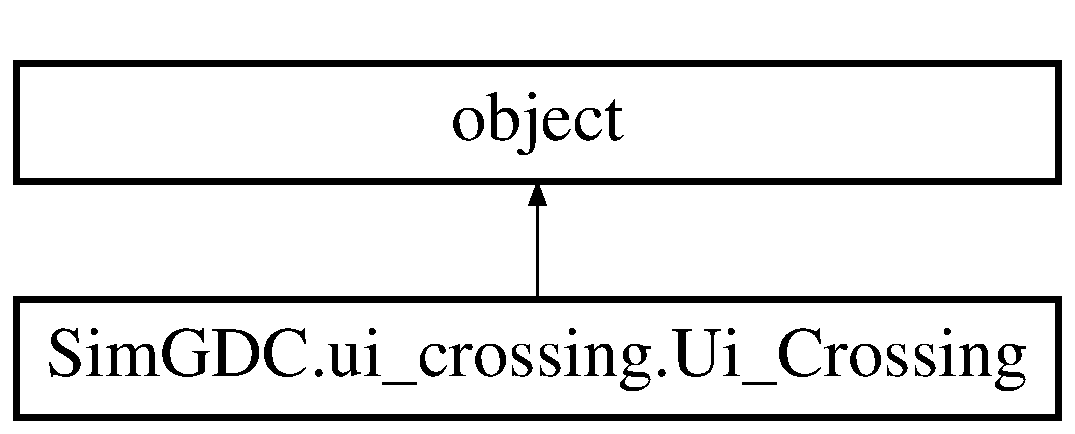
\includegraphics[height=2.000000cm]{class_sim_g_d_c_1_1ui__crossing_1_1_ui___crossing}
\end{center}
\end{figure}
\subsection*{Public Member Functions}
\begin{DoxyCompactItemize}
\item 
\hypertarget{class_sim_g_d_c_1_1ui__crossing_1_1_ui___crossing_afd727a98bc7121d98cd08a546063da6e}{}def {\bfseries setup\+Ui} (self, Crossing)\label{class_sim_g_d_c_1_1ui__crossing_1_1_ui___crossing_afd727a98bc7121d98cd08a546063da6e}

\item 
\hypertarget{class_sim_g_d_c_1_1ui__crossing_1_1_ui___crossing_abe5aad659a739dcfeb3c33af37e51f0b}{}def {\bfseries retranslate\+Ui} (self, Crossing)\label{class_sim_g_d_c_1_1ui__crossing_1_1_ui___crossing_abe5aad659a739dcfeb3c33af37e51f0b}

\end{DoxyCompactItemize}
\subsection*{Public Attributes}
\begin{DoxyCompactItemize}
\item 
\hypertarget{class_sim_g_d_c_1_1ui__crossing_1_1_ui___crossing_a36e3513c82dc9005b1471f18770e9d09}{}{\bfseries grid\+Layout\+\_\+3}\label{class_sim_g_d_c_1_1ui__crossing_1_1_ui___crossing_a36e3513c82dc9005b1471f18770e9d09}

\item 
\hypertarget{class_sim_g_d_c_1_1ui__crossing_1_1_ui___crossing_aee486726cf8eefa44630b88362448635}{}{\bfseries vertical\+Layout}\label{class_sim_g_d_c_1_1ui__crossing_1_1_ui___crossing_aee486726cf8eefa44630b88362448635}

\item 
\hypertarget{class_sim_g_d_c_1_1ui__crossing_1_1_ui___crossing_a04bdce746c5c684ca4c5f9271ca64eb3}{}{\bfseries title\+Label}\label{class_sim_g_d_c_1_1ui__crossing_1_1_ui___crossing_a04bdce746c5c684ca4c5f9271ca64eb3}

\item 
\hypertarget{class_sim_g_d_c_1_1ui__crossing_1_1_ui___crossing_a42719e2ab37629869b939cd0b8b20126}{}{\bfseries Segment\+Group\+Box}\label{class_sim_g_d_c_1_1ui__crossing_1_1_ui___crossing_a42719e2ab37629869b939cd0b8b20126}

\item 
\hypertarget{class_sim_g_d_c_1_1ui__crossing_1_1_ui___crossing_a9bf3d5aec477ec6d89a603685f08eee3}{}{\bfseries grid\+Layout}\label{class_sim_g_d_c_1_1ui__crossing_1_1_ui___crossing_a9bf3d5aec477ec6d89a603685f08eee3}

\item 
\hypertarget{class_sim_g_d_c_1_1ui__crossing_1_1_ui___crossing_aed4c5053af1fcf12e7eca6962f43e2be}{}{\bfseries segment\+Id\+Label}\label{class_sim_g_d_c_1_1ui__crossing_1_1_ui___crossing_aed4c5053af1fcf12e7eca6962f43e2be}

\item 
\hypertarget{class_sim_g_d_c_1_1ui__crossing_1_1_ui___crossing_a3b6b42ba53ec110cf5511ff8f21eff72}{}{\bfseries segment\+Id}\label{class_sim_g_d_c_1_1ui__crossing_1_1_ui___crossing_a3b6b42ba53ec110cf5511ff8f21eff72}

\item 
\hypertarget{class_sim_g_d_c_1_1ui__crossing_1_1_ui___crossing_a4c8f6a323224c1cec25918ecbc1c39cc}{}{\bfseries attribute\+Group}\label{class_sim_g_d_c_1_1ui__crossing_1_1_ui___crossing_a4c8f6a323224c1cec25918ecbc1c39cc}

\item 
\hypertarget{class_sim_g_d_c_1_1ui__crossing_1_1_ui___crossing_a4afe51b7600832e30de3a0c5fcb16d66}{}{\bfseries grid\+Layout\+\_\+2}\label{class_sim_g_d_c_1_1ui__crossing_1_1_ui___crossing_a4afe51b7600832e30de3a0c5fcb16d66}

\item 
\hypertarget{class_sim_g_d_c_1_1ui__crossing_1_1_ui___crossing_a33e30f876da7b4db9f86315c1ccae446}{}{\bfseries horizontal\+Layout}\label{class_sim_g_d_c_1_1ui__crossing_1_1_ui___crossing_a33e30f876da7b4db9f86315c1ccae446}

\item 
\hypertarget{class_sim_g_d_c_1_1ui__crossing_1_1_ui___crossing_afe806565a9d2abcc8656ab242b8bb1ac}{}{\bfseries id\+Label}\label{class_sim_g_d_c_1_1ui__crossing_1_1_ui___crossing_afe806565a9d2abcc8656ab242b8bb1ac}

\item 
\hypertarget{class_sim_g_d_c_1_1ui__crossing_1_1_ui___crossing_ad3752a73329dc4bef61ccd72a214c429}{}{\bfseries id}\label{class_sim_g_d_c_1_1ui__crossing_1_1_ui___crossing_ad3752a73329dc4bef61ccd72a214c429}

\item 
\hypertarget{class_sim_g_d_c_1_1ui__crossing_1_1_ui___crossing_aa7dfc633966f1c3baf07f92913923c17}{}{\bfseries Offset\+Label}\label{class_sim_g_d_c_1_1ui__crossing_1_1_ui___crossing_aa7dfc633966f1c3baf07f92913923c17}

\item 
\hypertarget{class_sim_g_d_c_1_1ui__crossing_1_1_ui___crossing_a5bc0fc82fd6036404cc41b711a64b134}{}{\bfseries offset}\label{class_sim_g_d_c_1_1ui__crossing_1_1_ui___crossing_a5bc0fc82fd6036404cc41b711a64b134}

\item 
\hypertarget{class_sim_g_d_c_1_1ui__crossing_1_1_ui___crossing_a3bb876763ddc0abcd41b6214a90cf5ec}{}{\bfseries splitter}\label{class_sim_g_d_c_1_1ui__crossing_1_1_ui___crossing_a3bb876763ddc0abcd41b6214a90cf5ec}

\item 
\hypertarget{class_sim_g_d_c_1_1ui__crossing_1_1_ui___crossing_ac6c968af5565cbfd7153fd34d6251925}{}{\bfseries error\+Message}\label{class_sim_g_d_c_1_1ui__crossing_1_1_ui___crossing_ac6c968af5565cbfd7153fd34d6251925}

\item 
\hypertarget{class_sim_g_d_c_1_1ui__crossing_1_1_ui___crossing_a314e867845065cd00608d361450153f6}{}{\bfseries action\+Button}\label{class_sim_g_d_c_1_1ui__crossing_1_1_ui___crossing_a314e867845065cd00608d361450153f6}

\end{DoxyCompactItemize}


The documentation for this class was generated from the following file\+:\begin{DoxyCompactItemize}
\item 
ui\+\_\+crossing.\+py\end{DoxyCompactItemize}

\hypertarget{class_sim_g_d_c_1_1ui__lane_1_1_ui___lane}{}\section{Sim\+G\+D\+C.\+ui\+\_\+lane.\+Ui\+\_\+\+Lane Class Reference}
\label{class_sim_g_d_c_1_1ui__lane_1_1_ui___lane}\index{Sim\+G\+D\+C.\+ui\+\_\+lane.\+Ui\+\_\+\+Lane@{Sim\+G\+D\+C.\+ui\+\_\+lane.\+Ui\+\_\+\+Lane}}
Inheritance diagram for Sim\+G\+D\+C.\+ui\+\_\+lane.\+Ui\+\_\+\+Lane\+:\begin{figure}[H]
\begin{center}
\leavevmode
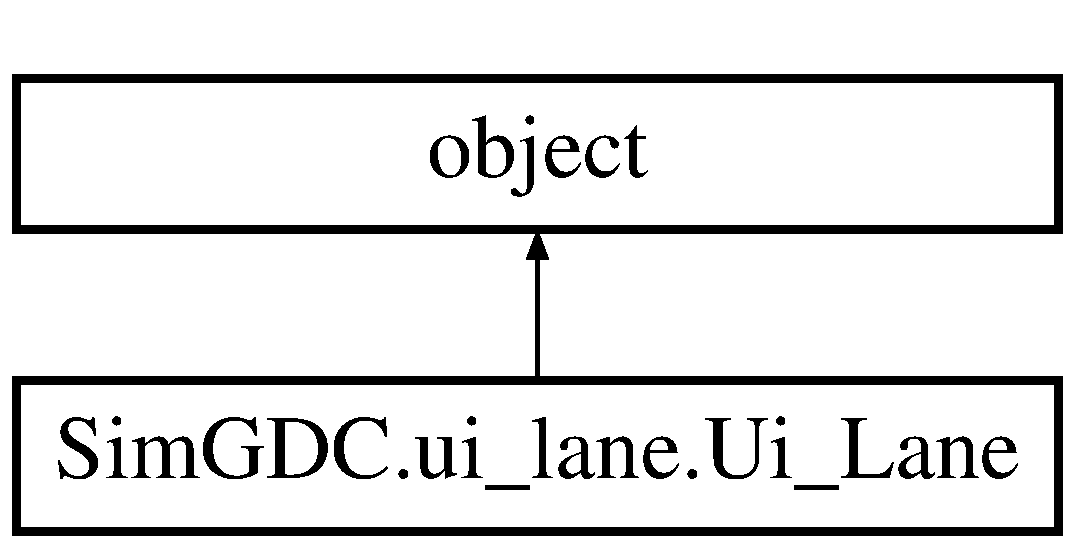
\includegraphics[height=2.000000cm]{class_sim_g_d_c_1_1ui__lane_1_1_ui___lane}
\end{center}
\end{figure}
\subsection*{Public Member Functions}
\begin{DoxyCompactItemize}
\item 
\hypertarget{class_sim_g_d_c_1_1ui__lane_1_1_ui___lane_a0c6fa72d8b6cda3a8bcbb7ac15733217}{}def {\bfseries setup\+Ui} (self, Lane)\label{class_sim_g_d_c_1_1ui__lane_1_1_ui___lane_a0c6fa72d8b6cda3a8bcbb7ac15733217}

\item 
\hypertarget{class_sim_g_d_c_1_1ui__lane_1_1_ui___lane_a137983d33bd1be753722c6c666515fcd}{}def {\bfseries retranslate\+Ui} (self, Lane)\label{class_sim_g_d_c_1_1ui__lane_1_1_ui___lane_a137983d33bd1be753722c6c666515fcd}

\end{DoxyCompactItemize}
\subsection*{Public Attributes}
\begin{DoxyCompactItemize}
\item 
\hypertarget{class_sim_g_d_c_1_1ui__lane_1_1_ui___lane_a3078caf8c05eb3f21724c5d1067ac137}{}{\bfseries tags}\label{class_sim_g_d_c_1_1ui__lane_1_1_ui___lane_a3078caf8c05eb3f21724c5d1067ac137}

\item 
\hypertarget{class_sim_g_d_c_1_1ui__lane_1_1_ui___lane_a90551e844bc3a120c699d2c4c8ce2d72}{}{\bfseries title\+Label}\label{class_sim_g_d_c_1_1ui__lane_1_1_ui___lane_a90551e844bc3a120c699d2c4c8ce2d72}

\item 
\hypertarget{class_sim_g_d_c_1_1ui__lane_1_1_ui___lane_a35f2c2a2de7c21cd50c15892e3e070c1}{}{\bfseries Segment\+Group\+Box}\label{class_sim_g_d_c_1_1ui__lane_1_1_ui___lane_a35f2c2a2de7c21cd50c15892e3e070c1}

\item 
\hypertarget{class_sim_g_d_c_1_1ui__lane_1_1_ui___lane_a6043dfcbe996b1ebe97930dc4f839bce}{}{\bfseries grid\+Layout}\label{class_sim_g_d_c_1_1ui__lane_1_1_ui___lane_a6043dfcbe996b1ebe97930dc4f839bce}

\item 
\hypertarget{class_sim_g_d_c_1_1ui__lane_1_1_ui___lane_afff196ca72147712d985bc2de5552b75}{}{\bfseries segment\+Id\+Label}\label{class_sim_g_d_c_1_1ui__lane_1_1_ui___lane_afff196ca72147712d985bc2de5552b75}

\item 
\hypertarget{class_sim_g_d_c_1_1ui__lane_1_1_ui___lane_a121505539b5eb6e48000cc857de7e9c3}{}{\bfseries segment\+Id}\label{class_sim_g_d_c_1_1ui__lane_1_1_ui___lane_a121505539b5eb6e48000cc857de7e9c3}

\item 
\hypertarget{class_sim_g_d_c_1_1ui__lane_1_1_ui___lane_a42a0906ba8e9c5f8f2efc4f60418d391}{}{\bfseries attribute\+Group}\label{class_sim_g_d_c_1_1ui__lane_1_1_ui___lane_a42a0906ba8e9c5f8f2efc4f60418d391}

\item 
\hypertarget{class_sim_g_d_c_1_1ui__lane_1_1_ui___lane_a00c6cca6e8e15e4ac23a08fb97ff530c}{}{\bfseries vehicle\+Modelabel}\label{class_sim_g_d_c_1_1ui__lane_1_1_ui___lane_a00c6cca6e8e15e4ac23a08fb97ff530c}

\item 
\hypertarget{class_sim_g_d_c_1_1ui__lane_1_1_ui___lane_a9ebb5a9f115ca594662595cf6aa13efc}{}{\bfseries width}\label{class_sim_g_d_c_1_1ui__lane_1_1_ui___lane_a9ebb5a9f115ca594662595cf6aa13efc}

\item 
\hypertarget{class_sim_g_d_c_1_1ui__lane_1_1_ui___lane_a43a0f2b92a908786619b16a1bada9657}{}{\bfseries layout\+Widget}\label{class_sim_g_d_c_1_1ui__lane_1_1_ui___lane_a43a0f2b92a908786619b16a1bada9657}

\item 
\hypertarget{class_sim_g_d_c_1_1ui__lane_1_1_ui___lane_a18e801095a0e276283ac22d6da73e72c}{}{\bfseries horizontal\+Layout}\label{class_sim_g_d_c_1_1ui__lane_1_1_ui___lane_a18e801095a0e276283ac22d6da73e72c}

\item 
\hypertarget{class_sim_g_d_c_1_1ui__lane_1_1_ui___lane_accde822832e89cf576a0ed103df4fc8d}{}{\bfseries can\+\_\+stop}\label{class_sim_g_d_c_1_1ui__lane_1_1_ui___lane_accde822832e89cf576a0ed103df4fc8d}

\item 
\hypertarget{class_sim_g_d_c_1_1ui__lane_1_1_ui___lane_adaffbfa3d31614e1eb26e094e7e4a920}{}{\bfseries high\+\_\+occ\+\_\+veh}\label{class_sim_g_d_c_1_1ui__lane_1_1_ui___lane_adaffbfa3d31614e1eb26e094e7e4a920}

\item 
\hypertarget{class_sim_g_d_c_1_1ui__lane_1_1_ui___lane_a426d5be0db30e89a069112003f342074}{}{\bfseries layout\+Widget1}\label{class_sim_g_d_c_1_1ui__lane_1_1_ui___lane_a426d5be0db30e89a069112003f342074}

\item 
\hypertarget{class_sim_g_d_c_1_1ui__lane_1_1_ui___lane_a6281c2e6771cbc8ad23dbc20ff813d61}{}{\bfseries horizontal\+Layout\+\_\+2}\label{class_sim_g_d_c_1_1ui__lane_1_1_ui___lane_a6281c2e6771cbc8ad23dbc20ff813d61}

\item 
\hypertarget{class_sim_g_d_c_1_1ui__lane_1_1_ui___lane_ad4a4378205f0eb27ddc9b58028c81592}{}{\bfseries can\+\_\+park}\label{class_sim_g_d_c_1_1ui__lane_1_1_ui___lane_ad4a4378205f0eb27ddc9b58028c81592}

\item 
\hypertarget{class_sim_g_d_c_1_1ui__lane_1_1_ui___lane_adeacd711d6e8e7b4b97df4393e7110b4}{}{\bfseries has\+\_\+road\+\_\+shoulder}\label{class_sim_g_d_c_1_1ui__lane_1_1_ui___lane_adeacd711d6e8e7b4b97df4393e7110b4}

\item 
\hypertarget{class_sim_g_d_c_1_1ui__lane_1_1_ui___lane_aef43d20a3c32de6beed3d38f077f0c68}{}{\bfseries layout\+Widget2}\label{class_sim_g_d_c_1_1ui__lane_1_1_ui___lane_aef43d20a3c32de6beed3d38f077f0c68}

\item 
\hypertarget{class_sim_g_d_c_1_1ui__lane_1_1_ui___lane_ae067ca0a661c34816381fa259af2b1c4}{}{\bfseries horizontal\+Layout\+\_\+4}\label{class_sim_g_d_c_1_1ui__lane_1_1_ui___lane_ae067ca0a661c34816381fa259af2b1c4}

\item 
\hypertarget{class_sim_g_d_c_1_1ui__lane_1_1_ui___lane_a2bbd392e786e7e1bb3c153f3824988c3}{}{\bfseries id\+Label}\label{class_sim_g_d_c_1_1ui__lane_1_1_ui___lane_a2bbd392e786e7e1bb3c153f3824988c3}

\item 
\hypertarget{class_sim_g_d_c_1_1ui__lane_1_1_ui___lane_a20299e3c7cf72364174af40b24338209}{}{\bfseries id}\label{class_sim_g_d_c_1_1ui__lane_1_1_ui___lane_a20299e3c7cf72364174af40b24338209}

\item 
\hypertarget{class_sim_g_d_c_1_1ui__lane_1_1_ui___lane_a666d71bfcb612b3bb3a76eebfc0fdcd2}{}{\bfseries width\+Label}\label{class_sim_g_d_c_1_1ui__lane_1_1_ui___lane_a666d71bfcb612b3bb3a76eebfc0fdcd2}

\item 
\hypertarget{class_sim_g_d_c_1_1ui__lane_1_1_ui___lane_a29ed6f6468719eed5141dc0bbb43c96f}{}{\bfseries wline\+Edit}\label{class_sim_g_d_c_1_1ui__lane_1_1_ui___lane_a29ed6f6468719eed5141dc0bbb43c96f}

\item 
\hypertarget{class_sim_g_d_c_1_1ui__lane_1_1_ui___lane_ab20b0d80349c5fc49882bc647073b7bb}{}{\bfseries widget}\label{class_sim_g_d_c_1_1ui__lane_1_1_ui___lane_ab20b0d80349c5fc49882bc647073b7bb}

\item 
\hypertarget{class_sim_g_d_c_1_1ui__lane_1_1_ui___lane_ae0e6b8a8c00dfb82486ffc419b6237fe}{}{\bfseries horizontal\+Layout\+\_\+5}\label{class_sim_g_d_c_1_1ui__lane_1_1_ui___lane_ae0e6b8a8c00dfb82486ffc419b6237fe}

\item 
\hypertarget{class_sim_g_d_c_1_1ui__lane_1_1_ui___lane_a08a038d66737d02d3dacbd06c9ba8d44}{}{\bfseries pedestrian}\label{class_sim_g_d_c_1_1ui__lane_1_1_ui___lane_a08a038d66737d02d3dacbd06c9ba8d44}

\item 
\hypertarget{class_sim_g_d_c_1_1ui__lane_1_1_ui___lane_a67f090bd2bf2ca5665ae388eb4ad7bd6}{}{\bfseries bicycle}\label{class_sim_g_d_c_1_1ui__lane_1_1_ui___lane_a67f090bd2bf2ca5665ae388eb4ad7bd6}

\item 
\hypertarget{class_sim_g_d_c_1_1ui__lane_1_1_ui___lane_a5cea664c991cf35025d1ef7c8d7d7bb0}{}{\bfseries car}\label{class_sim_g_d_c_1_1ui__lane_1_1_ui___lane_a5cea664c991cf35025d1ef7c8d7d7bb0}

\item 
\hypertarget{class_sim_g_d_c_1_1ui__lane_1_1_ui___lane_ae8d2f2b589fa9128f66ee770c2374a44}{}{\bfseries van}\label{class_sim_g_d_c_1_1ui__lane_1_1_ui___lane_ae8d2f2b589fa9128f66ee770c2374a44}

\item 
\hypertarget{class_sim_g_d_c_1_1ui__lane_1_1_ui___lane_a169dfbe4f1aae728618cb961e3eba4d4}{}{\bfseries truck}\label{class_sim_g_d_c_1_1ui__lane_1_1_ui___lane_a169dfbe4f1aae728618cb961e3eba4d4}

\item 
\hypertarget{class_sim_g_d_c_1_1ui__lane_1_1_ui___lane_ab02f4f55a23e60c722942c472aaae66e}{}{\bfseries bus}\label{class_sim_g_d_c_1_1ui__lane_1_1_ui___lane_ab02f4f55a23e60c722942c472aaae66e}

\item 
\hypertarget{class_sim_g_d_c_1_1ui__lane_1_1_ui___lane_aa430fbd0bc536484c87d72b414969663}{}{\bfseries taxi}\label{class_sim_g_d_c_1_1ui__lane_1_1_ui___lane_aa430fbd0bc536484c87d72b414969663}

\item 
\hypertarget{class_sim_g_d_c_1_1ui__lane_1_1_ui___lane_a4bf04ad92f47be64b6971a3993c479a6}{}{\bfseries widget1}\label{class_sim_g_d_c_1_1ui__lane_1_1_ui___lane_a4bf04ad92f47be64b6971a3993c479a6}

\item 
\hypertarget{class_sim_g_d_c_1_1ui__lane_1_1_ui___lane_a8040be6c40d80e042ed275b8633fec8b}{}{\bfseries horizontal\+Layout\+\_\+3}\label{class_sim_g_d_c_1_1ui__lane_1_1_ui___lane_a8040be6c40d80e042ed275b8633fec8b}

\item 
\hypertarget{class_sim_g_d_c_1_1ui__lane_1_1_ui___lane_aaada2c3136e80d18d98d6d66da0c59c9}{}{\bfseries bus\+Lanelabel}\label{class_sim_g_d_c_1_1ui__lane_1_1_ui___lane_aaada2c3136e80d18d98d6d66da0c59c9}

\item 
\hypertarget{class_sim_g_d_c_1_1ui__lane_1_1_ui___lane_aa956779da4c3c4b27bc379e0c7047fca}{}{\bfseries bus\+\_\+lane}\label{class_sim_g_d_c_1_1ui__lane_1_1_ui___lane_aa956779da4c3c4b27bc379e0c7047fca}

\item 
\hypertarget{class_sim_g_d_c_1_1ui__lane_1_1_ui___lane_a9508d7e74dbd07629db3b3dc6e6ea162}{}{\bfseries error\+Message}\label{class_sim_g_d_c_1_1ui__lane_1_1_ui___lane_a9508d7e74dbd07629db3b3dc6e6ea162}

\item 
\hypertarget{class_sim_g_d_c_1_1ui__lane_1_1_ui___lane_aa71d671204e171146f125415f20361b0}{}{\bfseries tagslabel}\label{class_sim_g_d_c_1_1ui__lane_1_1_ui___lane_aa71d671204e171146f125415f20361b0}

\item 
\hypertarget{class_sim_g_d_c_1_1ui__lane_1_1_ui___lane_a222dd6ecafcb2687387e196613adfb12}{}{\bfseries action\+Button}\label{class_sim_g_d_c_1_1ui__lane_1_1_ui___lane_a222dd6ecafcb2687387e196613adfb12}

\end{DoxyCompactItemize}


The documentation for this class was generated from the following file\+:\begin{DoxyCompactItemize}
\item 
ui\+\_\+lane.\+py\end{DoxyCompactItemize}

\hypertarget{class_sim_g_d_c_1_1ui__laneedge_1_1_ui___lane_edge}{}\section{Sim\+G\+D\+C.\+ui\+\_\+laneedge.\+Ui\+\_\+\+Lane\+Edge Class Reference}
\label{class_sim_g_d_c_1_1ui__laneedge_1_1_ui___lane_edge}\index{Sim\+G\+D\+C.\+ui\+\_\+laneedge.\+Ui\+\_\+\+Lane\+Edge@{Sim\+G\+D\+C.\+ui\+\_\+laneedge.\+Ui\+\_\+\+Lane\+Edge}}
Inheritance diagram for Sim\+G\+D\+C.\+ui\+\_\+laneedge.\+Ui\+\_\+\+Lane\+Edge\+:\begin{figure}[H]
\begin{center}
\leavevmode
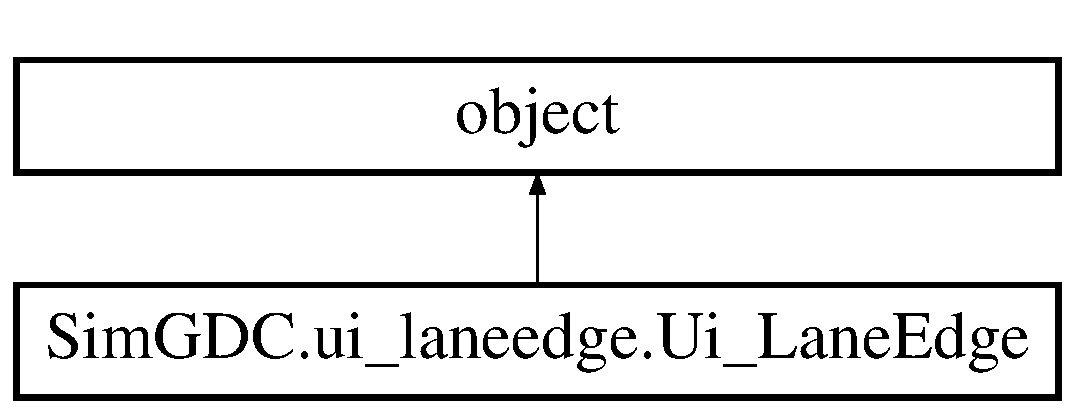
\includegraphics[height=2.000000cm]{class_sim_g_d_c_1_1ui__laneedge_1_1_ui___lane_edge}
\end{center}
\end{figure}
\subsection*{Public Member Functions}
\begin{DoxyCompactItemize}
\item 
\hypertarget{class_sim_g_d_c_1_1ui__laneedge_1_1_ui___lane_edge_ab8f65fdca7aee1e47cfb149b5d5aca0f}{}def {\bfseries setup\+Ui} (self, Lane\+Edge)\label{class_sim_g_d_c_1_1ui__laneedge_1_1_ui___lane_edge_ab8f65fdca7aee1e47cfb149b5d5aca0f}

\item 
\hypertarget{class_sim_g_d_c_1_1ui__laneedge_1_1_ui___lane_edge_a2620fdbe077dcc066de37ab33b82c683}{}def {\bfseries retranslate\+Ui} (self, Lane\+Edge)\label{class_sim_g_d_c_1_1ui__laneedge_1_1_ui___lane_edge_a2620fdbe077dcc066de37ab33b82c683}

\end{DoxyCompactItemize}
\subsection*{Public Attributes}
\begin{DoxyCompactItemize}
\item 
\hypertarget{class_sim_g_d_c_1_1ui__laneedge_1_1_ui___lane_edge_ac0679fa5b87ab669ab80c79a6f7ff30e}{}{\bfseries grid\+Layout\+\_\+3}\label{class_sim_g_d_c_1_1ui__laneedge_1_1_ui___lane_edge_ac0679fa5b87ab669ab80c79a6f7ff30e}

\item 
\hypertarget{class_sim_g_d_c_1_1ui__laneedge_1_1_ui___lane_edge_a61b2fcaa8eabd4328f69eb264ee91feb}{}{\bfseries vertical\+Layout}\label{class_sim_g_d_c_1_1ui__laneedge_1_1_ui___lane_edge_a61b2fcaa8eabd4328f69eb264ee91feb}

\item 
\hypertarget{class_sim_g_d_c_1_1ui__laneedge_1_1_ui___lane_edge_a4ee65e71b1c70a53784e5ed55c986185}{}{\bfseries title\+Label}\label{class_sim_g_d_c_1_1ui__laneedge_1_1_ui___lane_edge_a4ee65e71b1c70a53784e5ed55c986185}

\item 
\hypertarget{class_sim_g_d_c_1_1ui__laneedge_1_1_ui___lane_edge_a245c596fc6d06f2b51d35e5ba0311faa}{}{\bfseries Segment\+Group\+Box}\label{class_sim_g_d_c_1_1ui__laneedge_1_1_ui___lane_edge_a245c596fc6d06f2b51d35e5ba0311faa}

\item 
\hypertarget{class_sim_g_d_c_1_1ui__laneedge_1_1_ui___lane_edge_a992e979ba3836c80d5f00e573f775c8f}{}{\bfseries grid\+Layout}\label{class_sim_g_d_c_1_1ui__laneedge_1_1_ui___lane_edge_a992e979ba3836c80d5f00e573f775c8f}

\item 
\hypertarget{class_sim_g_d_c_1_1ui__laneedge_1_1_ui___lane_edge_a3162ed9580fd6aa5b10db819b367d49b}{}{\bfseries segment\+Id\+Label}\label{class_sim_g_d_c_1_1ui__laneedge_1_1_ui___lane_edge_a3162ed9580fd6aa5b10db819b367d49b}

\item 
\hypertarget{class_sim_g_d_c_1_1ui__laneedge_1_1_ui___lane_edge_a85b5d5fdd3ce1292d214a19c7592b06a}{}{\bfseries segment\+Id}\label{class_sim_g_d_c_1_1ui__laneedge_1_1_ui___lane_edge_a85b5d5fdd3ce1292d214a19c7592b06a}

\item 
\hypertarget{class_sim_g_d_c_1_1ui__laneedge_1_1_ui___lane_edge_ac18b37872966495ba13bc75776f30329}{}{\bfseries attribute\+Group}\label{class_sim_g_d_c_1_1ui__laneedge_1_1_ui___lane_edge_ac18b37872966495ba13bc75776f30329}

\item 
\hypertarget{class_sim_g_d_c_1_1ui__laneedge_1_1_ui___lane_edge_a3523d7450578528abc388a1ece797aed}{}{\bfseries grid\+Layout\+\_\+2}\label{class_sim_g_d_c_1_1ui__laneedge_1_1_ui___lane_edge_a3523d7450578528abc388a1ece797aed}

\item 
\hypertarget{class_sim_g_d_c_1_1ui__laneedge_1_1_ui___lane_edge_a554810270383866df2d905ccc46baf3e}{}{\bfseries lane\+Number\+Label}\label{class_sim_g_d_c_1_1ui__laneedge_1_1_ui___lane_edge_a554810270383866df2d905ccc46baf3e}

\item 
\hypertarget{class_sim_g_d_c_1_1ui__laneedge_1_1_ui___lane_edge_abde32aeafdc6526a42bd5434f8ccc056}{}{\bfseries lane\+Number}\label{class_sim_g_d_c_1_1ui__laneedge_1_1_ui___lane_edge_abde32aeafdc6526a42bd5434f8ccc056}

\item 
\hypertarget{class_sim_g_d_c_1_1ui__laneedge_1_1_ui___lane_edge_a43175d3c3f84e5b05e2079ff99dab072}{}{\bfseries splitter}\label{class_sim_g_d_c_1_1ui__laneedge_1_1_ui___lane_edge_a43175d3c3f84e5b05e2079ff99dab072}

\item 
\hypertarget{class_sim_g_d_c_1_1ui__laneedge_1_1_ui___lane_edge_a89916dd76276d08a4652c952791280d5}{}{\bfseries error\+Message}\label{class_sim_g_d_c_1_1ui__laneedge_1_1_ui___lane_edge_a89916dd76276d08a4652c952791280d5}

\item 
\hypertarget{class_sim_g_d_c_1_1ui__laneedge_1_1_ui___lane_edge_a8ed1b2472b9b5331e29c4f774633e2ed}{}{\bfseries action\+Button}\label{class_sim_g_d_c_1_1ui__laneedge_1_1_ui___lane_edge_a8ed1b2472b9b5331e29c4f774633e2ed}

\end{DoxyCompactItemize}


The documentation for this class was generated from the following file\+:\begin{DoxyCompactItemize}
\item 
ui\+\_\+laneedge.\+py\end{DoxyCompactItemize}

\hypertarget{class_sim_g_d_c_1_1ui__linkmanager_1_1_ui___link_manager}{}\section{Sim\+G\+D\+C.\+ui\+\_\+linkmanager.\+Ui\+\_\+\+Link\+Manager Class Reference}
\label{class_sim_g_d_c_1_1ui__linkmanager_1_1_ui___link_manager}\index{Sim\+G\+D\+C.\+ui\+\_\+linkmanager.\+Ui\+\_\+\+Link\+Manager@{Sim\+G\+D\+C.\+ui\+\_\+linkmanager.\+Ui\+\_\+\+Link\+Manager}}
Inheritance diagram for Sim\+G\+D\+C.\+ui\+\_\+linkmanager.\+Ui\+\_\+\+Link\+Manager\+:\begin{figure}[H]
\begin{center}
\leavevmode
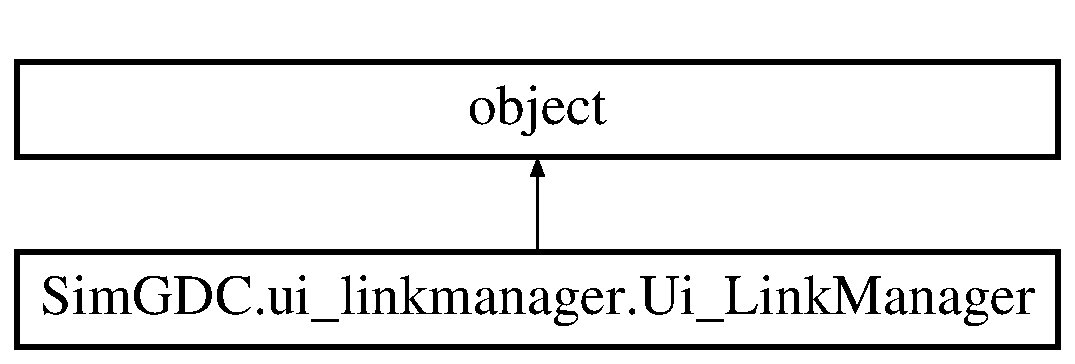
\includegraphics[height=2.000000cm]{class_sim_g_d_c_1_1ui__linkmanager_1_1_ui___link_manager}
\end{center}
\end{figure}
\subsection*{Public Member Functions}
\begin{DoxyCompactItemize}
\item 
\hypertarget{class_sim_g_d_c_1_1ui__linkmanager_1_1_ui___link_manager_ad26aced4b774a9997b524789ba6cbbae}{}def {\bfseries setup\+Ui} (self, Link\+Manager)\label{class_sim_g_d_c_1_1ui__linkmanager_1_1_ui___link_manager_ad26aced4b774a9997b524789ba6cbbae}

\item 
\hypertarget{class_sim_g_d_c_1_1ui__linkmanager_1_1_ui___link_manager_a2d21a8bfbee1060b82f5eabe09c37ed0}{}def {\bfseries retranslate\+Ui} (self, Link\+Manager)\label{class_sim_g_d_c_1_1ui__linkmanager_1_1_ui___link_manager_a2d21a8bfbee1060b82f5eabe09c37ed0}

\end{DoxyCompactItemize}
\subsection*{Public Attributes}
\begin{DoxyCompactItemize}
\item 
\hypertarget{class_sim_g_d_c_1_1ui__linkmanager_1_1_ui___link_manager_a533e513862929428f521045877dfab98}{}{\bfseries attribute\+Group}\label{class_sim_g_d_c_1_1ui__linkmanager_1_1_ui___link_manager_a533e513862929428f521045877dfab98}

\item 
\hypertarget{class_sim_g_d_c_1_1ui__linkmanager_1_1_ui___link_manager_ad5d15d22bcb1f68eb778f0355b2a8f3d}{}{\bfseries action\+Button}\label{class_sim_g_d_c_1_1ui__linkmanager_1_1_ui___link_manager_ad5d15d22bcb1f68eb778f0355b2a8f3d}

\item 
\hypertarget{class_sim_g_d_c_1_1ui__linkmanager_1_1_ui___link_manager_a8aac0f3c7860a7751bf0fa9fca0bfae6}{}{\bfseries categorylabel}\label{class_sim_g_d_c_1_1ui__linkmanager_1_1_ui___link_manager_a8aac0f3c7860a7751bf0fa9fca0bfae6}

\item 
\hypertarget{class_sim_g_d_c_1_1ui__linkmanager_1_1_ui___link_manager_abf17af00c7eb3a62d1154d5fb7f68afa}{}{\bfseries category}\label{class_sim_g_d_c_1_1ui__linkmanager_1_1_ui___link_manager_abf17af00c7eb3a62d1154d5fb7f68afa}

\item 
\hypertarget{class_sim_g_d_c_1_1ui__linkmanager_1_1_ui___link_manager_affbf22537d3c33fd2740dd16512c1783}{}{\bfseries tagslabel}\label{class_sim_g_d_c_1_1ui__linkmanager_1_1_ui___link_manager_affbf22537d3c33fd2740dd16512c1783}

\item 
\hypertarget{class_sim_g_d_c_1_1ui__linkmanager_1_1_ui___link_manager_a4b317d4f1b9a659dca72550d1305e840}{}{\bfseries tags\+Link}\label{class_sim_g_d_c_1_1ui__linkmanager_1_1_ui___link_manager_a4b317d4f1b9a659dca72550d1305e840}

\item 
\hypertarget{class_sim_g_d_c_1_1ui__linkmanager_1_1_ui___link_manager_a6ce9b58ba2fa413a79d54a79dc78646c}{}{\bfseries start\+Node\+Label}\label{class_sim_g_d_c_1_1ui__linkmanager_1_1_ui___link_manager_a6ce9b58ba2fa413a79d54a79dc78646c}

\item 
\hypertarget{class_sim_g_d_c_1_1ui__linkmanager_1_1_ui___link_manager_ab21bfa43313e22ff17bec0234d70daa7}{}{\bfseries end\+Node\+Label}\label{class_sim_g_d_c_1_1ui__linkmanager_1_1_ui___link_manager_ab21bfa43313e22ff17bec0234d70daa7}

\item 
\hypertarget{class_sim_g_d_c_1_1ui__linkmanager_1_1_ui___link_manager_a52b0323510a5d5ff87ffd64eed758506}{}{\bfseries id}\label{class_sim_g_d_c_1_1ui__linkmanager_1_1_ui___link_manager_a52b0323510a5d5ff87ffd64eed758506}

\item 
\hypertarget{class_sim_g_d_c_1_1ui__linkmanager_1_1_ui___link_manager_ae40373d9310a618c06372b4f1fee9a32}{}{\bfseries id\+Label}\label{class_sim_g_d_c_1_1ui__linkmanager_1_1_ui___link_manager_ae40373d9310a618c06372b4f1fee9a32}

\item 
\hypertarget{class_sim_g_d_c_1_1ui__linkmanager_1_1_ui___link_manager_a3a4c82dd13a735fbbb68edf1a5b1f1c3}{}{\bfseries road\+Name\+Label}\label{class_sim_g_d_c_1_1ui__linkmanager_1_1_ui___link_manager_a3a4c82dd13a735fbbb68edf1a5b1f1c3}

\item 
\hypertarget{class_sim_g_d_c_1_1ui__linkmanager_1_1_ui___link_manager_a32b9a2f1d7c9e50622d62d38f5d3899c}{}{\bfseries road\+Name}\label{class_sim_g_d_c_1_1ui__linkmanager_1_1_ui___link_manager_a32b9a2f1d7c9e50622d62d38f5d3899c}

\item 
\hypertarget{class_sim_g_d_c_1_1ui__linkmanager_1_1_ui___link_manager_aaf22749cea19408f5136185ebf4d55dd}{}{\bfseries road\+Type\+Label}\label{class_sim_g_d_c_1_1ui__linkmanager_1_1_ui___link_manager_aaf22749cea19408f5136185ebf4d55dd}

\item 
\hypertarget{class_sim_g_d_c_1_1ui__linkmanager_1_1_ui___link_manager_a81a644ef04db6087cd51f510576f0bb1}{}{\bfseries road\+Type}\label{class_sim_g_d_c_1_1ui__linkmanager_1_1_ui___link_manager_a81a644ef04db6087cd51f510576f0bb1}

\item 
\hypertarget{class_sim_g_d_c_1_1ui__linkmanager_1_1_ui___link_manager_a9912ce243682685a68aa43995de4ecd8}{}{\bfseries start\+Node}\label{class_sim_g_d_c_1_1ui__linkmanager_1_1_ui___link_manager_a9912ce243682685a68aa43995de4ecd8}

\item 
\hypertarget{class_sim_g_d_c_1_1ui__linkmanager_1_1_ui___link_manager_ac286cc6e5812e125a5ce4285810c4845}{}{\bfseries end\+Node}\label{class_sim_g_d_c_1_1ui__linkmanager_1_1_ui___link_manager_ac286cc6e5812e125a5ce4285810c4845}

\item 
\hypertarget{class_sim_g_d_c_1_1ui__linkmanager_1_1_ui___link_manager_a5b0e02f192d201398dd8de40e7f6238e}{}{\bfseries title\+Label}\label{class_sim_g_d_c_1_1ui__linkmanager_1_1_ui___link_manager_a5b0e02f192d201398dd8de40e7f6238e}

\item 
\hypertarget{class_sim_g_d_c_1_1ui__linkmanager_1_1_ui___link_manager_a7431b76749612b5f52261cc78baa362f}{}{\bfseries link\+Group\+Box}\label{class_sim_g_d_c_1_1ui__linkmanager_1_1_ui___link_manager_a7431b76749612b5f52261cc78baa362f}

\item 
\hypertarget{class_sim_g_d_c_1_1ui__linkmanager_1_1_ui___link_manager_a7cc7ce9ceef240be107d88c60f7ce120}{}{\bfseries link\+Id\+Label}\label{class_sim_g_d_c_1_1ui__linkmanager_1_1_ui___link_manager_a7cc7ce9ceef240be107d88c60f7ce120}

\item 
\hypertarget{class_sim_g_d_c_1_1ui__linkmanager_1_1_ui___link_manager_aec0ba87d5f626dc177ff26a7c33f505f}{}{\bfseries link\+Id\+Combo\+Box}\label{class_sim_g_d_c_1_1ui__linkmanager_1_1_ui___link_manager_aec0ba87d5f626dc177ff26a7c33f505f}

\item 
\hypertarget{class_sim_g_d_c_1_1ui__linkmanager_1_1_ui___link_manager_a56c1a64d013ba9c5890889ff8c7b00bb}{}{\bfseries error\+Message}\label{class_sim_g_d_c_1_1ui__linkmanager_1_1_ui___link_manager_a56c1a64d013ba9c5890889ff8c7b00bb}

\end{DoxyCompactItemize}


The documentation for this class was generated from the following file\+:\begin{DoxyCompactItemize}
\item 
ui\+\_\+linkmanager.\+py\end{DoxyCompactItemize}

\hypertarget{class_sim_g_d_c_1_1ui__multinode_1_1_ui___multi_node}{}\section{Sim\+G\+D\+C.\+ui\+\_\+multinode.\+Ui\+\_\+\+Multi\+Node Class Reference}
\label{class_sim_g_d_c_1_1ui__multinode_1_1_ui___multi_node}\index{Sim\+G\+D\+C.\+ui\+\_\+multinode.\+Ui\+\_\+\+Multi\+Node@{Sim\+G\+D\+C.\+ui\+\_\+multinode.\+Ui\+\_\+\+Multi\+Node}}
Inheritance diagram for Sim\+G\+D\+C.\+ui\+\_\+multinode.\+Ui\+\_\+\+Multi\+Node\+:\begin{figure}[H]
\begin{center}
\leavevmode
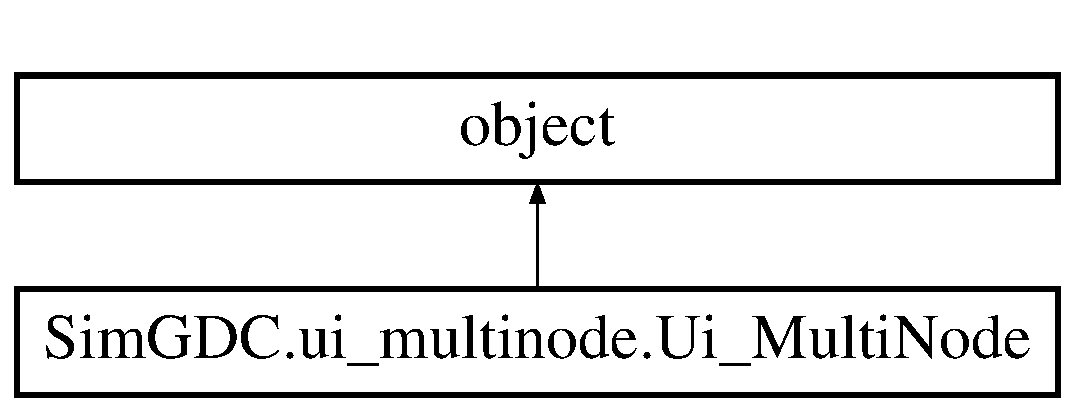
\includegraphics[height=2.000000cm]{class_sim_g_d_c_1_1ui__multinode_1_1_ui___multi_node}
\end{center}
\end{figure}
\subsection*{Public Member Functions}
\begin{DoxyCompactItemize}
\item 
\hypertarget{class_sim_g_d_c_1_1ui__multinode_1_1_ui___multi_node_a346c704a6a16c2cba223cb11d0345d3b}{}def {\bfseries setup\+Ui} (self, Multi\+Node)\label{class_sim_g_d_c_1_1ui__multinode_1_1_ui___multi_node_a346c704a6a16c2cba223cb11d0345d3b}

\item 
\hypertarget{class_sim_g_d_c_1_1ui__multinode_1_1_ui___multi_node_a043bd7569f92e5d6c025db1411aabfa4}{}def {\bfseries retranslate\+Ui} (self, Multi\+Node)\label{class_sim_g_d_c_1_1ui__multinode_1_1_ui___multi_node_a043bd7569f92e5d6c025db1411aabfa4}

\end{DoxyCompactItemize}
\subsection*{Public Attributes}
\begin{DoxyCompactItemize}
\item 
\hypertarget{class_sim_g_d_c_1_1ui__multinode_1_1_ui___multi_node_afd4b998091ecc82efac8964ae7f01f59}{}{\bfseries grid\+Layout\+\_\+4}\label{class_sim_g_d_c_1_1ui__multinode_1_1_ui___multi_node_afd4b998091ecc82efac8964ae7f01f59}

\item 
\hypertarget{class_sim_g_d_c_1_1ui__multinode_1_1_ui___multi_node_a30191100f360ae1edf4f007b3ac148f5}{}{\bfseries tab\+Widget}\label{class_sim_g_d_c_1_1ui__multinode_1_1_ui___multi_node_a30191100f360ae1edf4f007b3ac148f5}

\item 
\hypertarget{class_sim_g_d_c_1_1ui__multinode_1_1_ui___multi_node_a475059790daeb0badefbd1ce2cfd4342}{}{\bfseries tab}\label{class_sim_g_d_c_1_1ui__multinode_1_1_ui___multi_node_a475059790daeb0badefbd1ce2cfd4342}

\item 
\hypertarget{class_sim_g_d_c_1_1ui__multinode_1_1_ui___multi_node_a781f44dff663870f1c07b9fce0c4b9ba}{}{\bfseries Traffic\+Light\+I\+Dlabel}\label{class_sim_g_d_c_1_1ui__multinode_1_1_ui___multi_node_a781f44dff663870f1c07b9fce0c4b9ba}

\item 
\hypertarget{class_sim_g_d_c_1_1ui__multinode_1_1_ui___multi_node_a209feb5e045739188253cb8a68eec3d8}{}{\bfseries Node\+Typelabel}\label{class_sim_g_d_c_1_1ui__multinode_1_1_ui___multi_node_a209feb5e045739188253cb8a68eec3d8}

\item 
\hypertarget{class_sim_g_d_c_1_1ui__multinode_1_1_ui___multi_node_ad266481f8e6cbf905f4c46932ad5962d}{}{\bfseries node\+Type}\label{class_sim_g_d_c_1_1ui__multinode_1_1_ui___multi_node_ad266481f8e6cbf905f4c46932ad5962d}

\item 
\hypertarget{class_sim_g_d_c_1_1ui__multinode_1_1_ui___multi_node_ac7a3a83767b411475d71a1a42988546e}{}{\bfseries traffic\+Light\+I\+D}\label{class_sim_g_d_c_1_1ui__multinode_1_1_ui___multi_node_ac7a3a83767b411475d71a1a42988546e}

\item 
\hypertarget{class_sim_g_d_c_1_1ui__multinode_1_1_ui___multi_node_a54a2e50fb350545a65152418594d2eee}{}{\bfseries attribute\+Group}\label{class_sim_g_d_c_1_1ui__multinode_1_1_ui___multi_node_a54a2e50fb350545a65152418594d2eee}

\item 
\hypertarget{class_sim_g_d_c_1_1ui__multinode_1_1_ui___multi_node_a33c551c97526dc6520ffb774be63aef4}{}{\bfseries grid\+Layout}\label{class_sim_g_d_c_1_1ui__multinode_1_1_ui___multi_node_a33c551c97526dc6520ffb774be63aef4}

\item 
\hypertarget{class_sim_g_d_c_1_1ui__multinode_1_1_ui___multi_node_a32d1886783a14d47a143aeb77982bc5d}{}{\bfseries horizontal\+Layout}\label{class_sim_g_d_c_1_1ui__multinode_1_1_ui___multi_node_a32d1886783a14d47a143aeb77982bc5d}

\item 
\hypertarget{class_sim_g_d_c_1_1ui__multinode_1_1_ui___multi_node_a163a440e1abe64a5bafd6e488db9368d}{}{\bfseries node\+Id\+Label}\label{class_sim_g_d_c_1_1ui__multinode_1_1_ui___multi_node_a163a440e1abe64a5bafd6e488db9368d}

\item 
\hypertarget{class_sim_g_d_c_1_1ui__multinode_1_1_ui___multi_node_a449412f195713338daf96e529d1364c6}{}{\bfseries node\+Id}\label{class_sim_g_d_c_1_1ui__multinode_1_1_ui___multi_node_a449412f195713338daf96e529d1364c6}

\item 
\hypertarget{class_sim_g_d_c_1_1ui__multinode_1_1_ui___multi_node_af629c90558c7668fc2ed596f61782cb1}{}{\bfseries splitter}\label{class_sim_g_d_c_1_1ui__multinode_1_1_ui___multi_node_af629c90558c7668fc2ed596f61782cb1}

\item 
\hypertarget{class_sim_g_d_c_1_1ui__multinode_1_1_ui___multi_node_ad7a31a4915dccfa13253fab34d65abf0}{}{\bfseries error\+Message}\label{class_sim_g_d_c_1_1ui__multinode_1_1_ui___multi_node_ad7a31a4915dccfa13253fab34d65abf0}

\item 
\hypertarget{class_sim_g_d_c_1_1ui__multinode_1_1_ui___multi_node_acc1e8585487a6b989826b55673d2bc5c}{}{\bfseries action\+Button}\label{class_sim_g_d_c_1_1ui__multinode_1_1_ui___multi_node_acc1e8585487a6b989826b55673d2bc5c}

\item 
\hypertarget{class_sim_g_d_c_1_1ui__multinode_1_1_ui___multi_node_a09f25d1ca9e3b879f16b604bb82b2923}{}{\bfseries tags\+\_\+node\+\_\+label}\label{class_sim_g_d_c_1_1ui__multinode_1_1_ui___multi_node_a09f25d1ca9e3b879f16b604bb82b2923}

\item 
\hypertarget{class_sim_g_d_c_1_1ui__multinode_1_1_ui___multi_node_a4fa443a8fc2dcaf7d27528b66beff4f5}{}{\bfseries tags\+\_\+node}\label{class_sim_g_d_c_1_1ui__multinode_1_1_ui___multi_node_a4fa443a8fc2dcaf7d27528b66beff4f5}

\item 
\hypertarget{class_sim_g_d_c_1_1ui__multinode_1_1_ui___multi_node_afd6b1cf55801885bae46bcba09996dc9}{}{\bfseries tab\+\_\+3}\label{class_sim_g_d_c_1_1ui__multinode_1_1_ui___multi_node_afd6b1cf55801885bae46bcba09996dc9}

\item 
\hypertarget{class_sim_g_d_c_1_1ui__multinode_1_1_ui___multi_node_a78e7ff9ef6428c238f1fba76d776e632}{}{\bfseries turning\+Group}\label{class_sim_g_d_c_1_1ui__multinode_1_1_ui___multi_node_a78e7ff9ef6428c238f1fba76d776e632}

\item 
\hypertarget{class_sim_g_d_c_1_1ui__multinode_1_1_ui___multi_node_a5f4e429fa666a2b53a5639afc2598cc8}{}{\bfseries turning\+Group\+I\+Dlabel}\label{class_sim_g_d_c_1_1ui__multinode_1_1_ui___multi_node_a5f4e429fa666a2b53a5639afc2598cc8}

\item 
\hypertarget{class_sim_g_d_c_1_1ui__multinode_1_1_ui___multi_node_a513c0c06e634cd9a6c0c83d787b26e9f}{}{\bfseries turning\+Group\+I\+D}\label{class_sim_g_d_c_1_1ui__multinode_1_1_ui___multi_node_a513c0c06e634cd9a6c0c83d787b26e9f}

\item 
\hypertarget{class_sim_g_d_c_1_1ui__multinode_1_1_ui___multi_node_a77375aacd18becf25347007779218676}{}{\bfseries from\+Linklabel}\label{class_sim_g_d_c_1_1ui__multinode_1_1_ui___multi_node_a77375aacd18becf25347007779218676}

\item 
\hypertarget{class_sim_g_d_c_1_1ui__multinode_1_1_ui___multi_node_a2176557f20e0c94138ca5feeb02bdf43}{}{\bfseries from\+Link}\label{class_sim_g_d_c_1_1ui__multinode_1_1_ui___multi_node_a2176557f20e0c94138ca5feeb02bdf43}

\item 
\hypertarget{class_sim_g_d_c_1_1ui__multinode_1_1_ui___multi_node_aa042ea466319087d79bc91bc15365a87}{}{\bfseries to\+Linklabel}\label{class_sim_g_d_c_1_1ui__multinode_1_1_ui___multi_node_aa042ea466319087d79bc91bc15365a87}

\item 
\hypertarget{class_sim_g_d_c_1_1ui__multinode_1_1_ui___multi_node_af17e2aed08f1b712a36362fe244b0f88}{}{\bfseries to\+Link}\label{class_sim_g_d_c_1_1ui__multinode_1_1_ui___multi_node_af17e2aed08f1b712a36362fe244b0f88}

\item 
\hypertarget{class_sim_g_d_c_1_1ui__multinode_1_1_ui___multi_node_a4c33a25d31f317469a0e6b07934f6c2c}{}{\bfseries Phaseslabel}\label{class_sim_g_d_c_1_1ui__multinode_1_1_ui___multi_node_a4c33a25d31f317469a0e6b07934f6c2c}

\item 
\hypertarget{class_sim_g_d_c_1_1ui__multinode_1_1_ui___multi_node_a8837c2cdd83eae2552dac4341e776e89}{}{\bfseries Rules}\label{class_sim_g_d_c_1_1ui__multinode_1_1_ui___multi_node_a8837c2cdd83eae2552dac4341e776e89}

\item 
\hypertarget{class_sim_g_d_c_1_1ui__multinode_1_1_ui___multi_node_ac10d6f00f2570ffe63932218b233a69a}{}{\bfseries Ruleslabel}\label{class_sim_g_d_c_1_1ui__multinode_1_1_ui___multi_node_ac10d6f00f2570ffe63932218b233a69a}

\item 
\hypertarget{class_sim_g_d_c_1_1ui__multinode_1_1_ui___multi_node_acd98f74c6f09907522cd7cc360943bb4}{}{\bfseries newturning\+Group}\label{class_sim_g_d_c_1_1ui__multinode_1_1_ui___multi_node_acd98f74c6f09907522cd7cc360943bb4}

\item 
\hypertarget{class_sim_g_d_c_1_1ui__multinode_1_1_ui___multi_node_ac4d8a529732e5f0ef391027e0ea445b3}{}{\bfseries Phases}\label{class_sim_g_d_c_1_1ui__multinode_1_1_ui___multi_node_ac4d8a529732e5f0ef391027e0ea445b3}

\item 
\hypertarget{class_sim_g_d_c_1_1ui__multinode_1_1_ui___multi_node_a62f3440f54e565231ec4f3a7a0d30686}{}{\bfseries visibility\+\_\+distance\+\_\+label}\label{class_sim_g_d_c_1_1ui__multinode_1_1_ui___multi_node_a62f3440f54e565231ec4f3a7a0d30686}

\item 
\hypertarget{class_sim_g_d_c_1_1ui__multinode_1_1_ui___multi_node_a7ce06700d2dc44d1496cf9ffa0e44413}{}{\bfseries visibility\+\_\+distance}\label{class_sim_g_d_c_1_1ui__multinode_1_1_ui___multi_node_a7ce06700d2dc44d1496cf9ffa0e44413}

\item 
\hypertarget{class_sim_g_d_c_1_1ui__multinode_1_1_ui___multi_node_a1c49810c1f57b40682ffe66bebd6408c}{}{\bfseries tags\+\_\+turninggroup}\label{class_sim_g_d_c_1_1ui__multinode_1_1_ui___multi_node_a1c49810c1f57b40682ffe66bebd6408c}

\item 
\hypertarget{class_sim_g_d_c_1_1ui__multinode_1_1_ui___multi_node_ab53f97c4a1be41758f79b70b7ddfeb62}{}{\bfseries tags\+\_\+tg\+\_\+label}\label{class_sim_g_d_c_1_1ui__multinode_1_1_ui___multi_node_ab53f97c4a1be41758f79b70b7ddfeb62}

\item 
\hypertarget{class_sim_g_d_c_1_1ui__multinode_1_1_ui___multi_node_a331114c298f7ecb1d95ce796ce5cb023}{}{\bfseries delturninggroup\+Button}\label{class_sim_g_d_c_1_1ui__multinode_1_1_ui___multi_node_a331114c298f7ecb1d95ce796ce5cb023}

\item 
\hypertarget{class_sim_g_d_c_1_1ui__multinode_1_1_ui___multi_node_a2f60d5234ec45b185a83ad89643da5d4}{}{\bfseries Turning\+Group\+Table}\label{class_sim_g_d_c_1_1ui__multinode_1_1_ui___multi_node_a2f60d5234ec45b185a83ad89643da5d4}

\item 
\hypertarget{class_sim_g_d_c_1_1ui__multinode_1_1_ui___multi_node_ab3dfd25b3484da44f231b5d6a8b324ea}{}{\bfseries turning\+Path}\label{class_sim_g_d_c_1_1ui__multinode_1_1_ui___multi_node_ab3dfd25b3484da44f231b5d6a8b324ea}

\item 
\hypertarget{class_sim_g_d_c_1_1ui__multinode_1_1_ui___multi_node_a244e053f5d0576492d21b4fa34844b2f}{}{\bfseries Turning\+Path\+I\+Dlabel}\label{class_sim_g_d_c_1_1ui__multinode_1_1_ui___multi_node_a244e053f5d0576492d21b4fa34844b2f}

\item 
\hypertarget{class_sim_g_d_c_1_1ui__multinode_1_1_ui___multi_node_a3ef461558370e02bf1455b4509922d17}{}{\bfseries Turning\+Path}\label{class_sim_g_d_c_1_1ui__multinode_1_1_ui___multi_node_a3ef461558370e02bf1455b4509922d17}

\item 
\hypertarget{class_sim_g_d_c_1_1ui__multinode_1_1_ui___multi_node_af5b18d8b7cedf125ab5764a7a258d5ed}{}{\bfseries from\+Lanelabel}\label{class_sim_g_d_c_1_1ui__multinode_1_1_ui___multi_node_af5b18d8b7cedf125ab5764a7a258d5ed}

\item 
\hypertarget{class_sim_g_d_c_1_1ui__multinode_1_1_ui___multi_node_af36bef6da45c57cb028113a3b4952c28}{}{\bfseries from\+Lane}\label{class_sim_g_d_c_1_1ui__multinode_1_1_ui___multi_node_af36bef6da45c57cb028113a3b4952c28}

\item 
\hypertarget{class_sim_g_d_c_1_1ui__multinode_1_1_ui___multi_node_a5c2a975fe60e2d1dc32c6755fa6363a0}{}{\bfseries to\+Lanelabel}\label{class_sim_g_d_c_1_1ui__multinode_1_1_ui___multi_node_a5c2a975fe60e2d1dc32c6755fa6363a0}

\item 
\hypertarget{class_sim_g_d_c_1_1ui__multinode_1_1_ui___multi_node_a6198ebda674321ee4264458467364390}{}{\bfseries to\+Lane}\label{class_sim_g_d_c_1_1ui__multinode_1_1_ui___multi_node_a6198ebda674321ee4264458467364390}

\item 
\hypertarget{class_sim_g_d_c_1_1ui__multinode_1_1_ui___multi_node_ae26b2c851600862a1a29e9311d0e98ac}{}{\bfseries new\+Turning\+Path}\label{class_sim_g_d_c_1_1ui__multinode_1_1_ui___multi_node_ae26b2c851600862a1a29e9311d0e98ac}

\item 
\hypertarget{class_sim_g_d_c_1_1ui__multinode_1_1_ui___multi_node_a846224a578369f377c62b30573e400e6}{}{\bfseries max\+Speed\+\_\+label}\label{class_sim_g_d_c_1_1ui__multinode_1_1_ui___multi_node_a846224a578369f377c62b30573e400e6}

\item 
\hypertarget{class_sim_g_d_c_1_1ui__multinode_1_1_ui___multi_node_afd095a589dac3d09e7a9cd0e7f3eed47}{}{\bfseries tags\+\_\+turningpath}\label{class_sim_g_d_c_1_1ui__multinode_1_1_ui___multi_node_afd095a589dac3d09e7a9cd0e7f3eed47}

\item 
\hypertarget{class_sim_g_d_c_1_1ui__multinode_1_1_ui___multi_node_a3b91ce20fbacbe119a208f5d817f9761}{}{\bfseries tagts\+\_\+tp\+\_\+label}\label{class_sim_g_d_c_1_1ui__multinode_1_1_ui___multi_node_a3b91ce20fbacbe119a208f5d817f9761}

\item 
\hypertarget{class_sim_g_d_c_1_1ui__multinode_1_1_ui___multi_node_aac8a7d8bc776b81981fb1c2fb878d87e}{}{\bfseries delturningpath\+Button}\label{class_sim_g_d_c_1_1ui__multinode_1_1_ui___multi_node_aac8a7d8bc776b81981fb1c2fb878d87e}

\item 
\hypertarget{class_sim_g_d_c_1_1ui__multinode_1_1_ui___multi_node_ae93fdb8c00ca50ce905a104ecd280c98}{}{\bfseries Turning\+Path\+Table}\label{class_sim_g_d_c_1_1ui__multinode_1_1_ui___multi_node_ae93fdb8c00ca50ce905a104ecd280c98}

\item 
\hypertarget{class_sim_g_d_c_1_1ui__multinode_1_1_ui___multi_node_a40737b5a4c7f8f06c8195c67163cf2dc}{}{\bfseries max\+Speed}\label{class_sim_g_d_c_1_1ui__multinode_1_1_ui___multi_node_a40737b5a4c7f8f06c8195c67163cf2dc}

\item 
\hypertarget{class_sim_g_d_c_1_1ui__multinode_1_1_ui___multi_node_a9f2b033c39196a09c361d8f942e96d08}{}{\bfseries tab\+\_\+2}\label{class_sim_g_d_c_1_1ui__multinode_1_1_ui___multi_node_a9f2b033c39196a09c361d8f942e96d08}

\item 
\hypertarget{class_sim_g_d_c_1_1ui__multinode_1_1_ui___multi_node_abffeb1ba0841a4c0d17610746ea990ed}{}{\bfseries Turning\+Conflict\+Table}\label{class_sim_g_d_c_1_1ui__multinode_1_1_ui___multi_node_abffeb1ba0841a4c0d17610746ea990ed}

\item 
\hypertarget{class_sim_g_d_c_1_1ui__multinode_1_1_ui___multi_node_a5e892ecd1f70bf3d6ff251dec95d7a1d}{}{\bfseries genconflictbutton}\label{class_sim_g_d_c_1_1ui__multinode_1_1_ui___multi_node_a5e892ecd1f70bf3d6ff251dec95d7a1d}

\end{DoxyCompactItemize}


The documentation for this class was generated from the following file\+:\begin{DoxyCompactItemize}
\item 
ui\+\_\+multinode.\+py\end{DoxyCompactItemize}

\hypertarget{class_sim_g_d_c_1_1ui__segment_1_1_ui___segment}{}\section{Sim\+G\+D\+C.\+ui\+\_\+segment.\+Ui\+\_\+\+Segment Class Reference}
\label{class_sim_g_d_c_1_1ui__segment_1_1_ui___segment}\index{Sim\+G\+D\+C.\+ui\+\_\+segment.\+Ui\+\_\+\+Segment@{Sim\+G\+D\+C.\+ui\+\_\+segment.\+Ui\+\_\+\+Segment}}
Inheritance diagram for Sim\+G\+D\+C.\+ui\+\_\+segment.\+Ui\+\_\+\+Segment\+:\begin{figure}[H]
\begin{center}
\leavevmode
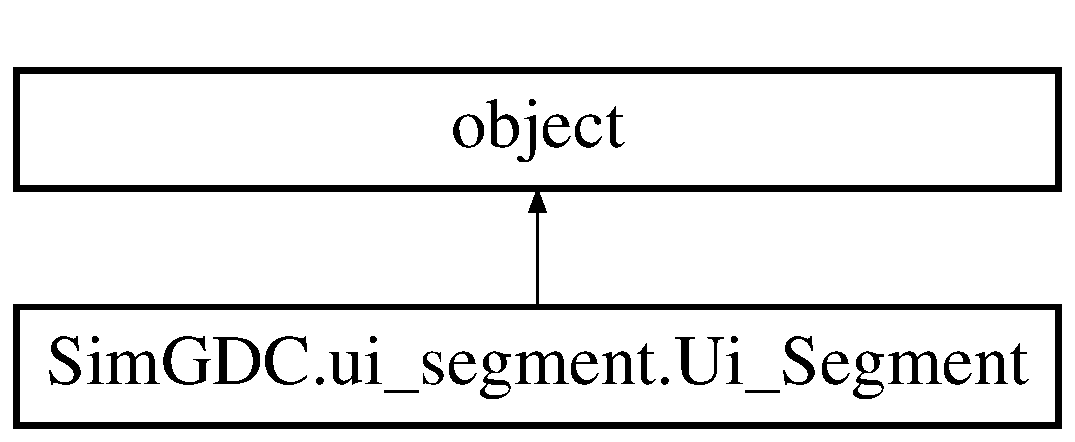
\includegraphics[height=2.000000cm]{class_sim_g_d_c_1_1ui__segment_1_1_ui___segment}
\end{center}
\end{figure}
\subsection*{Public Member Functions}
\begin{DoxyCompactItemize}
\item 
\hypertarget{class_sim_g_d_c_1_1ui__segment_1_1_ui___segment_a10cefb620f1d10aff0a68cc57fffb7b4}{}def {\bfseries setup\+Ui} (self, Segment)\label{class_sim_g_d_c_1_1ui__segment_1_1_ui___segment_a10cefb620f1d10aff0a68cc57fffb7b4}

\item 
\hypertarget{class_sim_g_d_c_1_1ui__segment_1_1_ui___segment_aec890a7a37e5ffaf4dd92931afa2e871}{}def {\bfseries retranslate\+Ui} (self, Segment)\label{class_sim_g_d_c_1_1ui__segment_1_1_ui___segment_aec890a7a37e5ffaf4dd92931afa2e871}

\end{DoxyCompactItemize}
\subsection*{Public Attributes}
\begin{DoxyCompactItemize}
\item 
\hypertarget{class_sim_g_d_c_1_1ui__segment_1_1_ui___segment_a266dfdd6a82d1797ab3987cc36c1c620}{}{\bfseries tab\+Widget\+\_\+2}\label{class_sim_g_d_c_1_1ui__segment_1_1_ui___segment_a266dfdd6a82d1797ab3987cc36c1c620}

\item 
\hypertarget{class_sim_g_d_c_1_1ui__segment_1_1_ui___segment_a847aca14a9c8d1807fa0c2b1e09fa50a}{}{\bfseries tab\+\_\+2}\label{class_sim_g_d_c_1_1ui__segment_1_1_ui___segment_a847aca14a9c8d1807fa0c2b1e09fa50a}

\item 
\hypertarget{class_sim_g_d_c_1_1ui__segment_1_1_ui___segment_a85e1e5719eae449660907c53aaca6567}{}{\bfseries title\+Label}\label{class_sim_g_d_c_1_1ui__segment_1_1_ui___segment_a85e1e5719eae449660907c53aaca6567}

\item 
\hypertarget{class_sim_g_d_c_1_1ui__segment_1_1_ui___segment_a5cdc9cce8ce460000d92656ad2bdb462}{}{\bfseries error\+Message\+\_\+2}\label{class_sim_g_d_c_1_1ui__segment_1_1_ui___segment_a5cdc9cce8ce460000d92656ad2bdb462}

\item 
\hypertarget{class_sim_g_d_c_1_1ui__segment_1_1_ui___segment_a3330ac0fa9582bebd2ba65858ebb8f52}{}{\bfseries link\+Group\+Box}\label{class_sim_g_d_c_1_1ui__segment_1_1_ui___segment_a3330ac0fa9582bebd2ba65858ebb8f52}

\item 
\hypertarget{class_sim_g_d_c_1_1ui__segment_1_1_ui___segment_ad05be8412ecb0b0a504d428a880d8163}{}{\bfseries link\+Id\+Label}\label{class_sim_g_d_c_1_1ui__segment_1_1_ui___segment_ad05be8412ecb0b0a504d428a880d8163}

\item 
\hypertarget{class_sim_g_d_c_1_1ui__segment_1_1_ui___segment_aa74ef1aa2e5be67e8864514cba86033d}{}{\bfseries linkidcombo\+Box}\label{class_sim_g_d_c_1_1ui__segment_1_1_ui___segment_aa74ef1aa2e5be67e8864514cba86033d}

\item 
\hypertarget{class_sim_g_d_c_1_1ui__segment_1_1_ui___segment_a22c293540afd8518ea2e22a5a457960c}{}{\bfseries attribute\+Group\+\_\+2}\label{class_sim_g_d_c_1_1ui__segment_1_1_ui___segment_a22c293540afd8518ea2e22a5a457960c}

\item 
\hypertarget{class_sim_g_d_c_1_1ui__segment_1_1_ui___segment_abacaaf44270ad39782468af0972de792}{}{\bfseries link\+Id\+Combo\+Box}\label{class_sim_g_d_c_1_1ui__segment_1_1_ui___segment_abacaaf44270ad39782468af0972de792}

\item 
\hypertarget{class_sim_g_d_c_1_1ui__segment_1_1_ui___segment_aa260e9b367fe2f5ffee7eb9fa3147427}{}{\bfseries Tags}\label{class_sim_g_d_c_1_1ui__segment_1_1_ui___segment_aa260e9b367fe2f5ffee7eb9fa3147427}

\item 
\hypertarget{class_sim_g_d_c_1_1ui__segment_1_1_ui___segment_adddf250b7d15b8fca13e59939dddbee3}{}{\bfseries taglabel}\label{class_sim_g_d_c_1_1ui__segment_1_1_ui___segment_adddf250b7d15b8fca13e59939dddbee3}

\item 
\hypertarget{class_sim_g_d_c_1_1ui__segment_1_1_ui___segment_a8d5d50848ce8b33b40bcfecbafd5c8e8}{}{\bfseries action\+Button}\label{class_sim_g_d_c_1_1ui__segment_1_1_ui___segment_a8d5d50848ce8b33b40bcfecbafd5c8e8}

\item 
\hypertarget{class_sim_g_d_c_1_1ui__segment_1_1_ui___segment_a5448e25f2a79d10bf7aec08f674778e2}{}{\bfseries layout\+Widget}\label{class_sim_g_d_c_1_1ui__segment_1_1_ui___segment_a5448e25f2a79d10bf7aec08f674778e2}

\item 
\hypertarget{class_sim_g_d_c_1_1ui__segment_1_1_ui___segment_a5423c2c1ec56024025e47f687d0d8a74}{}{\bfseries horizontal\+Layout}\label{class_sim_g_d_c_1_1ui__segment_1_1_ui___segment_a5423c2c1ec56024025e47f687d0d8a74}

\item 
\hypertarget{class_sim_g_d_c_1_1ui__segment_1_1_ui___segment_adb17db0aaef90bb9124b1fbc20b48792}{}{\bfseries id\+Label}\label{class_sim_g_d_c_1_1ui__segment_1_1_ui___segment_adb17db0aaef90bb9124b1fbc20b48792}

\item 
\hypertarget{class_sim_g_d_c_1_1ui__segment_1_1_ui___segment_a18188d653e14b86ffdf30c79d1ecaa92}{}{\bfseries id}\label{class_sim_g_d_c_1_1ui__segment_1_1_ui___segment_a18188d653e14b86ffdf30c79d1ecaa92}

\item 
\hypertarget{class_sim_g_d_c_1_1ui__segment_1_1_ui___segment_a156441d88d2586bd613edeec0fbf259c}{}{\bfseries max\+Speed\+Label}\label{class_sim_g_d_c_1_1ui__segment_1_1_ui___segment_a156441d88d2586bd613edeec0fbf259c}

\item 
\hypertarget{class_sim_g_d_c_1_1ui__segment_1_1_ui___segment_abd5e16186881af2ee356f1cbbd27ae92}{}{\bfseries max\+Speed}\label{class_sim_g_d_c_1_1ui__segment_1_1_ui___segment_abd5e16186881af2ee356f1cbbd27ae92}

\item 
\hypertarget{class_sim_g_d_c_1_1ui__segment_1_1_ui___segment_a31deac504d05b0f203e6b4e05e6ea7a0}{}{\bfseries layout\+Widget1}\label{class_sim_g_d_c_1_1ui__segment_1_1_ui___segment_a31deac504d05b0f203e6b4e05e6ea7a0}

\item 
\hypertarget{class_sim_g_d_c_1_1ui__segment_1_1_ui___segment_afb61497c2013c0ecadd502d71c377eb9}{}{\bfseries horizontal\+Layout\+\_\+2}\label{class_sim_g_d_c_1_1ui__segment_1_1_ui___segment_afb61497c2013c0ecadd502d71c377eb9}

\item 
\hypertarget{class_sim_g_d_c_1_1ui__segment_1_1_ui___segment_aec7e20a28a7862d6f162d2720168b2e1}{}{\bfseries sequenceno\+Label}\label{class_sim_g_d_c_1_1ui__segment_1_1_ui___segment_aec7e20a28a7862d6f162d2720168b2e1}

\item 
\hypertarget{class_sim_g_d_c_1_1ui__segment_1_1_ui___segment_afc12cb9bbffd6da77582fd4692819674}{}{\bfseries sequenceno}\label{class_sim_g_d_c_1_1ui__segment_1_1_ui___segment_afc12cb9bbffd6da77582fd4692819674}

\item 
\hypertarget{class_sim_g_d_c_1_1ui__segment_1_1_ui___segment_a4ed4f50ecdca7e8a21d166d056777898}{}{\bfseries capacity\+Label}\label{class_sim_g_d_c_1_1ui__segment_1_1_ui___segment_a4ed4f50ecdca7e8a21d166d056777898}

\item 
\hypertarget{class_sim_g_d_c_1_1ui__segment_1_1_ui___segment_a9f4c177e36908b7a16d882326951e644}{}{\bfseries capacity}\label{class_sim_g_d_c_1_1ui__segment_1_1_ui___segment_a9f4c177e36908b7a16d882326951e644}

\item 
\hypertarget{class_sim_g_d_c_1_1ui__segment_1_1_ui___segment_a0327a45f681a90fdaa5427d088da4469}{}{\bfseries tab\+\_\+4}\label{class_sim_g_d_c_1_1ui__segment_1_1_ui___segment_a0327a45f681a90fdaa5427d088da4469}

\item 
\hypertarget{class_sim_g_d_c_1_1ui__segment_1_1_ui___segment_a6c7ac3a7cad882730f5b70ffcabdf2a6}{}{\bfseries label}\label{class_sim_g_d_c_1_1ui__segment_1_1_ui___segment_a6c7ac3a7cad882730f5b70ffcabdf2a6}

\item 
\hypertarget{class_sim_g_d_c_1_1ui__segment_1_1_ui___segment_af680f3ca3e26f24be03f2b06c522e5d3}{}{\bfseries lane\+I\+D}\label{class_sim_g_d_c_1_1ui__segment_1_1_ui___segment_af680f3ca3e26f24be03f2b06c522e5d3}

\item 
\hypertarget{class_sim_g_d_c_1_1ui__segment_1_1_ui___segment_af913e4aa9228d16c77cd339cfb0dc31c}{}{\bfseries laneidlabel}\label{class_sim_g_d_c_1_1ui__segment_1_1_ui___segment_af913e4aa9228d16c77cd339cfb0dc31c}

\item 
\hypertarget{class_sim_g_d_c_1_1ui__segment_1_1_ui___segment_a6c37d4cdb3d7abad849fd30e2922d067}{}{\bfseries from\+Sectionlabel}\label{class_sim_g_d_c_1_1ui__segment_1_1_ui___segment_a6c37d4cdb3d7abad849fd30e2922d067}

\item 
\hypertarget{class_sim_g_d_c_1_1ui__segment_1_1_ui___segment_ad903fe3a5b4c67a1479b270a46f197f0}{}{\bfseries from\+Sectioncombo\+Box}\label{class_sim_g_d_c_1_1ui__segment_1_1_ui___segment_ad903fe3a5b4c67a1479b270a46f197f0}

\item 
\hypertarget{class_sim_g_d_c_1_1ui__segment_1_1_ui___segment_ae4e7b1d50a0a11391790c473f8e6f214}{}{\bfseries to\+Sectionlabel}\label{class_sim_g_d_c_1_1ui__segment_1_1_ui___segment_ae4e7b1d50a0a11391790c473f8e6f214}

\item 
\hypertarget{class_sim_g_d_c_1_1ui__segment_1_1_ui___segment_abf26a7ab2e7737fcd28c8f7cf19a7056}{}{\bfseries to\+Sectioncombo\+Box}\label{class_sim_g_d_c_1_1ui__segment_1_1_ui___segment_abf26a7ab2e7737fcd28c8f7cf19a7056}

\item 
\hypertarget{class_sim_g_d_c_1_1ui__segment_1_1_ui___segment_a1f5caee55d9b4360f298be491d14ded5}{}{\bfseries from\+Lanelabel}\label{class_sim_g_d_c_1_1ui__segment_1_1_ui___segment_a1f5caee55d9b4360f298be491d14ded5}

\item 
\hypertarget{class_sim_g_d_c_1_1ui__segment_1_1_ui___segment_a2d7d6ba8eb4b458a979a2a0c8afdf300}{}{\bfseries to\+Lanelabel}\label{class_sim_g_d_c_1_1ui__segment_1_1_ui___segment_a2d7d6ba8eb4b458a979a2a0c8afdf300}

\item 
\hypertarget{class_sim_g_d_c_1_1ui__segment_1_1_ui___segment_a025ccdfcf461f98493d373007f8fc5b4}{}{\bfseries to\+Lanecombo\+Box}\label{class_sim_g_d_c_1_1ui__segment_1_1_ui___segment_a025ccdfcf461f98493d373007f8fc5b4}

\item 
\hypertarget{class_sim_g_d_c_1_1ui__segment_1_1_ui___segment_a30e4b39e3c4f894ebe6cea0365365911}{}{\bfseries from\+Lanecombo\+Box}\label{class_sim_g_d_c_1_1ui__segment_1_1_ui___segment_a30e4b39e3c4f894ebe6cea0365365911}

\item 
\hypertarget{class_sim_g_d_c_1_1ui__segment_1_1_ui___segment_a8ba8e1128c9e98f2fcbdaf7ae7a3aa10}{}{\bfseries lane\+Connector\+Table}\label{class_sim_g_d_c_1_1ui__segment_1_1_ui___segment_a8ba8e1128c9e98f2fcbdaf7ae7a3aa10}

\item 
\hypertarget{class_sim_g_d_c_1_1ui__segment_1_1_ui___segment_a112e02977aa48e42e37048ca079ca45e}{}{\bfseries push\+Button}\label{class_sim_g_d_c_1_1ui__segment_1_1_ui___segment_a112e02977aa48e42e37048ca079ca45e}

\item 
\hypertarget{class_sim_g_d_c_1_1ui__segment_1_1_ui___segment_acffb4bcabe5bb5cecb280f0576f33b2f}{}{\bfseries del\+Button}\label{class_sim_g_d_c_1_1ui__segment_1_1_ui___segment_acffb4bcabe5bb5cecb280f0576f33b2f}

\end{DoxyCompactItemize}


The documentation for this class was generated from the following file\+:\begin{DoxyCompactItemize}
\item 
ui\+\_\+segment.\+py\end{DoxyCompactItemize}

\hypertarget{class_sim_g_d_c_1_1ui__trainstop_1_1_ui___train_stop}{}\section{Sim\+G\+D\+C.\+ui\+\_\+trainstop.\+Ui\+\_\+\+Train\+Stop Class Reference}
\label{class_sim_g_d_c_1_1ui__trainstop_1_1_ui___train_stop}\index{Sim\+G\+D\+C.\+ui\+\_\+trainstop.\+Ui\+\_\+\+Train\+Stop@{Sim\+G\+D\+C.\+ui\+\_\+trainstop.\+Ui\+\_\+\+Train\+Stop}}
Inheritance diagram for Sim\+G\+D\+C.\+ui\+\_\+trainstop.\+Ui\+\_\+\+Train\+Stop\+:\begin{figure}[H]
\begin{center}
\leavevmode
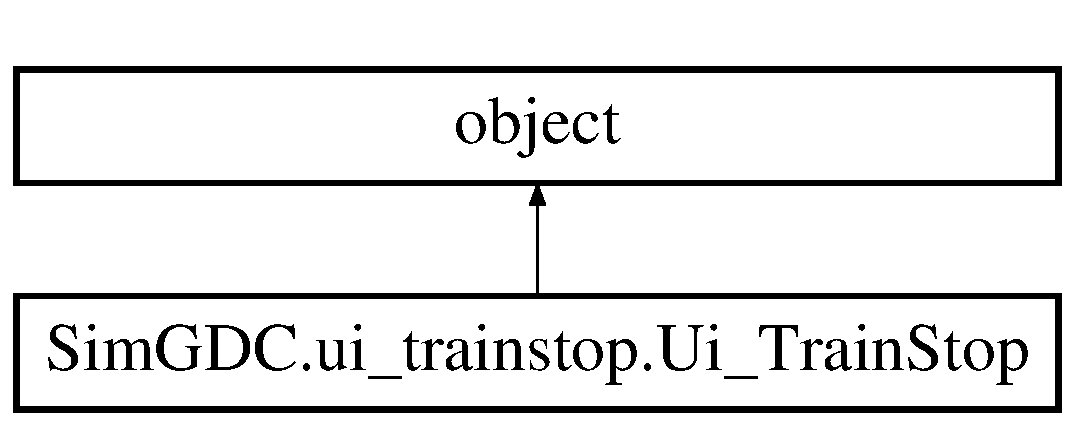
\includegraphics[height=2.000000cm]{class_sim_g_d_c_1_1ui__trainstop_1_1_ui___train_stop}
\end{center}
\end{figure}
\subsection*{Public Member Functions}
\begin{DoxyCompactItemize}
\item 
\hypertarget{class_sim_g_d_c_1_1ui__trainstop_1_1_ui___train_stop_a655a957585643809fa986721970c62d6}{}def {\bfseries setup\+Ui} (self, Train\+Stop)\label{class_sim_g_d_c_1_1ui__trainstop_1_1_ui___train_stop_a655a957585643809fa986721970c62d6}

\item 
\hypertarget{class_sim_g_d_c_1_1ui__trainstop_1_1_ui___train_stop_a71cfc605841a3aebc7ef39869fe2edd9}{}def {\bfseries retranslate\+Ui} (self, Train\+Stop)\label{class_sim_g_d_c_1_1ui__trainstop_1_1_ui___train_stop_a71cfc605841a3aebc7ef39869fe2edd9}

\end{DoxyCompactItemize}
\subsection*{Public Attributes}
\begin{DoxyCompactItemize}
\item 
\hypertarget{class_sim_g_d_c_1_1ui__trainstop_1_1_ui___train_stop_a448d44a85ba8c7955a23b4f3825d8062}{}{\bfseries push\+Button}\label{class_sim_g_d_c_1_1ui__trainstop_1_1_ui___train_stop_a448d44a85ba8c7955a23b4f3825d8062}

\item 
\hypertarget{class_sim_g_d_c_1_1ui__trainstop_1_1_ui___train_stop_a713cb3ae04d07eaca7575d518a89c320}{}{\bfseries Segment\+Group\+Box}\label{class_sim_g_d_c_1_1ui__trainstop_1_1_ui___train_stop_a713cb3ae04d07eaca7575d518a89c320}

\item 
\hypertarget{class_sim_g_d_c_1_1ui__trainstop_1_1_ui___train_stop_ac00d7e6a1c69e78265b096367aa2ff03}{}{\bfseries segment\+I\+Dlabel}\label{class_sim_g_d_c_1_1ui__trainstop_1_1_ui___train_stop_ac00d7e6a1c69e78265b096367aa2ff03}

\item 
\hypertarget{class_sim_g_d_c_1_1ui__trainstop_1_1_ui___train_stop_a1740ed3e2e3851cfdaa30a46ea550731}{}{\bfseries segment\+I\+Dcombo\+Box}\label{class_sim_g_d_c_1_1ui__trainstop_1_1_ui___train_stop_a1740ed3e2e3851cfdaa30a46ea550731}

\item 
\hypertarget{class_sim_g_d_c_1_1ui__trainstop_1_1_ui___train_stop_acf0ca82018a6583df9ab1bc75a871b40}{}{\bfseries label}\label{class_sim_g_d_c_1_1ui__trainstop_1_1_ui___train_stop_acf0ca82018a6583df9ab1bc75a871b40}

\item 
\hypertarget{class_sim_g_d_c_1_1ui__trainstop_1_1_ui___train_stop_a4d4c056817b017b53370eac0e7edf5a4}{}{\bfseries segments\+List\+Line\+Edit}\label{class_sim_g_d_c_1_1ui__trainstop_1_1_ui___train_stop_a4d4c056817b017b53370eac0e7edf5a4}

\item 
\hypertarget{class_sim_g_d_c_1_1ui__trainstop_1_1_ui___train_stop_a6c6ad5eaeface5df5450dd11b09aaad1}{}{\bfseries id\+Label}\label{class_sim_g_d_c_1_1ui__trainstop_1_1_ui___train_stop_a6c6ad5eaeface5df5450dd11b09aaad1}

\item 
\hypertarget{class_sim_g_d_c_1_1ui__trainstop_1_1_ui___train_stop_a6d4054882974f9f1767bf7250b9c6b72}{}{\bfseries id}\label{class_sim_g_d_c_1_1ui__trainstop_1_1_ui___train_stop_a6d4054882974f9f1767bf7250b9c6b72}

\item 
\hypertarget{class_sim_g_d_c_1_1ui__trainstop_1_1_ui___train_stop_a94ee9874b9c61dd25952e35385ed21eb}{}{\bfseries platform\+Namelabel}\label{class_sim_g_d_c_1_1ui__trainstop_1_1_ui___train_stop_a94ee9874b9c61dd25952e35385ed21eb}

\item 
\hypertarget{class_sim_g_d_c_1_1ui__trainstop_1_1_ui___train_stop_a00d99dc5b18ade6a07476b336dd49283}{}{\bfseries station\+Namelabel}\label{class_sim_g_d_c_1_1ui__trainstop_1_1_ui___train_stop_a00d99dc5b18ade6a07476b336dd49283}

\item 
\hypertarget{class_sim_g_d_c_1_1ui__trainstop_1_1_ui___train_stop_ae1c64e4bb2e86ccec6a4b947697ba591}{}{\bfseries type\+Label}\label{class_sim_g_d_c_1_1ui__trainstop_1_1_ui___train_stop_ae1c64e4bb2e86ccec6a4b947697ba591}

\item 
\hypertarget{class_sim_g_d_c_1_1ui__trainstop_1_1_ui___train_stop_aa1984fb9ec93bb7af1f1eda7d670f058}{}{\bfseries tags\+Label}\label{class_sim_g_d_c_1_1ui__trainstop_1_1_ui___train_stop_aa1984fb9ec93bb7af1f1eda7d670f058}

\item 
\hypertarget{class_sim_g_d_c_1_1ui__trainstop_1_1_ui___train_stop_a4ecc8e4db9a592125654c907564b3477}{}{\bfseries platform\+\_\+name}\label{class_sim_g_d_c_1_1ui__trainstop_1_1_ui___train_stop_a4ecc8e4db9a592125654c907564b3477}

\item 
\hypertarget{class_sim_g_d_c_1_1ui__trainstop_1_1_ui___train_stop_a4461c270fd74c31796787e8ff90d9b1e}{}{\bfseries station\+\_\+name}\label{class_sim_g_d_c_1_1ui__trainstop_1_1_ui___train_stop_a4461c270fd74c31796787e8ff90d9b1e}

\item 
\hypertarget{class_sim_g_d_c_1_1ui__trainstop_1_1_ui___train_stop_a75cc6c24c050cf7d4f084890c5524207}{}{\bfseries tags}\label{class_sim_g_d_c_1_1ui__trainstop_1_1_ui___train_stop_a75cc6c24c050cf7d4f084890c5524207}

\item 
\hypertarget{class_sim_g_d_c_1_1ui__trainstop_1_1_ui___train_stop_aec2abdf0672fba06bf8d337c00aa3b78}{}{\bfseries type}\label{class_sim_g_d_c_1_1ui__trainstop_1_1_ui___train_stop_aec2abdf0672fba06bf8d337c00aa3b78}

\item 
\hypertarget{class_sim_g_d_c_1_1ui__trainstop_1_1_ui___train_stop_aac5af35f77d84bd14ced09a9dcc44327}{}{\bfseries Train\+Stoplabel}\label{class_sim_g_d_c_1_1ui__trainstop_1_1_ui___train_stop_aac5af35f77d84bd14ced09a9dcc44327}

\end{DoxyCompactItemize}


The documentation for this class was generated from the following file\+:\begin{DoxyCompactItemize}
\item 
ui\+\_\+trainstop.\+py\end{DoxyCompactItemize}

\hypertarget{class_sim_g_d_c_1_1xml_to_shapefile_1_1_xml_to_shapefile}{}\section{Sim\+G\+D\+C.\+xml\+To\+Shapefile.\+Xml\+To\+Shapefile Class Reference}
\label{class_sim_g_d_c_1_1xml_to_shapefile_1_1_xml_to_shapefile}\index{Sim\+G\+D\+C.\+xml\+To\+Shapefile.\+Xml\+To\+Shapefile@{Sim\+G\+D\+C.\+xml\+To\+Shapefile.\+Xml\+To\+Shapefile}}
Inheritance diagram for Sim\+G\+D\+C.\+xml\+To\+Shapefile.\+Xml\+To\+Shapefile\+:\begin{figure}[H]
\begin{center}
\leavevmode
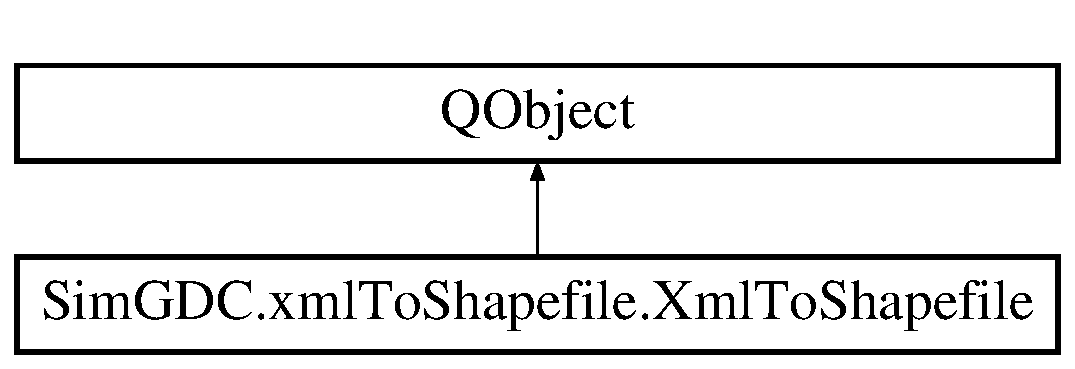
\includegraphics[height=2.000000cm]{class_sim_g_d_c_1_1xml_to_shapefile_1_1_xml_to_shapefile}
\end{center}
\end{figure}
\subsection*{Public Member Functions}
\begin{DoxyCompactItemize}
\item 
\hypertarget{class_sim_g_d_c_1_1xml_to_shapefile_1_1_xml_to_shapefile_a54876d2977cbce6b4f1b0c57295fa454}{}def {\bfseries \+\_\+\+\_\+init\+\_\+\+\_\+} (self, xml\+\_\+path, sh\+\_\+dir, formula)\label{class_sim_g_d_c_1_1xml_to_shapefile_1_1_xml_to_shapefile_a54876d2977cbce6b4f1b0c57295fa454}

\item 
\hypertarget{class_sim_g_d_c_1_1xml_to_shapefile_1_1_xml_to_shapefile_a49083777f1e59d198bc799e7c855fa9f}{}def {\bfseries parse\+Location} (self, data)\label{class_sim_g_d_c_1_1xml_to_shapefile_1_1_xml_to_shapefile_a49083777f1e59d198bc799e7c855fa9f}

\item 
\hypertarget{class_sim_g_d_c_1_1xml_to_shapefile_1_1_xml_to_shapefile_afddf2f688037ba1351a98847da9b21aa}{}def {\bfseries parse\+Mulnode} (self, mulnode)\label{class_sim_g_d_c_1_1xml_to_shapefile_1_1_xml_to_shapefile_afddf2f688037ba1351a98847da9b21aa}

\item 
\hypertarget{class_sim_g_d_c_1_1xml_to_shapefile_1_1_xml_to_shapefile_aca03be00a423101ca396b35900149beb}{}def {\bfseries parse\+Lane} (self, segment\+Id, lane)\label{class_sim_g_d_c_1_1xml_to_shapefile_1_1_xml_to_shapefile_aca03be00a423101ca396b35900149beb}

\item 
\hypertarget{class_sim_g_d_c_1_1xml_to_shapefile_1_1_xml_to_shapefile_af4fd769b80d72f503c478e50ce2cca80}{}def {\bfseries parse\+Lane\+Edge} (self, segment\+Id, lane\+Edge)\label{class_sim_g_d_c_1_1xml_to_shapefile_1_1_xml_to_shapefile_af4fd769b80d72f503c478e50ce2cca80}

\item 
\hypertarget{class_sim_g_d_c_1_1xml_to_shapefile_1_1_xml_to_shapefile_a29dafa7d6f33140b8fa21d73c0146e73}{}def {\bfseries parse\+Crossing} (self, segment\+Id, crossing)\label{class_sim_g_d_c_1_1xml_to_shapefile_1_1_xml_to_shapefile_a29dafa7d6f33140b8fa21d73c0146e73}

\item 
\hypertarget{class_sim_g_d_c_1_1xml_to_shapefile_1_1_xml_to_shapefile_a679eaac2d99684b4eac2420f99bb4293}{}def {\bfseries parse\+Turning\+Path} (self, turningpath)\label{class_sim_g_d_c_1_1xml_to_shapefile_1_1_xml_to_shapefile_a679eaac2d99684b4eac2420f99bb4293}

\item 
\hypertarget{class_sim_g_d_c_1_1xml_to_shapefile_1_1_xml_to_shapefile_aade9c10875762b5f301e3a7031e49df4}{}def {\bfseries parse\+Link} (self, link)\label{class_sim_g_d_c_1_1xml_to_shapefile_1_1_xml_to_shapefile_aade9c10875762b5f301e3a7031e49df4}

\item 
\hypertarget{class_sim_g_d_c_1_1xml_to_shapefile_1_1_xml_to_shapefile_aa0bd3ef84532177e8d51e99bc3d2930d}{}def {\bfseries parse\+Busstop} (self, busstop)\label{class_sim_g_d_c_1_1xml_to_shapefile_1_1_xml_to_shapefile_aa0bd3ef84532177e8d51e99bc3d2930d}

\item 
\hypertarget{class_sim_g_d_c_1_1xml_to_shapefile_1_1_xml_to_shapefile_ae15ad29b692075c20430dd65fb860f3f}{}def {\bfseries parse\+Trainstop} (self, trainstop)\label{class_sim_g_d_c_1_1xml_to_shapefile_1_1_xml_to_shapefile_ae15ad29b692075c20430dd65fb860f3f}

\item 
\hypertarget{class_sim_g_d_c_1_1xml_to_shapefile_1_1_xml_to_shapefile_a86ab25326c08ef3268d98b7174769163}{}def {\bfseries parse\+Segment} (self, link\+Id, segment)\label{class_sim_g_d_c_1_1xml_to_shapefile_1_1_xml_to_shapefile_a86ab25326c08ef3268d98b7174769163}

\item 
\hypertarget{class_sim_g_d_c_1_1xml_to_shapefile_1_1_xml_to_shapefile_a92e9694ae4d0b6524c5fab56e276ae0c}{}def {\bfseries run} (self)\label{class_sim_g_d_c_1_1xml_to_shapefile_1_1_xml_to_shapefile_a92e9694ae4d0b6524c5fab56e276ae0c}

\end{DoxyCompactItemize}
\subsection*{Public Attributes}
\begin{DoxyCompactItemize}
\item 
\hypertarget{class_sim_g_d_c_1_1xml_to_shapefile_1_1_xml_to_shapefile_ab611e1477e7b9b69b83f9f516548812f}{}{\bfseries document}\label{class_sim_g_d_c_1_1xml_to_shapefile_1_1_xml_to_shapefile_ab611e1477e7b9b69b83f9f516548812f}

\item 
\hypertarget{class_sim_g_d_c_1_1xml_to_shapefile_1_1_xml_to_shapefile_a6a1525ba603ca4f873b8b1715cb0635c}{}{\bfseries writer}\label{class_sim_g_d_c_1_1xml_to_shapefile_1_1_xml_to_shapefile_a6a1525ba603ca4f873b8b1715cb0635c}

\item 
\hypertarget{class_sim_g_d_c_1_1xml_to_shapefile_1_1_xml_to_shapefile_a62dd7ff19bc3bc85e070f54701798a5a}{}{\bfseries formula}\label{class_sim_g_d_c_1_1xml_to_shapefile_1_1_xml_to_shapefile_a62dd7ff19bc3bc85e070f54701798a5a}

\end{DoxyCompactItemize}
\subsection*{Static Public Attributes}
\begin{DoxyCompactItemize}
\item 
\hypertarget{class_sim_g_d_c_1_1xml_to_shapefile_1_1_xml_to_shapefile_a4a1ee8f5c6f2294550f905aa88dbab3d}{}tuple {\bfseries prog\+\_\+sig} = pyqt\+Signal(int)\label{class_sim_g_d_c_1_1xml_to_shapefile_1_1_xml_to_shapefile_a4a1ee8f5c6f2294550f905aa88dbab3d}

\end{DoxyCompactItemize}


The documentation for this class was generated from the following file\+:\begin{DoxyCompactItemize}
\item 
xml\+To\+Shapefile.\+py\end{DoxyCompactItemize}

%--- End generated contents ---

% Index
\backmatter
\newpage
\phantomsection
\clearemptydoublepage
\addcontentsline{toc}{chapter}{Index}
\printindex

\end{document}
